\documentclass[12pt,a4paper,oneside]{report}
\renewcommand{\baselinestretch}{1.5}
%---------------spacing between number and caption in lof-------------------- 
\makeatletter
     \renewcommand*\l@figure{\@dottedtocline{1}{1em}{3em}}
\makeatother
%------------Required Packages------------------------------------------------
\usepackage[english]{babel}
\addto{\captionsenglish}{\renewcommand{\bibname}{References}}
%-------------Multirow and multocolomn table-----------------------------------
\usepackage{multirow}
%---------------COLOR----------------------------------------------------------
\usepackage[dvipsnames]{xcolor}
\definecolor{ured}{HTML}{C00000}
\definecolor{ublue}{HTML}{0000FF}
%-----------------section numbering--------------------------------------------
\setcounter{tocdepth}{3}
\setcounter{secnumdepth}{3}
%------------------------------------------------------------------------------
\usepackage{cite}
%\usepackage{tcolorbox}
%------------------Math font and symbols---------------------------------------
\usepackage{amsmath}
\usepackage{amsfonts}
\usepackage{amssymb}
%-----------------------Theroum definition lemma--------------------------------
\usepackage{amsthm}
\theoremstyle{definition}
\newtheorem{definition}{Definition}[section]
\newtheorem{corollary}{Corollary}
%-------------------------Add figures-------------------------------------------
\usepackage{graphicx}
\graphicspath{ {images/} }
%-------------------------table------------------------------------------------
\usepackage{booktabs}
\usepackage{threeparttable}
\usepackage{float}
%------------------------------------------------------------------------------
\usepackage{array}
\usepackage[hidelinks]{hyperref}
\hypersetup{linktoc=all,}

\usepackage[left=1.5in,right=1in,top=1in,bottom=1in]{geometry}

%-----------------------Nomenclature Setting------------------------------------
\usepackage{nomencl}
\nomlabelwidth=3cm 
\makenomenclature
\renewcommand{\nomname}{Abbreviations}
%--------------------------Contents Name----------------------------------------
\addto\captionsenglish{\renewcommand{\contentsname}{INTENT}}
%---------------------for removing hyperindentation-----------------------------
\brokenpenalty=10000
\hyphenpenalty=10000
%-----------------------numbered discription------------------------------------
\usepackage{enumitem}
\newcounter{descriptcount}
\renewcommand*\thedescriptcount{\arabic{descriptcount}}
%------------------------figure numbering---------------------------------------
\usepackage{chngcntr}
\counterwithin{figure}{section}
\counterwithin{table}{section}
%\renewcommand{\thefigure}{\arabic{chapter}.\arabic{section}.\arabic{figure}}
%\renewcommand{\thetable}{\arabic{chapter}.\arabic{section}.\arabic{table}}
%-------------------------Indent to zero-------------------------------------
\setlength{\parindent}{0pt}
%------------------------landscape package-------------------------------------
\usepackage{pdflscape}
%\begin{landscape}
%\end{landscape
%---------------------------rotate figure--------------------------------------
\usepackage{rotating}
%\begin{sidewaysfigure}
%\end{sidewaysfigure}

%\begin{figure} 
%   \centering 
%   \begin{turn}{90}
%   \includegraphics[scale=0.60]{333.png}
%   \end{turn}
%   \caption{ MSCI Sector performances.} 
%   \label{Fig:16} 
%\end{figure}

%\begin{sidewaysfigure}} 
%   \centering 
%   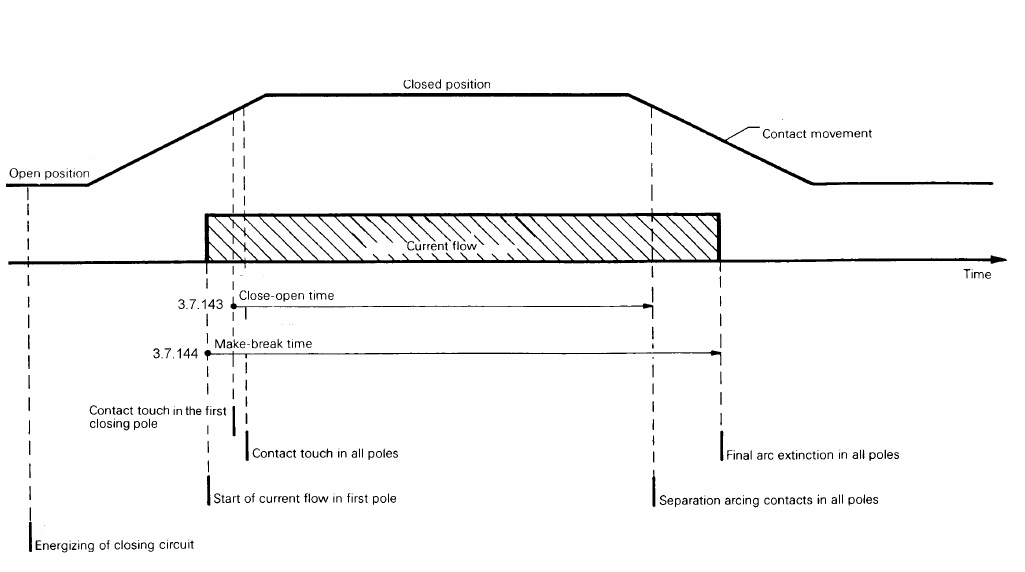
\includegraphics[width=\textwidth]{TimeDefinitionsduringCloseOpenCycleforCBwithout} 
%   \caption{Time Definitions during Close-Open Cycle for CB without Switching Resistors}
%   \label{Fig:Time Definitions during Close-Open Cycle for CB without Switching Resistors} 
%\end{sidewaysfigure}

%\begin{sidewaystable}
%    \centering
%    \caption{Your caption here}
%   \begin{tabular}{ll}
%    First First & First Second\\
%    Second First & Second Second
%    \end{tabular}
%\end{sidewaystable}
%--------------------------text subscript--------------------------------------
\usepackage{fixltx2e}

\usepackage[justification=centerlast]{caption} 
\usepackage{subcaption}
\usepackage{ragged2e}
%------------------------------- et al ----------------------------------------
\usepackage{filecontents}
%-------------------------------Degree Symbol----------------------------------
\usepackage{siunitx}
\usepackage{textcomp}

%------------Fancy Header Setting-------------------
\usepackage{fancyhdr}
\lhead{}
\chead{}
\rhead{\thepage}
\lfoot{}
\cfoot{}
\rfoot{}
\renewcommand{\headrulewidth}{0pt}
\renewcommand{\footrulewidth}{0pt}
%----------------------------- Program code -----------------------------------
\usepackage{listings}
\usepackage{courier}
%-----------------------------Java Eclips syle---------------------------------
\definecolor{javared}{rgb}{0.6,0,0} % for strings
\definecolor{javagreen}{rgb}{0.25,0.5,0.35} % comments
\definecolor{javapurple}{rgb}{0.5,0,0.35} % keywords
\definecolor{javadocblue}{rgb}{0.25,0.35,0.75} % javadoc
 
\lstset{language=Java,
basicstyle=\linespread{0.8}\ttfamily\small,
keywordstyle=\color{javapurple}\bfseries,
stringstyle=\color{javared},
commentstyle=\color{javagreen},
morecomment=[s][\color{javadocblue}]{/**}{*/},
numbers=left,
numberstyle=\footnotesize\color{black},
stepnumber=1,
numbersep=16pt,
tabsize=2,
showspaces=false,
showstringspaces=false,
breaklines=true}

%Document body
	%\begin{lstlisting}
	% Add code here
	%\end{lstlisting}
 
% Or load from file
	%\lstinputlisting{filename.java}
%--------------------------------Author and Title-------------------------------

\author{Mrs. Anita Arun Bhole}
\title{Effect of Dynamic Properties of Circuit Breaker on Short Circuit Capacity}
%--------------------------------Custom biblography------------------------------

% Define the IEEE citation control command (not necessary if using IEEEtran class)
\makeatletter
\def\bstctlcite{\@ifnextchar[{\@bstctlcite}{\@bstctlcite[@auxout]}}
\def\@bstctlcite[#1]#2{\@bsphack
  \@for\@citeb:=#2\do{%
    \edef\@citeb{\expandafter\@firstofone\@citeb}%
    \if@filesw\immediate\write\csname #1\endcsname{\string\citation{\@citeb}}\fi}%
  \@esphack}
\makeatother
%---------------------------------------------------------------------------------
%\nocite{*} %For print biblography

\begin{document}
\bstctlcite{IEEEexample:BSTcontrol}

\pagenumbering{gobble}

\begin{titlepage}
%-----------------------FRONT PAGE------------------------------------------------
\begin{center}
~\\
\textit{\small The Thesis Entitled}\\
\vspace{1cm}
\textcolor{ured}{\textbf{\large EFFECT OF DYNAMIC PROPERTIES OF CIRCUIT BREAKER ON SHORT CIRCUIT CAPACITY}}\\
\vspace{0.5cm}

\includegraphics[width=.30\textwidth]{universityLOGOf}\\
\vspace{0.6cm}
\textit{\normalsize Submitted to}\\
\vspace{0.5cm}
\textcolor{ublue}{\textbf{\large Dr. BABASAHEB AMBEDKAR MARATHWADA UNVIERSITY, AURANGABAD}}\\
\vspace{1cm}
\textit{\normalsize In partial fulfilment of the Requirement for the Award of the Degree of}\\
\textbf{\large DOCTOR OF PHILOSOPHY}\\
\textit{\normalsize in}\\
\textbf{\normalsize ELECTRICAL ENGINEERING}\\
\textbf{\textit{\small By}}\\
\textcolor{ured}{\textbf{\normalsize Mrs. Anita Arun Bhole}}\\
\textit{\normalsize Under the Guidance of}\\
\textcolor{ured}{\textbf{\large Dr. W. Z. Gandhare}}\\
\vspace{1cm}
\textbf{\normalsize FACULTY OF ELECTRICAL ENGINEERING}\\
\textbf{\large Dr. BABASAHEB AMBEDKAR MARATHWADA UNVIERSITY, AURANGABAD-431 004 (MS), INDIA\\
\colorbox{Yellow}{SEPTEMBER - 2017}}
\end{center}
\clearpage
%-------------------------SECOND PAGE------------------------------------------------------
~\\
\textcolor{ured}{\textbf{\textit{\large EFFECT OF DYNAMIC PROPERTIES OF CIRCUIT BREAKER ON SHORT CIRCUIT CAPACITY}}}
\vspace{2cm}

\textcolor{ublue}{\textbf{\large Ph. D. Thesis}}\\
\textit{\normalsize in Electrical Engineering}\\
\vspace{2.5cm}


\textit{\small Author}\\
\textcolor{ured}{\textbf{\large Mrs. Anita A. Bhole}}\\
\small Research Scholar
\vspace{3cm}

\textit{\small Under the Guidance of}\\
\textcolor{ured}{\textbf{\large Dr. W. Z. Gandhare}}\\
\vspace{0.5cm}

\small Director, G. S. Moze College of Engineering, Pune\\
\small Research Guide in Electrical Engineering\\
\small Dr. Babasaheb Ambedkar Marathwada University\\
\small Aurangabad - 431 004 (MS) INDIA
\vspace{2cm}

\colorbox{Yellow}{\textbf{\textit{\large SEPTEMBER 2017}}}
\clearpage
%-----------------------INSIDE COVER PAGE -----------------------------------------------------
\begin{center}
~\\
\textbf{\large EFFECT OF DYNAMIC PROPERTIES OF CIRCUIT BREAKER ON SHORT CIRCUIT CAPACITY}\\
\vspace{0.5cm}

\includegraphics[width=.3\textwidth]{universityLOGO}\\
\vspace{0.8cm}
\textit{\normalsize Submitted to}\\
\textbf{\large Dr. BABASAHEB AMBEDKAR MARATHWADA UNVIERSITY, AURANGABAD}\\
\vspace{1cm}
\textit{\normalsize for the Degree of}\\
\textbf{\normalsize Doctor of Philosophy}\\
\textit{\normalsize in} \\
\textbf{\normalsize Electrical Engineering}\\
\textbf{\small By}\\
\textbf{\large Mrs. Anita Arun Bhole}\\
\textit{\normalsize Under the Guidance of}\\
\textbf{\large Dr. W. Z. Gandhare}\\
\vspace{1cm}
\textbf{\large FACULTY OF ELECTRICAL ENGINEERING}\\
\textbf{\large Dr. BABASAHEB AMBEDKAR MARATHWADA UNVIERSITY, AURANGABAD-431 004 (MS), INDIA\\
\colorbox{Yellow}{SEPTEMBER - 2017}}
\end{center}

\clearpage

%-----------------------CERTIFICATE-------------------------------------------------------------
\pagenumbering{roman}
\addcontentsline{toc}{chapter}{\numberline{}Certificate}
\begin{center}
\large \textbf{Dr. Babasaheb Ambedkar Marathwada University\\
Aurangabad (M. S.) - 431 004}\\
\vspace{0.5cm}

\includegraphics[width=.3\textwidth]{universityLOGO}\\
\vspace{0.5cm}


\textbf{\large CERTIFICATE}\\
\end{center}
\normalsize This is to certify that the thesis entitled \textbf{\textquotedblleft Effect of Dynamic Properties of Circuit Breaker on Short Circuit Capacity\textquotedblright}, which is being submitted herewith for the award of the \textbf{\textquoteleft Degree of Doctor of Philosophy\textquoteright ~in \textquoteleft Electrical Engineering\textquoteright} of~ \textbf{Dr. Babasaheb Ambedkar Marathwada University Aurangabad}. This is the result of the Original Research Work and Contribution by \textbf{\textquoteleft Mrs. Anita Arun Bhole\textquoteright} under my supervision and guidance at Government College of Engineering, Aurangabad. The work embodied in this thesis has not formed earlier for the basis of the award of any degree or compatible certificate or similar title of this for any other diploma/examining body or university to the best of knowledge and belief. 

\vspace{0.5cm}
Place: \textbf{Aurangabad}\\
Date~: \textbf{~~~/~~~/}\\

\hspace{2.2in}
\begin{minipage}{4in}
\vspace{0.5in}
\begin{center}
\textbf{Dr. W. Z. Gandhare}\\
Research Guide\\
Electrical Engineering\\
Faculty of Engineering \& Technology\\
Dr. Babasaheb Ambedkar Marathwada\\University, Aurangabad\\
\end{center}
\end{minipage}

\clearpage
%-----------------------ABSTRACT-------------------------------------------------------------
\chapter*{ABSTRACT}
\addcontentsline{toc}{chapter}{\numberline{}Abstract}
Modern high voltage circuit breaker (CB) consists of two contact sets of main and arcing contacts. The main contacts are made of copper with silver coating and carry the normal current continuously without heating whereas tungsten-copper arcing contacts opens followed by main contacts and are exposed to arcing. The arcing contacts have to sustain the arc current, arc energy and the high temperature around 10,000\textdegree K. Hence arcing contacts are liable to damage due to severe thermal stresses and Transient Recovery Voltage (TRV). Damaged main and arcing contacts reduce the short circuit capacity of circuit breaker. Therefore the condition assessment of circuit breakers contact is of prime importance. Static contact resistance measurement evaluates the condition of main contacts only. The lack of direct access to the arcing contacts and use of high pressure gas complicate the direct condition assessment of this part. Hence the Dynamic Contact Resistance Measurement (DCRM) test has been recently introduced as a condition assessment test for CB main and arcing contacts. Many parameters such as length of arcing contact, contact wipe and erosion of main and arcing contacts, contact misalignments, healthiness of linkage mechanism, main and arcing contact resistance, contact travel and speed \textit{etc}. can be obtained from signature.

Switching under different fault condition and certain normal duty leads to severe TRVs across the contacts of the circuit breakers which may fail the circuit breaker to clear the fault and has the influence on the short circuit capacity of the circuit breaker. In this thesis study of TRV under different fault conditions for IEEE network is carried out and the short circuit capability of the CB is determined using computer simulations in EMTP-RV. DCRM tests and timing measurement tests are conducted on 400 kV and 245 kV SF\textsubscript{6} CBs at circuit breaker manufacturing industry, 400 kV substation Waluj, Aurangabad and 765 kV substation at Thapti Tanda Aurangabad. Data of DCRM for healthy breakers as well as breakers with problems in condition of contact was collected from the largest utility company Power Grid Corporation of India Ltd. (PGCIL) as well as Maharashtra State Electricity Transmission Company Ltd. (MSETCL). DCRM signature obtained from the test is difficult to analyze as it needs the knowledge of circuit breaker design, operating mechanism, and interrupter assembly and also expertise to conclude the cause. Numbers of case studies are presented and the measured and collected DCRM data is analyzed and a new algorithm has been proposed to detect the contact anomaly. Computer program is developed to determine the health of CB.

\clearpage

%-----------------------DECLARATION-------------------------------------------------------------
\begin{center}
\large \textbf{Dr. Babasaheb Ambedkar Marathwada University\\
Aurangabad (M. S.) - 431 004}\\
\vspace{0.5cm}

\includegraphics[width=.3\textwidth]{universityLOGO}\\
\vspace{0.5cm}
\addcontentsline{toc}{chapter}{\numberline{}Declaration}

\textbf{\large DECLARATION}\\
\end{center}

\normalsize I hereby declare that the work presented in the form of thesis entitled \textbf{\textquotedblleft EFFECT OF DYNAMIC PROPERTIES OF CIRCUIT BREAKER ON SHORT CIRCUIT CAPACITY\textquotedblright} is an original research work carried out by me under the guidance of Dr. W. Z. Gandhare, Director, G. S. Moze College of Engineering Pune, and has not been previously submitted to this or any other University for the award of degree, diploma, associate-ship, or any other similar title.

\vspace{0.5cm}
Place: \textbf{Aurangabad}\\
Date~: \textbf{~~~/~~~/}\\

\hspace{2.2in}
\begin{minipage}{4in}
\vspace{0.5in}
\begin{center}
\textbf{Mrs. Anita Arun Bhole}\\
Research Scholar
\end{center}

\end{minipage}
\clearpage
%%-----------------------EVALUATION CERTIFICATE-----------------------------------------------
%\begin{center}
%\large \textbf{Dr. Babasaheb Ambedkar Marathwada University\\
%Aurangabad (M. S.) - 431 004}\\
%\vspace{0.5cm}
%
\includegraphics[width=.3\textwidth]{universityLOGO}\\
%\vspace{0.5cm}
%
%\textbf{\large EVALUATION CERTIFICATE}\\
%\end{center}
%
%
%\normalsize \textbf{Mrs. Anita A. Bhole} has done the appropriate work for the fulfilment for the award of \textquotedblleft Degree in Philosophy\textquotedblright in \textquoteleft Electrical Engineering\textquoteright ~of Dr. Babasaheb Ambedkar Marathwada University Aurangabad (M.S.).
%
%\hspace{1cm}
%\begin{minipage}{4in}
%\vspace{0.5in}
%1.~Chairman:\\
%\\
%2.~External Referee:\\
%\\
%3.~Guide:\\
%\\
%Place: \textbf{Aurangabad}\\
%Date~: \textbf{~~~/~~~/}\\
%\end{minipage}

%\clearpage
%-----------------------ACKNOWLEDGEMENT------------------------------------------------------

\begin{center}
\large \textbf{ACKNOWLEDGEMENT}
\addcontentsline{toc}{chapter}{\numberline{}Acknowledgement}
\end{center}

\setlength{\parskip}{1em}
\justify \normalsize I take this opportunity to thank my guide Dr. W. Z. Gandhare, Director, G.S.Moze College of Engineering, Pune for his valuable guidance and constant motivation during the research work. I wish to thank Internal Monitoring Committee Members Dr. A. S. Bhalchandra, Dr. M. G. Shaikh and Dr. A. G. Thosar, Head of Electrical Engineering Department, Government College of Engineering, Aurangabad for their valuable support, suggestions and extending all the facilities for completion of this research work. I am thankful to Dr. P.B. Murnal for permitting to carry out the research work. Many thanks to my colleagues at the institute for their help and support.

I owe special thanks to the authority of Crompton Greaves, Nashik for permitting to conduct the experimentation and measurements. Also I greatly acknowledge the authorities of PGCIL and MSETCL for the technical support and permission to visit the substation and carry out the testing.

Last but not least, I express my deepest love to my family with all my heart for patience and unfailing support through the research work.

\setlength{\parskip}{0em}
\vspace{2cm}
\begin{flushright}
\textbf{Anita Arun Bhole}
\end{flushright}
\clearpage

\newgeometry{left=1.5in,right=1in,top=0.9in,bottom=0.9in}
\tableofcontents
\restoregeometry
\clearpage

\pagenumbering{roman}

\listoffigures
\addtocontents{lof}{\protect\addcontentsline{toc}{chapter}{\numberline{}List of Figures}}

\listoftables
\addcontentsline{toc}{chapter}{\numberline{}List of Tables}

\printnomenclature
\addcontentsline{toc}{chapter}{\numberline{}Abbreviations}
\end{titlepage}
%\pagestyle{fancy}

\nomenclature{ANSI}{American National Standards Association}
\nomenclature{CB}{Circuit Breaker}
\nomenclature{HVCB}{High Voltage Circuit Breaker}
\nomenclature{CBY}{Circuit Breaker Years}
\nomenclature{MaF}{Major Failure}
\nomenclature{Mif}{Minor Failures}
\nomenclature{SF\textsubscript{6}}{Sulpher Hexafluoride}
\nomenclature{TRV}{Transient Recovery Voltage}
\nomenclature{PGCIL}{Power Grid Corporation of India Ltd.}
\nomenclature{MSETCL}{Maharashtra State Electricity Transmission Company Ltd.}
\nomenclature{SCRM}{Static Contact Resistance Measurement}
\nomenclature{DCRM}{Dynamic Contact Resistance Measurement}
\nomenclature{RRRV}{Rate of Rise of Transient Recovery Voltage}
\nomenclature{IEC}{International Electro Technical Commission}
\nomenclature{IEEE}{Institute of Electrical and Electronics Engineers} % List of Abbrivations

\chapter{INTRODUCTION}
\pagestyle{fancy}
\thispagestyle{empty}
\pagenumbering{arabic}
%Introduction

\section{Introduction}
American National Standards Association (ANSI) defines the Circuit Breaker (CB) as, \textquotedblleft A mechanical switching device, capable of making, carrying, and breaking currents under normal circuit conditions and also making, carrying for a specified time, and breaking currents under specified abnormal circuit conditions such as those of short circuit\textquotedblright
 \cite{DefinitionforPower}. CBs are required to fulfil following physical requirements apart from main functions \cite{van2001transients}.

\begin{itemize}
\item Should work as a good conductor when closed and a good insulator when opened
\item Should quickly interrupt the short circuit current
\item Should not generate over voltages during switching
\item Should be highly reliable during operation
\end{itemize}

Components involved in basic functions of High Voltage Circuit Breakers (HVCBs) can be divided into five groups \cite{cigre2000user}.

\justify
\begin{description}[style=nextline, before={\setcounter{descriptcount}{0}},font=\bfseries\stepcounter{descriptcount}\thedescriptcount.~]

\item[Contacts] Contacts are the main component which should be able to carry the rated current continuously without overheating and should carry large current without welding for a short period during short circuit condition. Hence contacts are the key component in deciding the success or failure of the CB. Condition monitoring of contacts avoids the failure of this critical component.

\item[Switching] CBs are subjected to electrical, thermal and mechanical stresses during switching. It is required that CBs should be able to perform its duty under normal and abnormal conditions without causing failure. The parameters like pole mismatch, contact travel, contact wear, operating time and arcing time are used to monitor the switching of CB. 

\item[Insulation] The insulating components must be so designed as to withstand the mechanical and electrical stresses. In HVCBs solid, liquid, vacuum and gaseous dielectric materials are used to provide electrical insulation.

\item[Operating Mechanism] The function of the operating mechanism is to open and close the circuit breaker contacts within the specified limits. CBs remain in closed position for an extended period of time. But during fault condition, it has to open reliably. Hence the job of the operating mechanism is not simple. The percentage of failure of operating mechanism is large in the total failures of HVCBs.

\item[Control and auxiliary functions] Control and auxiliary components are controlled by 110-220 V DC. According to reliability surveys, control and auxiliary components are exposed to failures relatively frequently. Delay in operation or failing to open or close on demand are some typical failures in these parts.
\end{description}

\setlength{\parskip}{1em}

Renewable energy sources are being used to cater the power demand in the fast growing power systems. The reliable switching of CBs in controlling power flows and during critical contingency condition is important \cite{hedman2009optimal, kezunovic2014reliable, gu2014fast}. CBs gets deteriorated due to usage and ageing. Hence they need proper maintenance. Conventionally CBs have been maintained through time-based maintenance schedule \cite{hinow2011substation, li2004cost, razi2013priority, liu2010optimal, razi2013priorityassessment}.

In POWERGRID network failure survey was carried out. Since the CB operation is~ not~ frequent~ for~ extra high~ voltage network, manufacturers~ recommend overhauling of CB after ten years of service or at a specific number of operations. It was observed that there had been damages in the components in the interrupting chambers much before ten years where as there were few CBs with 17-20 years of age in good condition with no abnormality \cite{sodha2012condition}. Thus condition based maintenance has been reported as the most efficient to recognize the need for maintenance of CBs when necessary. It is the cost effective maintenance and ensures the reliability \cite{long2012online, gungor2012cognitive, moghe2012smart, razi2014circuit, qiang2012high}.

CIGRE has conducted three world wide surveys since 1970 on high voltage CBs reliability \cite{janssen2014international,mazza1981first,cigre1994final,cigre2012final}. The reliability is expressed in failure per 100 CB years (CBY) or per 10,000 operating cycles for the relevant failure modes. Failures are classified as a major failure (MaF or MF) and minor failures (Mf or Mif). The third enquiry included CBs of all ages and the objective was the relationship between age and major failure rate. Figure \ref{fig:Application of CBs} shows that 54\% of the total population is for the overhead line.

\begin{figure}[!htbp]
    \centering
    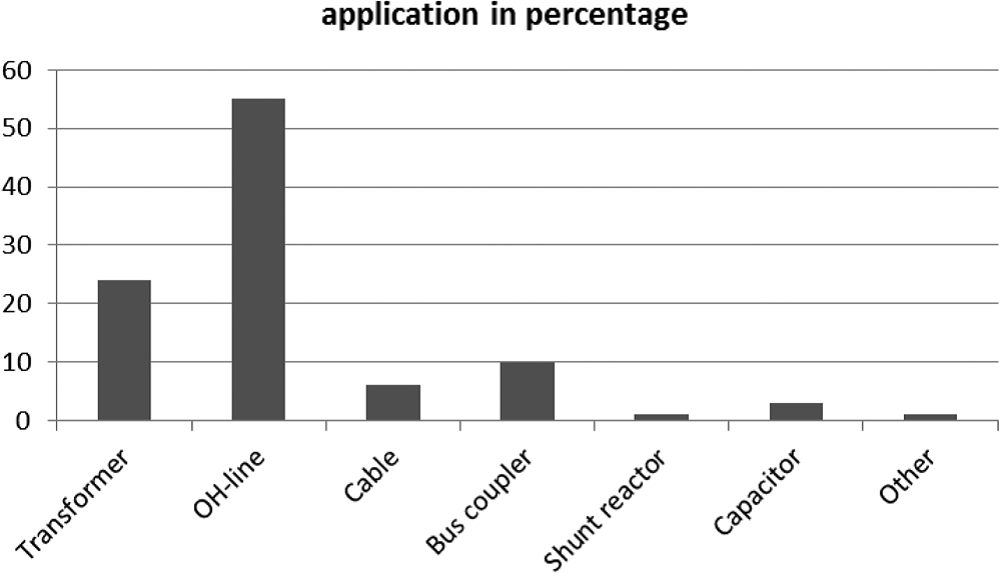
\includegraphics[width=\textwidth]{ApplicationofCBs}
    \caption[Application of CBs]{Application of CBs \cite{janssen2014international}}
    \label{fig:Application of CBs}
\end{figure}

Shunt reactors and shunt capacitor bank percentage is very less, but they cover more than 20\% of failure. The technology of operating mechanism is changing towards spring mechanism as seen in figure \ref{fig:Maf Rate per Drive Technology for Failures [18]}. Table \ref{table:Percentage of Maf Rate} shows the percentage of MaF and MiF rate per failure mode reported in the third enquiry.

\begin{figure}[!htbp]
    \centering
    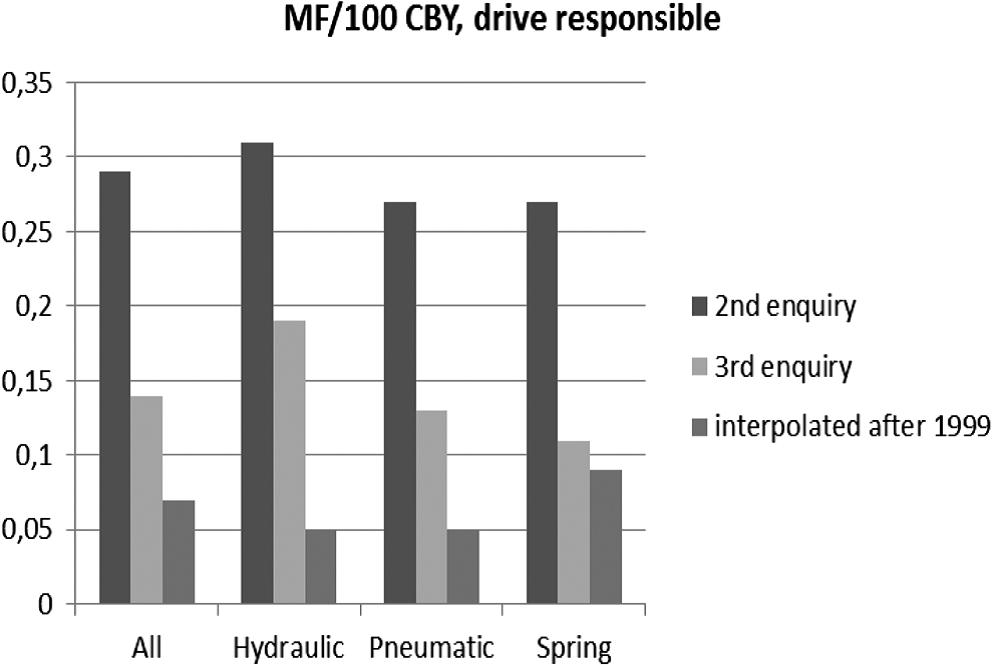
\includegraphics[width=\textwidth]{MafRateper}
    \caption[Maf-Rate per Drive Technology for Failures]{Maf-Rate per Drive Technology for Failures \cite{janssen2014international}}
    \label{fig:Maf Rate per Drive Technology for Failures [18]}
\end{figure}


\begin{table}[!htbp]
\begin{threeparttable}
\renewcommand{\arraystretch}{1.3}
\caption{Percentage of Maf Rate and Mif Rate per Failure Mode, Third Inquiry}
\label{table:Percentage of Maf Rate}
\centering
\small
\begin{tabular}{| >{\arraybackslash}m{1.9in} |>{\centering\arraybackslash}m{0.6in} |>{\arraybackslash}m{3in} |}

%\begin{tabular}{| l | c | l |}
\hline
\multicolumn{1}{|c|}{\textbf{MaF failure mode}}	&	\textbf{MaF(\%)}	& \multicolumn{1}{|c|}{\textbf{Comments}}								\\ \hline
Does not close on command	&	28.2				& Mainly with live tank circuit breakers			\\ \hline
Does not open on command	&	16.4				&													\\ \hline
Closes without command		&	0.2					&													\\ \hline
Opens without command		&	5.4					&													\\ \hline
Fails to carry the current	&	1.3					&													\\ \hline
Dielectric breakdown		&9.9					& Breakdown to earth: 5\%, Internal breakdown across open pole, during opening operation = does not break the current: 1.9\%, Other across open pole: 1.8\%, Breakdown between poles: 1.2\%					\\ \hline
Locked in open or closed position & 25.1			& Alarm has been triggered by the control system	\\ \hline
Loss of mechanical integrity&	8.1					& Mechanical damage of parts						\\ \hline
Other						&	5.2					&													\\ \hline
Total						&	100					&													\\ \hline \hline
\multicolumn{1}{|c|}{\textbf{MiF failure mode}}	& \textbf{Mif(\%)}		& \multicolumn{1}{|c|}{\textbf{Comments}}									\\ \hline
Air or hydraulic oil leakage&	20.3				& In operating mechanism							\\ \hline
Small SF\textsubscript{6} gas leakage		& 35.6					& Large leakage will give MF-mode \textquotedblleft
Locked\textquotedblright
			\\ \hline
Oil leakage in grading capacitors &	1.0				&													\\ \hline
Change in functional characteristics& 28.4			& 6.8\% mechanical; 3.3\% electrical 18.3\% control%
													  and auxiliary systems								\\ \hline
Other and no answer			& 14.6					&													\\ \hline
Total						& 100					&													\\ \hline
\end{tabular}
%\begin{tablenotes}
%\item \cmark -- functionality is available. \hspace{0.5in} \xmark -- functionality is not available.
%\end{tablenotes}
\end{threeparttable}
\end{table}

\subsection{Circuit Breaker Classification}
Figure \ref{Fig:Classification of CBs} shows the complete classification of circuit breakers. However, CBs are classified mainly according to the dielectric medium used for arc extinguishing \cite{nasrallah2007electrical}.

\begin{sidewaysfigure}
   \centering 
   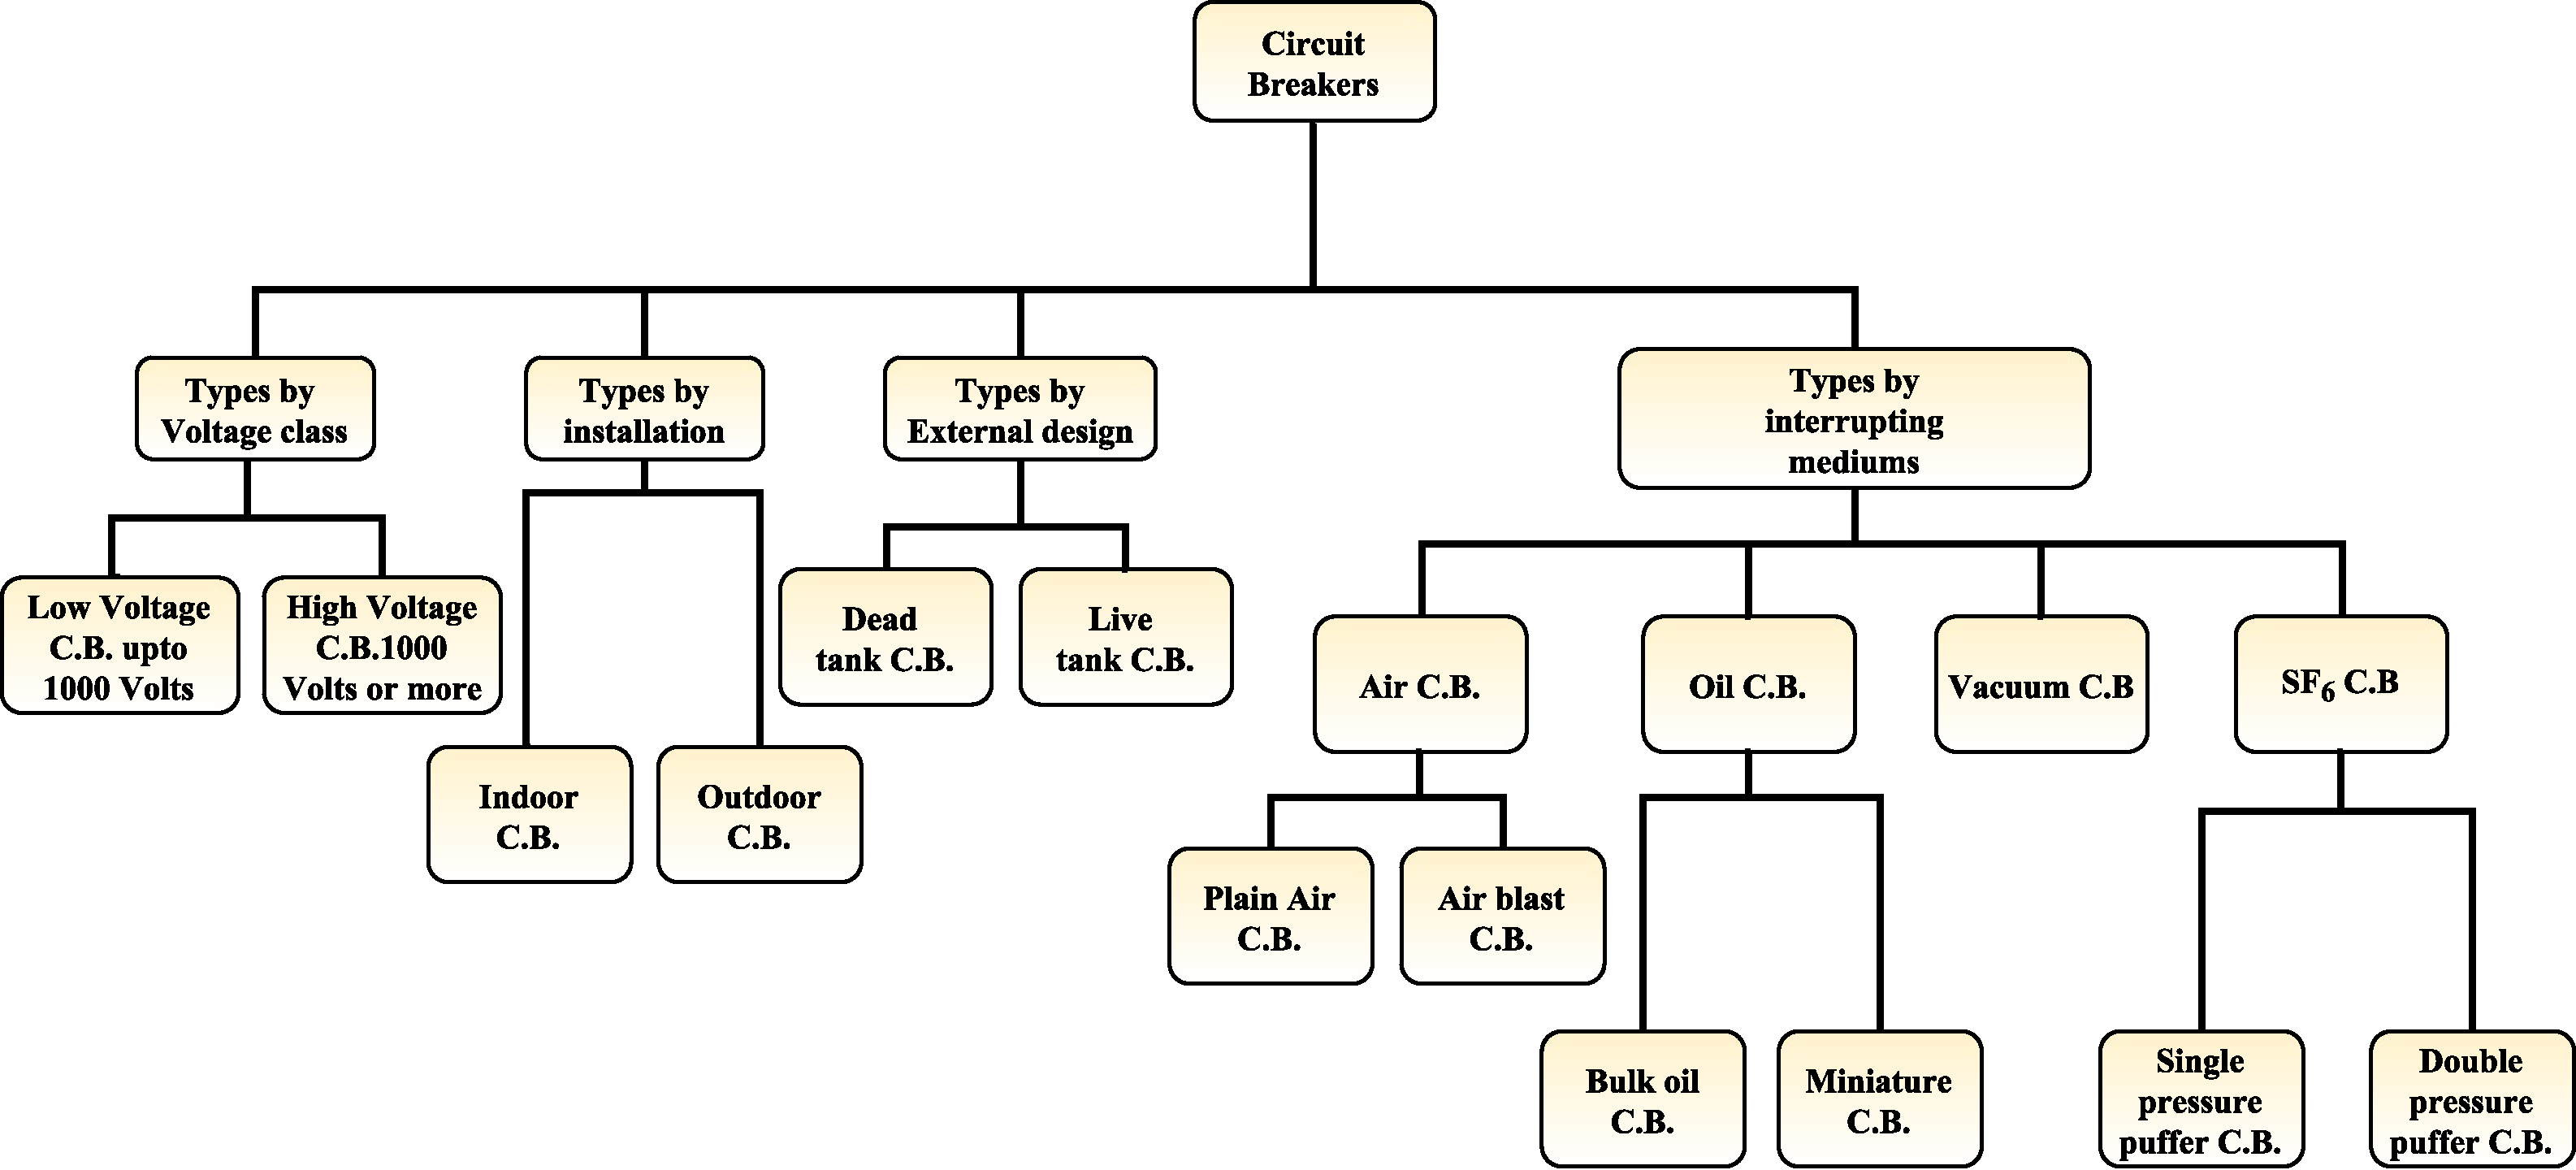
\includegraphics[width=\textwidth]{ClassificationofCBs} 
   \caption{Classification of CBs}
   \label{Fig:Classification of CBs}
\end{sidewaysfigure}

\clearpage
\section{Motivation}
The power system is growing at a faster pace. Increase in level of transmission voltage necessitates the use of HVCBs. The reliability of system depends on the CBs which has a crucial role in isolating the faults. Most of the population of circuit breakers in high voltage transmission is SF\textsubscript{6} circuit breakers. Modern high voltage puffer type SF\textsubscript{6} circuit breakers have two parallel contact sets. The low resistance silver plated main contacts carry the load current whereas the tungsten-
copper arcing contacts, which opens after the main contact are exposed to arcing. Hence arcing contacts are liable to damage due to severe thermal stresses and Transient Recovery Voltage (TRV). Damaged main and arcing contacts reduce the short circuit capacity of the circuit breaker. Therefore the condition assessment of circuit breakers contact is of prime importance.

Study of CB failures survey by CIGRE working group observed that the failures are mainly due to malfunction of the operating mechanism and control circuit. The major contribution of the fault is from aging, wear and corrosion (50\%) followed by the manufacturing faults, design faults and incorrect maintenance (15\%) \cite{janssen2014international}. Failure survey motivated to study circuit breaker condition monitoring aspects.

\clearpage
\section{Objectives}
The objectives of the proposed research work are, to:
\begin{enumerate}
\item  Study the interruption of current under three phase to ground terminal fault at the substation for multiple line switching and transformer switching and to measure the TRV and compare it with standard TRV to determine the short circuit capability of the CB

\item Study the interruption of single phase to ground short line fault and to measure the TRV and compare it with standard TRV to determine the short circuit capability of the CB

\item Measure and study~ the static contact resistance~ and~ dynamic~ contact resistance of 245 kV and 400 kV SF\textsubscript{6} CBs at the High Voltage circuit breaker manufacturing industry and in the field

\item Collect the data of DCRM for normal and abnormal cases from the PGCIL, MSETCL and High Voltage  circuit breaker manufacturing industry

\item Analyze the DCRM data and develop an algorithm to determine the wearing of main and arcing contacts, contact wipe to determine the health of CB

\item Apply the Black Box Cassie - Mayer arc model for arc interruption studies
\end{enumerate}

\clearpage
\section{Theme}
The interruption chamber of circuit breaker comprises of sets of the fixed and moving main and arcing contacts which are prone to erosion with time and usage. The lack of direct access to those and use of high-pressure gas complicate the direct condition assessment of this part. Circuit breakers need to perform various switching duties. Switching under the different fault condition and certain normal duty leads to severe TRVs across the contacts of the circuit breakers which may fail the circuit breaker to clear the fault and has the influence on the short circuit capacity of the circuit breaker. Hence the main theme of the proposed work has been to study the TRV under different fault conditions for IEEE network and determine the short circuit capability of the breaker using computer simulations in EMTP-RV. Also to measure the dynamic contact resistance of circuit breaker using the 4-wire method by injecting 100 A DC through the breaker. Measurements are recorded with a resolution of 100 $\mu s$ with a sampling frequency of 100 kHz. Figure \ref{fig:Theme of the Research Work} shows the theme of the research work and Figure \ref{fig:Normal DCRM Signature} indicates the DCRM signature. Measurements are done in the field and industry. Measured data and collected data from Power Grid Corporation of India Ltd. (PGCIL), Maharashtra State Electricity Transmission Company Ltd. (MSETCL) and High Voltage circuit breaker manufacturing industry have been analyzed in detail using HISAC Ultima test manager software. Results of analysis and simulations carried out are presented leading to conclusions and finally to new contributions. A new algorithm has been proposed to detect the contact anomaly. A computer program is developed in Java to determine the health of CB.


\begin{figure}[!htbp]
    \centering
    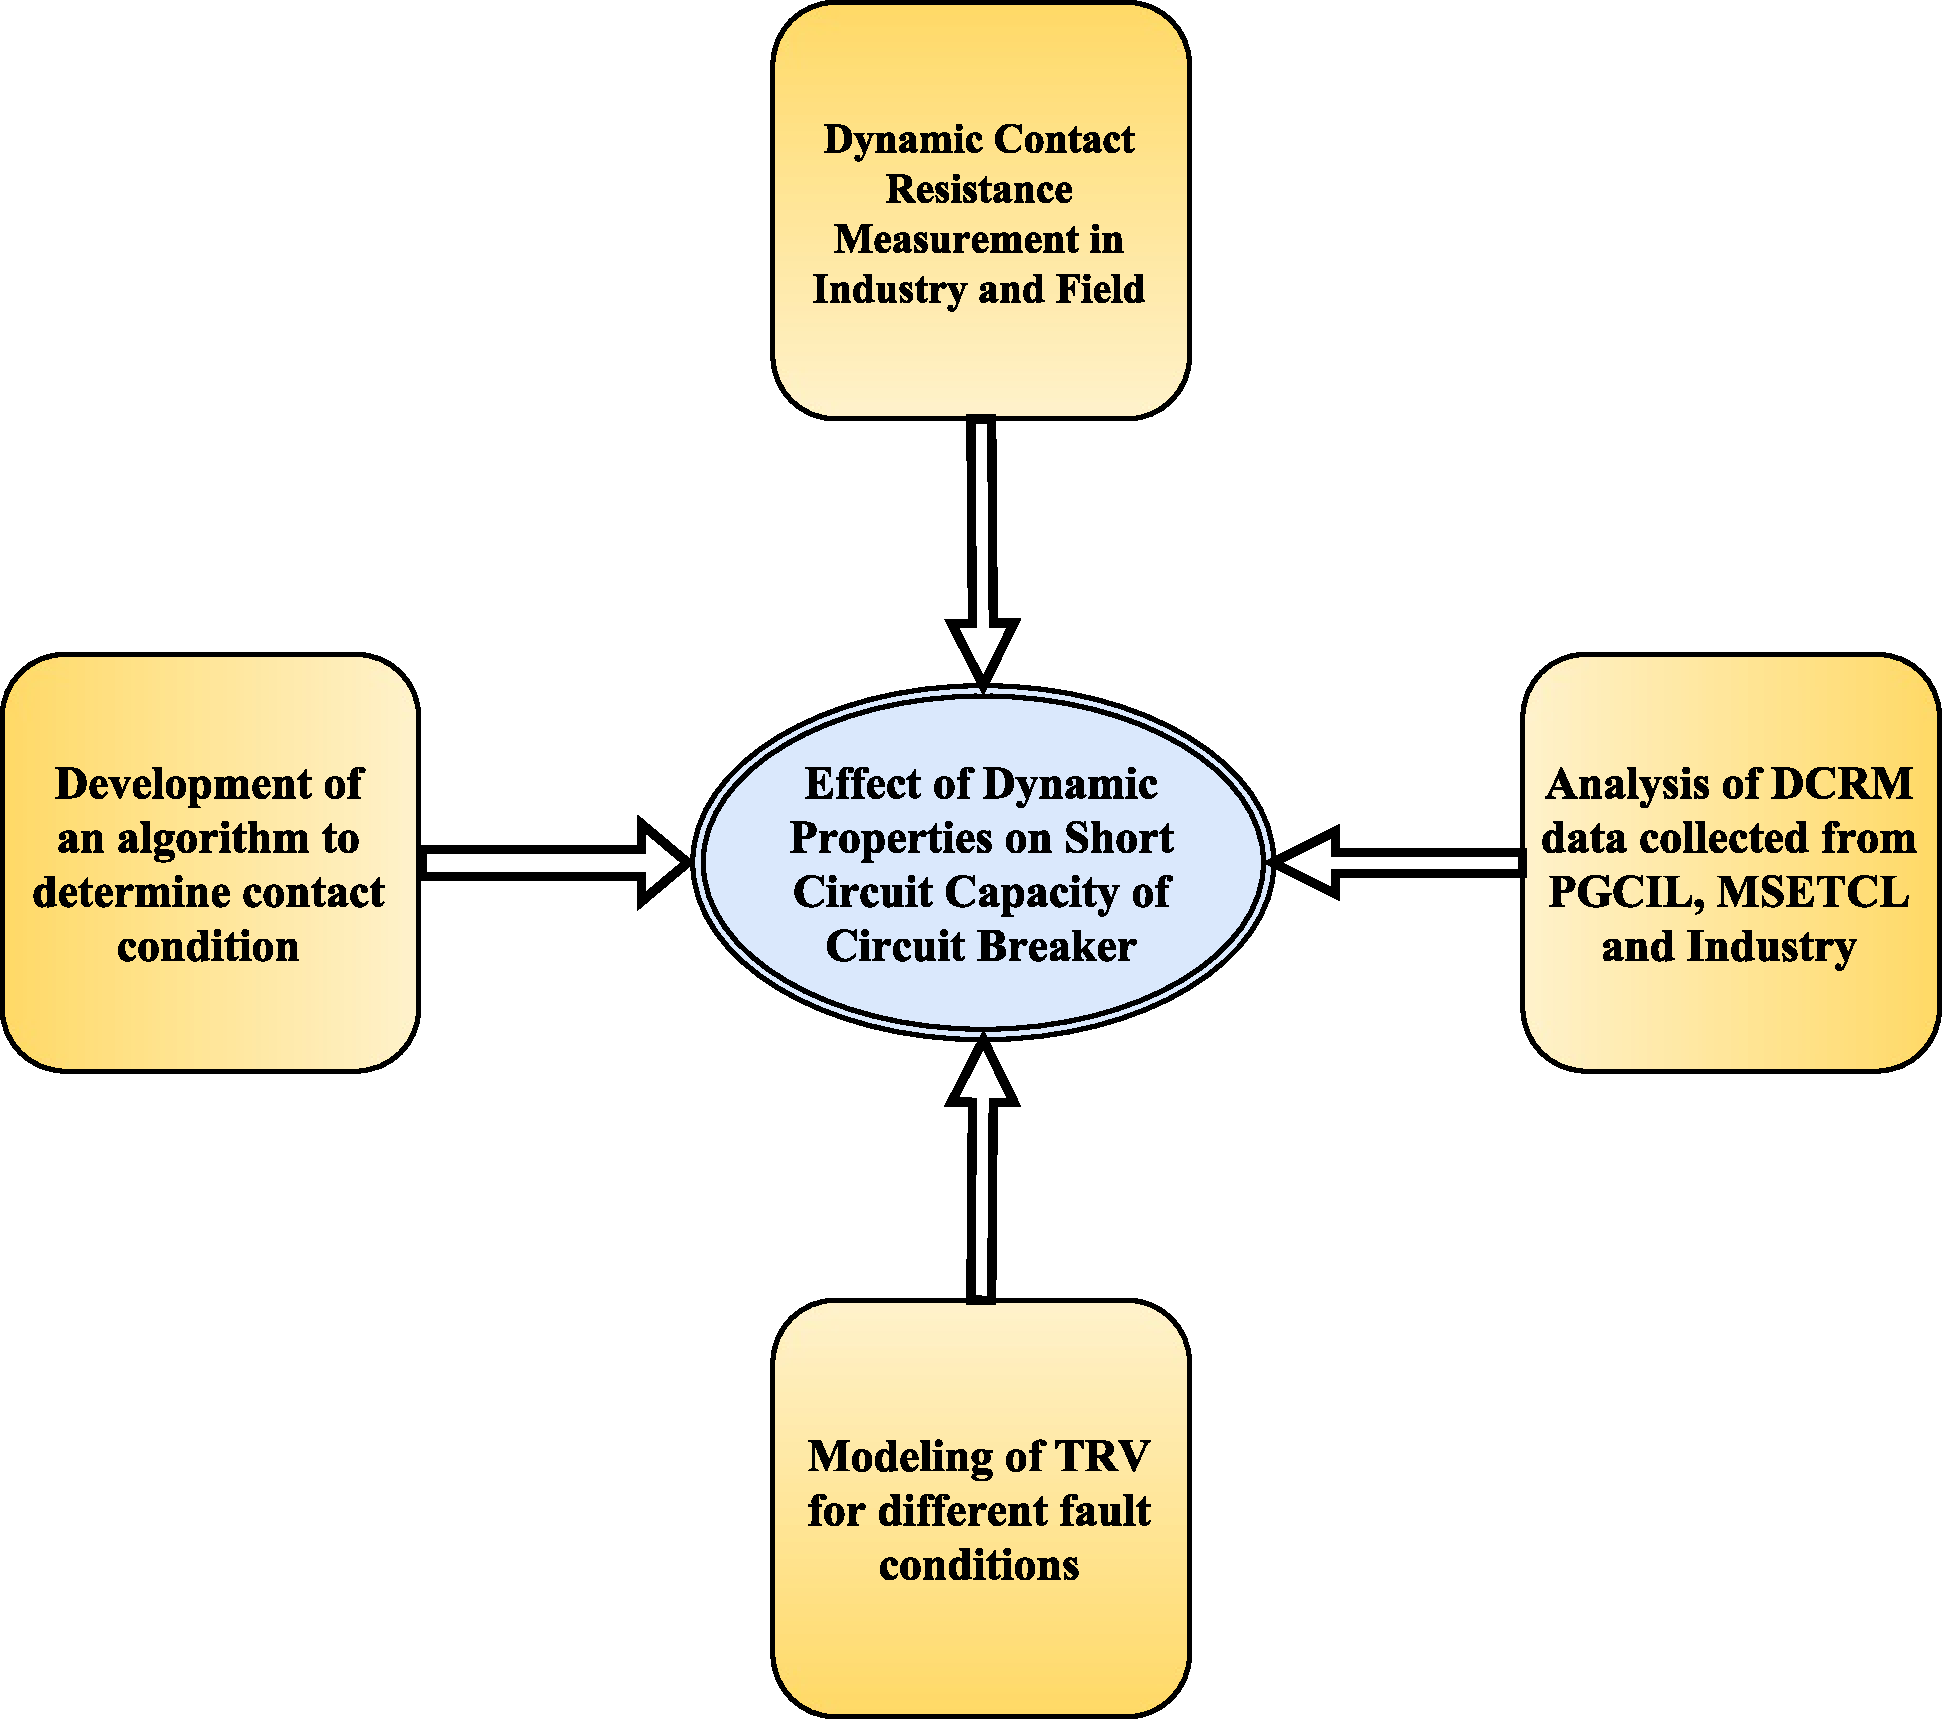
\includegraphics[width=\textwidth]{ThemeoftheResearchWork}
    \caption{Theme of the Research Work}
    \label{fig:Theme of the Research Work}
\end{figure}

\begin{figure}[!htbp]
    \centering
    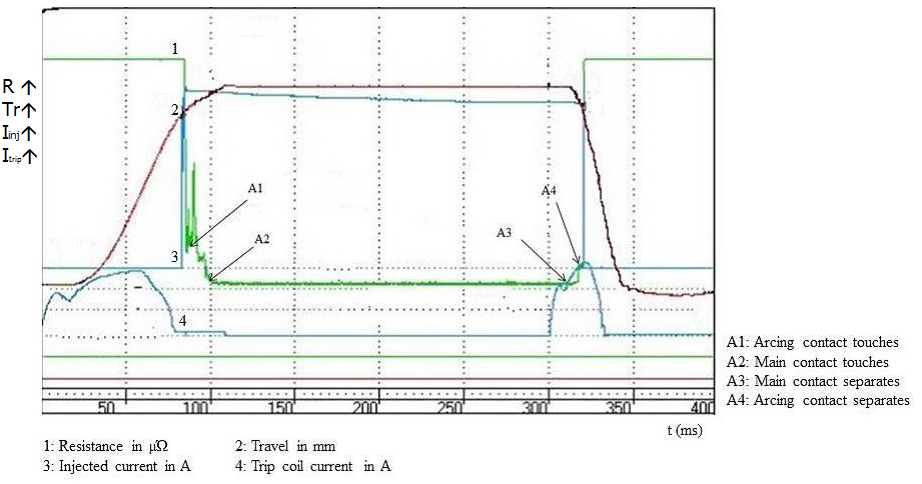
\includegraphics[width=\textwidth]{NormalDCRMSignature}
    \caption{Normal DCRM Signature}
    \label{fig:Normal DCRM Signature}
\end{figure}

\setlength{\parskip}{0em}
\clearpage
\section{Organization} 
The thesis is organized in following interdependent parts with a continuous theme as per abstract.
\subsubsection*{Chapter 1} Introduction - This chapter addresses the aspects containing introductory part. The necessity and the objectives of this research work are clearly mentioned. The overall theme of the complete research work is presented.
\subsubsection*{Chapter 2} Literature Survey - A summary of the exhaustive literature survey is represented. An overview of arc modeling, Transient Recovery Voltage, Dynamic Contact Resistance Measurement (DCRM), Standards related to circuit breaker timings are discussed in detail.
\subsubsection*{Chapter 3} System Development - Computational model of IEEE network for TRV study under different fault conditions is developed in EMTP-RV. Similarly analytical and mathematical models are developed. Dynamic contact resistance measurement is explained. Mathematical treatment is explained in detail with relevant references.
\subsubsection*{Chapter 4} Performance Analysis - Results of analytical and computational methods are presented. Justification for difference is given. Measured and collected data of DCRM from field is analyzed in detail using HISAC ULTIMA test manager software and new algorithm is proposed to detect the contact anomaly. Computer program in Java is developed to determine the health of circuit breaker.
\subsubsection*{Chapter 5} Conclusions - In this chapter conclusions of the research work, future work and  applications are presented.

\chapter{LITERATURE SURVEY}\label{chp:lit.survay}
%Literature Survey
\section{The Electric Arc}
The electric arc in a CB plays a major role in the interruption process which changes the status of breaker from conducting to a non-conducting state. An electric arc is the switching element of CB. Arc has nonlinear characteristics. The surface contact area is very small when the contacts are separated. As a result, the high current density increases the temperature that dissociates the molecules into atoms. Further increase in energy level, orbital electrons of the atoms dissociates into free moving electrons, leaving positive ions which lead to a plasma state. The Saha's equation gives the relation between the temperature T, the gas pressure P, and the fraction f of the atoms that are ionized
\begin{equation}
\frac{f^2}{1-f^2}P = 3.16 \times 10^{-7} T^{5/2} e^{-e V_i/ kT}
\end{equation}

where\\
$e ~= 1.6 \times 10^{-19}$, the charge of an electron \\
$V_i=$ ionization potential of the gaseous medium \\
$k ~= 1.38 \times 10^{−23}$, Boltzmann's constant

As shown in the figure \ref{fig:Potential Distribution Along an Arc Channel [2]}, the electric arc can be divided into three regions- the cathode region, the middle column, and the anode region. The figure also shows a potential distribution along the arc channel between the breaker contacts. The voltage drop near anode is around 5-10 volts whereas it is around 10-25 volts near the cathode region. Magnitude of arc current, length of column, types of gases and gas pressure are the parameters on which the voltage drop in the arc column depends \cite{garzon2002high}

\begin{figure}[!htbp]
    \centering
    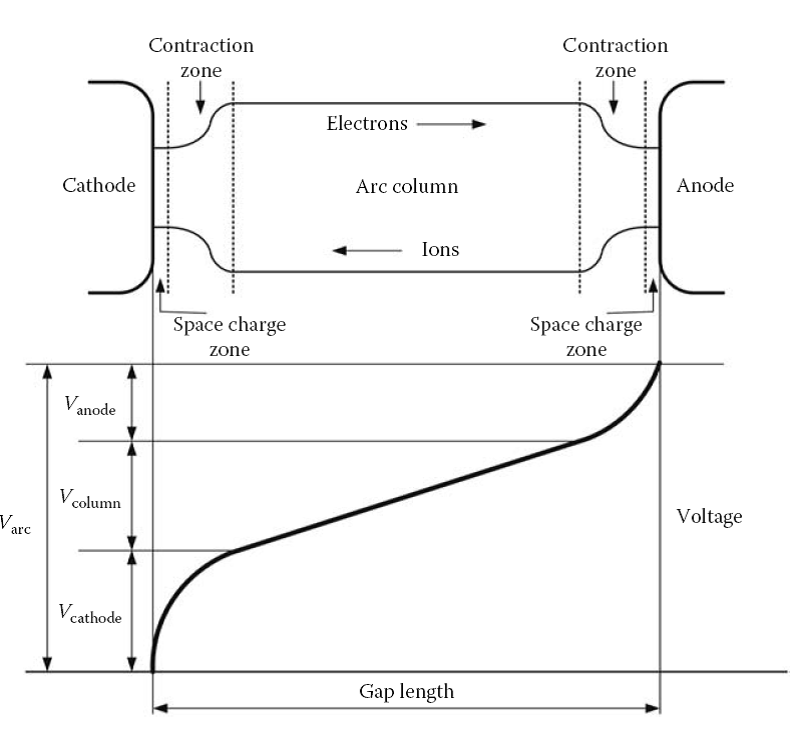
\includegraphics[width=\textwidth]{PotentialDistributionAlonganArcChannel}
    \caption[Potential Distribution Along an Arc Channel]{Potential Distribution Along an Arc Channel \cite{van2001transients}}
    \label{fig:Potential Distribution Along an Arc Channel [2]}
\end{figure}

\subsection[Time-intervals in the interruption process of an electric arc]{Time-intervals in the interruption process of an\\ electric arc}
CB is generally stressed in four intervals during fault current interruption:
\begin{itemize}
\item High current phase
\item Interaction interval
\item Dielectric recovery phase during TRV buildup
\item Dielectric withstand phase during TRV peak and recovery voltage
\end{itemize}
The intervals of CB stresses are shown in figure \ref{fig:Intervals and Failure Modes in the Interruption Process [24]}.

\begin{figure}[!htbp]
    \centering
    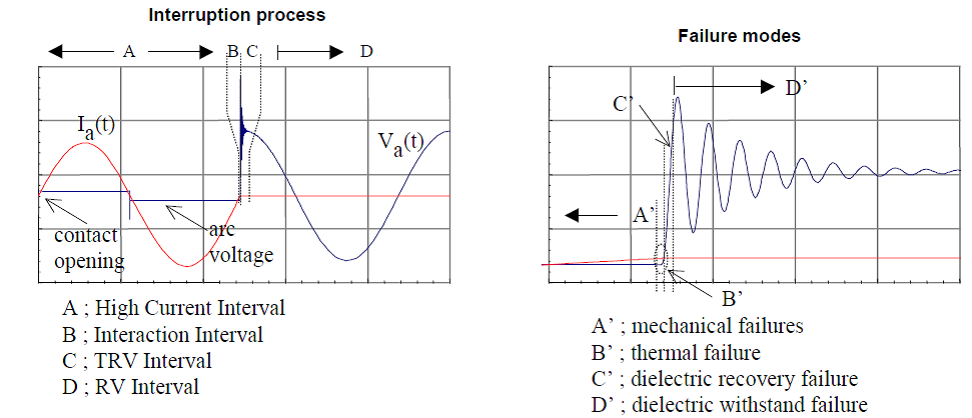
\includegraphics[width=\textwidth]{IntervalsandFailureModesintheInterruptionProcess}
    \caption[Intervals and Failure Modes in the Interruption Process]{Intervals and Failure Modes in the Interruption Process \cite{browne1984circuit}}
    \label{fig:Intervals and Failure Modes in the Interruption Process [24]}
\end{figure}

Every interval during interruption stage has specific characteristics:
\begin{itemize}
\item high volume energy input during high current phase in the arc may cause the CB to overheat or result in mechanical damage
\item possibility of reignition in interaction interval during thermal stress in arc circuit interaction
\item dielectric stress which may cause a dielectric failure of the gap between the breaker contacts during the dielectric recovery and dielectric withstand period
\end{itemize}

\section{Arc-Circuit Interaction}
Interaction of several phenomena makes the current interruption process in a high-voltage circuit breaker a complex matter. At current zero arc diameter decreases with~ the cross section~ approximately~ proportional~ to the current. ~Current interruption of the CB occurs normally at current zero. During the current interruption process strong interaction exists between the physical process between the breaker contacts and the connected network.

Figure \ref{fig:Representation of the Network Connected to the Breaker Terminals} shows the representation of the network connected to the breaker terminals.\\

\begin{figure}[!htbp]
    \centering
    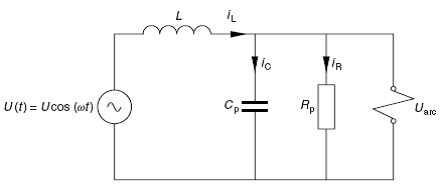
\includegraphics[width=\textwidth]{RepresentationoftheNetworkConnectedtotheBreakerTerminals}
    \caption[Representation of the Network Connected to the Breaker Terminals]{Representation of the Network Connected to the Breaker Terminals \\ \medskip \footnotesize{$L$ - Total series inductance of the network; $C_p$ - Total stray capacitance; $R_p$ - Characteristic impedance of the connected overhead lines}}
    \label{fig:Representation of the Network Connected to the Breaker Terminals}
\end{figure}

During current interruption two physical requirements are involved:
\begin{itemize}
\item Thermal regime: The hot arc channel in the arcing region has to be cooled down so that the medium stops conducting
\item Dielectric regime: The recovery voltage after the arc extinction contains high frequency transient component, Transient Recovery Voltage, which rapidly increases. The dielectric medium between the contacts must withstand this TRV for successful interruption
\end{itemize}

The current will flow for another half cycle till the next current zero if any of the above requirement is not met. Figure \ref{fig:Curves of Short Circuit Current and Recovery Voltage} shows the curves of short circuit current and recovery voltage and stresses on the extinction chamber at interruption.

\begin{figure}[!htbp]
\centering
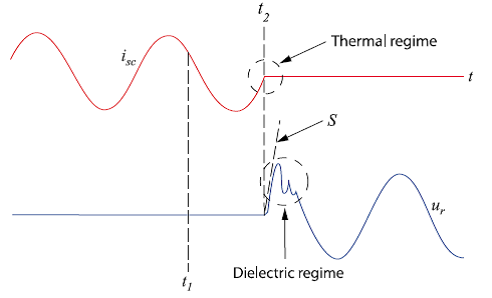
\includegraphics[width=\textwidth]{CurvesofShortCircuitCurrentandRecoveryVoltage}
\caption[Curves of Short Circuit Current and Recovery Voltage]{Curves of Short Circuit Current and Recovery Voltage \cite{Livetankcircuitbreaker}\\\medskip \footnotesize{$t_1$ - contact separation; $t_2$ - arc extinction; $S$ - rate of rise of recovery voltage}}
\label{fig:Curves of Short Circuit Current and Recovery Voltage}
\end{figure}

\subsection{Thermal regime}
\setlength{\parskip}{1em}
 The thermal regime between the CB contacts during arc interruption depends upon the initial rate of rise of the transient recovery voltage (du/dt) immediately after current zero and the rate of decrease of the current to be interrupted (di/dt). Higher values of either of these two parameters make the interruption more severe. A high value of di/dt makes the interruption difficult due to a large amount of stored energy at current zero.  High values of du/dt will result in an increase of the energy to the post-arc current. Post arc current up to few amperes flows after current zero due to electrical conductivity left in the arc path as shown in figure \ref{fig:Current Shapes at Interruption}. The successful interruption depends on the race between the energy input in the arc path by the TRV and the cooling effect.

The thermal breakdown of CB will occur if the energy input is more.

\setlength{\parskip}{0em}
\begin{figure}[!htbp]
\centering
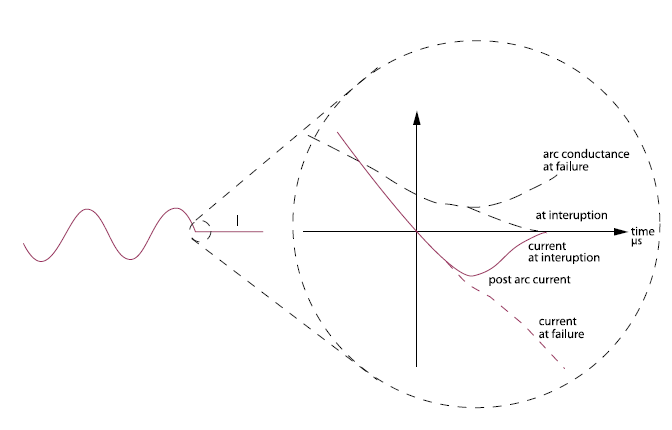
\includegraphics[width=\textwidth]{CurrentShapesatInterruption}
\caption[Current Shapes at Interruption]{Current Shapes at Interruption \cite{Livetankcircuitbreaker}}
\label{fig:Current Shapes at Interruption}
\end{figure}

\subsection{Dielectric regime}
In the dielectric regime, the temperature of the extinguishing medium is much higher than the ambient who reduce the voltage withstand capability of the contact gap. The stress on the CB depends on the Rate of Rise of Transient Recovery Voltage (RRRV). The interruption is successful if the rate of recovery of the contact gap at the instant of current zero is higher than RRRV otherwise dielectric failure will occur. Figure \ref{fig:Dielectric Interruption Regime} shows the successful and failure interruption in dielectric interruption regime.

\begin{figure}[!htbp]
\centering
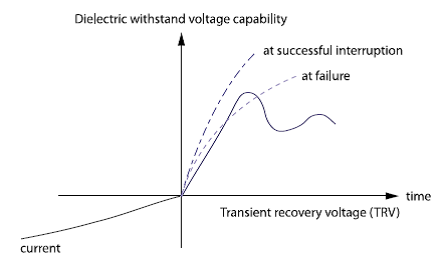
\includegraphics[width=\textwidth]{DielectricInterruptionRegime}
\caption{Dielectric Interruption Regime}
\label{fig:Dielectric Interruption Regime}
\end{figure}

\section{Circuit Breaker Modeling during Opening Operations}
CB models are needed to analyze both closing and opening operations. The separation of the contacts of the CB causes the formation of an electric arc. The main objectives of a circuit breaker model are \cite{EPRIReportEL4651}:

\begin{itemize}
\item to determine all voltages and  currents that are produced in the system due to switching action of breaker
\item to determine the reliability of CB operation under given set of conditions for the system
\end{itemize}

Modeling guidelines for CBs during closing and opening operations proposed by CIGRE WG 33-02 are shown in Table \ref{table:Modeling Guidelines for Circuit Breakers}

\begin{table}[!htbp]
\begin{threeparttable}
\renewcommand{\arraystretch}{0.9}
\caption[Modeling Guidelines for Circuit Breakers]{Modeling Guidelines for Circuit Breakers \cite{cigre199033}}
\label{table:Modeling Guidelines for Circuit Breakers}
\centering
\small
\begin{tabular}{| >{\centering\arraybackslash}m{0.5in} | >{\centering\arraybackslash}m{0.9in} | >{\centering\arraybackslash}m{0.91in} |>{\centering\arraybackslash}m{0.91in} | >{\centering\arraybackslash}m{0.91in} | >{\centering\arraybackslash}m{0.75in} |}
\hline
\multicolumn{2}{|c|}{\textbf{Operation}} & \textbf{Low-Frequency Transients} & \textbf{Slow Front Transients} & \textbf{Fast Front Transients}	&	\textbf{Very Fast Front Transients} \\ \hline
\multirow{2}{*}{Closing}& Mechanical pole spread & Important & Very important & Negligible & Negligible \\ \cline{2-6}
				 		& Prestrikes & Negligible & Important & Important & Very important \\ \hline
				 		
\multirow{4}{*}{Opening}& High current interruption & Important for interruption capability studies only & Important for interruption capability studies only & Negligible & Negligible \\ \cline{2-6}
						& Current chopping & Negligible & Important for interruption capability studies only & Important for interruption capability studies only & Negligible \\ \cline{2-6}
						& Restrike characteristics & Negligible & Important for interruption capability studies only & Very important & Very important \\ \cline{2-6}
				 		& High-frequency current interruption & Negligible & Important for interruption capability studies only &	Very important & Very important \\ \hline
\end{tabular}
\end{threeparttable}
\end{table}

\section{Arc Modeling}
\setlength{\parskip}{1em}
The design of interrupting chamber of HVCBs plays an important role in the arc interruption. Arc models were used for the better understanding of current interruption process. However, the physical phenomena involved in the current interruption is very complex. Hence it is not possible to use the arc models for CB design. However, arc models can be used for arc circuit interaction. Arc models are able to simulate the nonlinear behavior of the CB arc. Correct numerical treatment of the arc circuit problem is important due to nonlinear behavior of the arc and small time constants.

To reproduce the arc interruption phenomenon in the testing, operation, and development of CBs several approaches can be used \cite{anke1988practical}. Arc models can be classified into three categories \cite{van2001transients}.

\setlength{\parskip}{0em}
\begin{itemize}
\item Physical arc models
\item Parameter models
\item Black box arc models ( P-$\tau$ models)
\end{itemize}

\subsection{Physical arc models (PAM)}
In physical arc models, the physical process is considered in detail. The behavior of the arc is calculated from conservation laws, gas and plasma properties, and exchange mechanisms (radiation, heat conduction, turbulence). The design engineers use physical arc models for designing a new prototype. Equations \ref{eq:2.2} to \ref{eq:2.4} describe the physical arc model.

Conservation of mass:
\begin{equation} \label{eq:2.2}
\frac{\partial \rho}{\partial t} + div(\rho u) = 0
\end{equation}

Conservation of momentum:
\begin{equation} \label{eq:2.3}
\rho \frac{\partial u}{\partial t} + \rho(u \cdot grad)u = -grad(p)
\end{equation}

Conservation of energy:
\begin{equation} \label{eq:2.4}
\underbrace{\rho \frac{\partial b}{\partial t}}_{\substack{\text{change} \\ \text{of energy}\\ \text{in unit}\\ \text{volume}}}
+ 
\underbrace{u \cdot grad(\rho b)}_{\substack{\text{energy} \\ \text{input by}\\ \text{mass flow}\\ \text{convection}}}
-
\underbrace{\sigma E^2}_{\substack{\text{Joule} \\ \text{heating}}}
=
\underbrace{div(\rho u)}_{\substack{\text{work} \\ \text{performed}\\ \text{by flow}}}
+
\underbrace{div[K \cdot grad(T)]}_{\substack{\text{thermal} \\ \text{conduction}\\ \text{loss}}}
-
\underbrace{R[T, \rho]}_{\substack{\text{radiation} \\ \text{loss}}}
\end{equation}

\begin{tabular}{ >{\arraybackslash}m{3in} >{\arraybackslash}m{2.5in}}
$p$ - pressure 		 			& $\sigma$ - electrical conductivity\\
$\rho$ - gas density 			& $K$ - thermal conductivity\\
$u$ - gas flow velocity 		& $T$ - gas temperature\\
$h$ - enthalpy of gas 			& $R$ - radiation loss\\
$E$ - electric field strength	& $r$ - arc radius\\
\end{tabular}

\subsection{Black box models (BBM)}
In black box models, the arc is described by a simple mathematical equation and gives the relation between the arc conductance, arc voltage, and arc current. For arc circuit interaction in network studies, the black box models are very useful for simulation. They are based on physical considerations. The electrical behavior of the arc is important than the internal processes. In transient programs, black box models are most suitable representations \cite{anke1988practical, cigre199313}.

The aim of a black box model is to describe the interaction of the switching device and the corresponding electrical circuit during an interruption process. The aim of the Black box models is to obtain quantitatively correct performance of the CB \cite{EPRIReportEL4651}:
\begin{itemize}
\item In the simplest model the breaker is represented as an ideal switch that opens at first current-zero crossing after the tripping signal is given. This model can be used to obtain the voltage across the breaker which can be compared with a pre-specified TRV withstand capability for the breaker. This model cannot reproduce any interaction between the arc and the system

\item Arc as a time-varying resistance or conductance is used in the elaborated model. Knowledge of the initial interrupting current and breaker characteristics is used to determine the time variation. This model requires advanced knowledge of the effect of the system on the arc however the model can represent the effect of the arc on the system. Precomputed TRV curves are required to determine the adequacy of the breaker

\item  In advanced model breaker is represented as a dynamically varying resistance or conductance. The value of conductance depends on the past history of arc voltage and current. Precomputed TRV curves are not required. Generally, these models are developed to determine initial arc quenching. Some advanced models are used in determining the arc reignition in CB which occurs due to insufficient dielectric withstand capability between the breaker contacts. The effect of the arc on the system and vice versa is possible in this model
\end{itemize}

Models for representation of SF\textsubscript{6} CBs during thermal and dielectric periods were discussed and used \cite{van1992physical, van1992comparison}. Models proposed in last decades are available \cite{martinez2005parameter, avdonin1980some, maximov2009method, st1988new, schavemaker2000improved, nitu2008comparison, knobloch2001behaviour, smeets2002performance, thomas1995simulation, schavemaker1999comparison, iturregi2012considerations, karetta1998simulation, bui1997performance, liao2010study, zhang2009modelling, ziani2010application}.

\subsubsection{Cassie model}
A. M. Cassie assumed that the shape of the arc channel is a cylinder filled with an ionized gas with a constant temperature T, but with a variable diameter. It is the convection losses that govern the high current arc during the high current time interval. As the current changes, the cross section of the arc changes but the temperature inside the arc column remains constant \cite{martinez2005parameter}. For the high current region, data collected from experimental results is in good agreement with the model. However, around the current zero region, agreement is good only for high rates of current decay. Theoretically and practically, at current zero the arc diameter never decays to zero to result in arc interruption. At current zero there is a small filament of an arc remaining with a diameter of only a fraction of a millimeter. This filament is still high temperature plasma that can be easily transformed into an arc by the reappearance of a sufficiently high supply voltage. The Cassie model, in many cases, is referred to as the high current region model of an arc. This model has proved to be a valuable tool for describing the current interruption phenomena, especially when it is used in conjunction with the Mayr model.

The Cassie model is well suited for studying the behavior of the arc conductance in the high-current time interval when the plasma temperature is 8000\textdegree K or more. The Cassie model is given by equation \ref{eq:2.5}.

\begin{equation}\label{eq:2.5}
\frac{1}{g} \frac{dg_c}{dt} = \frac{1}{\tau_c} \left[\left(\frac{v}{v_0}\right)^2 - 1\right] = \frac{1}{\tau_c} \left[\left(\frac{i}{v_0g_c}\right)^2 - 1\right]
\end{equation}

\subsubsection{Mayr model}
Mayr assumed that the power losses are caused by thermal conduction at small currents, which means that the conductance is strongly temperature dependent but is independent of the cross section area of the arc. Mayr considered the arc channel to be cylindrical with a constant diameter. The model describes the arc conductance around current zero. The removal of energy from arc column is through thermal conduction. The Mayr model is suited for modeling of the arc in the vicinity of current zero when the temperature of the plasma is below 8000\textdegree K. The Mayr model is given by equation \ref{eq:2.6}

\begin{equation}\label{eq:2.6}
\frac{1}{g_m} \frac{dg_m}{dt} = \frac{1}{\tau_m} \left(\frac{v_i}{P_0} - 1\right) = \frac{1}{\tau_m} \left(\frac{i^2}{P_0g_m}- 1\right)
\end{equation}
In these equations\\ 
$g$ - arc conductance\\ 
$v$ - arc voltage\\
$i$ - arc current\\
$\tau$ - arc time constant\\
$P_0$ - steady-state power loss\\
$v_0$ - constant part of the arc voltage\\
$g_c$ is in the region of 1 $\mu s$ and $g_m$ is between 0.1 and 0.5 $\mu s$ for SF\textsubscript{6} CB.

\subsubsection{Browne model}
Mayr assumed that the arc temperature is generally above 6000\textdegree K and is likely to be in excess of 20000\textdegree K. The high temperatures lead to a linear increase of gas conductivity instead of exponential relationship. In order to take the consideration of high temperature and dynamic response representation, Mayr model must closely follow the Cassie's equation during current controlled regime. T. E. Browne recognized this need and in 1948 he developed a composite model using an equation similar to Cassie's to define the current controlled arc regime, and then converting it to a Mayr-like equation for the temperature controlled regime, and in the event that interruption did not occur at the intended current zero, he reverted again to the Cassie model. In 1958 Browne extended the application of his combined model to cover the analysis of thermal re-ignitions that occur during the first few microseconds following the critical, post current zero energy balance period. Starting with the Cassie and the Mayr equations, and assuming that before current zero the current is defined by the driving circuit, and that after current zero, the voltage applied across the gap is determined strictly by the arc circuit, Browne assumed that the Cassie equation was applicable to the high current region prior to current zero and also shortly after current zero following a thermal re-ignition. The Mayr equation was used as a bridge between the regions where the Cassie concept was applied. This model was a valuable tool that has practical applications. It has been used extensively in the design and evaluation of circuit breakers. Browne's model is given by equation \ref{eq:2.7}.
\begin{equation} \label{eq:2.7}
\frac{1}{g}= \frac{1}{g_c} + \frac{1}{g_m}
\end{equation}

\subsubsection{Avdonin model}
Avdonin proposed a model for air-blast and SF\textsubscript{6} breakers \cite{avdonin1980some}. The arc resistance of this model is expressed by equation \ref{eq:2.8}
\begin{equation} \label{eq:2.8}
\frac{dr_a}{dt}= \frac{r_a^{1-\alpha}}{A} - v_a r_a \frac{r_a^{1-\alpha-\beta}}{A B}
\end{equation}
which is derived from the modified Mayr equation \ref{eq:2.9}
\begin{equation} \label{eq:2.9}
\frac{dr_a}{dt} = \frac{r_a}{\tau} \left( 1 - \frac{v_a r_a}{P_0} \right)
\end{equation}

with

\begin{equation}
\tau = A r_a^\alpha ~~~~~~ P_0 = Br_a^\beta
\end{equation}
where\\
$r$ -  arc resistance\\
$v_a$ - arc voltage\\
$i_a$ - arc current\\
$\tau$ - arc time constant\\
$P_0$ - breaker cooling power\\

The thermal failure near current interruption and post-arc region conductivity studies are possible in this model.

\subsubsection{Urbanek model}
The Urbanek developed a model which can represent arc interruption and thermal as well as the dielectric failure \cite{maximov2009method}. Current chopping and reignition both are represented. The arc conductance is characterized by the equation \ref{eq:2.11}.
\begin{equation} \label{eq:2.11}
\frac{1}{g} \frac{dg}{dt} = \frac{1}{\tau} \left\lbrace \frac{v_i}{e^2 g} - 1 - \frac{P_0}{e^2 g} \left[ 1 - \left( \frac{v}{v_d} \right)^2 - 2 \frac{\tau}{v_d^2} v \frac{dv}{dt} \right] \right\rbrace
\end{equation}

where\\
$e$ - arc voltage for high currents\\
$P_0$ - minimum power to maintain the arc\\
$v_d$ - dielectric breakdown voltage for cold arc channel

\subsubsection{Kopplin model}
Kopplin model is used for simulation of thermal breakdown. This model is used to represent generator circuit breakers \cite{st1988new}. For the arc conductance it is characterized by a Mayr-type equation \ref{eq:2.12}
\begin{equation}\label{eq:2.12}
\frac{1}{g} \frac{dg}{dt} = \frac{1}{\tau} \left( \frac{v_i}{p_0} - 1 \right)
\end{equation}
with
\begin{equation}
\tau = K_I \cdot (g + 0.0005)^{0.25}
\end{equation}

\begin{equation}
P_0 = K_P \cdot (g + 0.0005)^{0.6}
\end{equation}

where $K_p$ and $K_I$ are model parameters.

Table \ref{table:Arc Model Applications [28]} gives the summary of applications of arc models used in the testing, development, and operation of CBs.

\begin{table}[!htbp]
\begin{threeparttable}
\renewcommand{\arraystretch}{1.3}
\caption[Arc Model Applications]{Arc Model Applications \cite{anke1988practical}}
\label{table:Arc Model Applications [28]}
\centering
\small
\begin{tabular}{| >{\arraybackslash}m{2.5in} | >{\centering\arraybackslash}m{1in} | >{\centering\arraybackslash}m{0.75in} |>{\centering\arraybackslash}m{0.75in} |}
\hline
\multicolumn{1}{|c|}{\textbf{Type of Problem}} & \textbf{Development} & \textbf{Testing} & \textbf{Operation} \\ \hline
Design optimization	&	PAM		&			&	-	\\ \hline
Mechanical system dimensioning of flow and pressure build up studies%
					&	PAM, PM	&	PAM, PM	&	-	\\ \hline
Dielectric recovery description	&	PAM, PM	&	PM	&	PM	\\ \hline
Influence of arc asymmetry and delayed current zeros	&	PAM, BBM, PM	&BBM, PM	&	PM	\\ \hline
Interruption of small inductive currents	&	PAM, BBM, PM	&	BBM, PM	&	BBM, PM	\\ \hline
Short-line fault with TRV	&	PAM, BBM, PM	&	BBM, PM	&	BBM, PM	\\ \hline
Design and verification of test circuits	&	PM	&	BBM	&	-	\\ \hline
\end{tabular}
\end{threeparttable}
\end{table}

\subsection{Parameter models (PM)}
Parameter models are basically black box models with more complex functions and tables which are derived from physical arc models and black box models.

\section{Circuit Breaker Modeling During Closing}
When the contacts of a breaker close and the gap between them get smaller, the breakdown will occur if the voltage across the gap exceeds its dielectric strength. Prestrike phenomenon during closing is shown in figure \ref{fig:Prestrike Phenomenon during Closing} \cite{martinez2009power}.

\begin{figure}[!htbp]
\centering
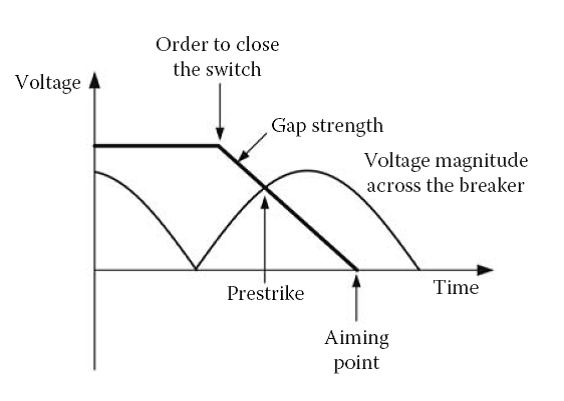
\includegraphics[width=\textwidth]{PrestrikePhenomenonduringClosing}
\caption{Prestrike Phenomenon during Closing}
\label{fig:Prestrike Phenomenon during Closing}
\end{figure}

Breaker poles closing in a multiphase breaker is random in a cycle. Hence it is difficult to determine the probability of distribution of closing time. The network on the source side or the charge trapped on transmission lines in a reclosing operation determines the peak of the transient voltages during the closing operation of CB. Instant of closing influences the maximum peak which can be different for every pole of the breaker. Many models are available to represent a CB in closing operations \cite{martinez1998digital}:
\begin{itemize}
\item In the simplest model breaker is assumed to behave as an ideal switch whose impedance changes from infinity to zero value when CB switches from open to the closing condition. The switching overvoltage across breaker depends on the closing time of breaker. For three phase system first pole to clear factor is added since all the poles do not close simultaneously. Closing instant is randomly determined in the improved approach of this model

\item In advanced approach it is assumed that there is a closing time from the instant the contacts start to close to the instant they are closed finally. Arc will strike before the contacts are completely closed if the dielectric strength of the medium is less than the withstand voltage because the withstand voltage decreases as the distance between the contacts decreases. In \cite{svensen1976influence}, pre-strike effect and its influence on the switching overvoltage during line energization is analyzed

\item  In the third approach, pre-strike dynamic arc conductance is included in the study of opening operations
\end{itemize}

\section{SF\textsubscript{6} Circuit Breakers}

\subsection{Introduction}
Figure \ref{fig:Voltage Range of Application of Breaking Technologies} shows the voltage ranges in which different breaking medium is used \cite{theoleyre1999mv}. The figure shows that SF\textsubscript{6} CBs are used in the applications for the system voltages in the range between 72.5 to 800 kV. Recently 1200 kV SF\textsubscript{6} CB is installed at Bina substation of PGCIL in Madhya Pradesh, India. Excellent dielectric strength, electron affinity or electro negativity, rapid recovery of the dielectric strength around arc region, chemically stable, non-flammable, non-corrosive, non-poisonous properties made the SF\textsubscript{6} gas superior over the other mediums used in CBs.

\begin{figure}[!htbp]
\centering
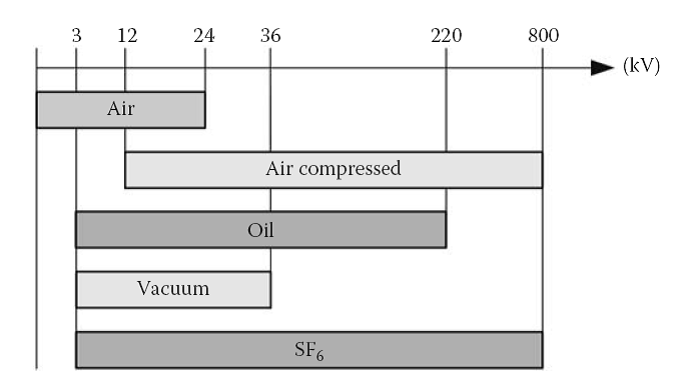
\includegraphics[width=\textwidth]{VoltageRangeofApplicationofBreakingTechnologies}
\caption{Voltage Range of Application of Breaking Technologies}
\label{fig:Voltage Range of Application of Breaking Technologies}
\end{figure}

Earlier SF\textsubscript{6} CBs were of double pressure type in which the extinguishing chamber was divided into two separate parts and were working on the principle that of air blast CBs. Nowadays puffer or self-blast principle is used for arc extinction in all high voltage SF\textsubscript{6} CBs.

\subsection{SF\textsubscript{6} puffer circuit breakers}
In the SF\textsubscript{6} puffer CBs during the opening stroke, the gas pressure for the cooling blast is created in a compression chamber. The compression of the gas will start at the same instant when the contacts start their motion during opening operation. When the arcing contacts leave the throat of the nozzle, the compressed gas is blown out along the axis of the arc. Figure \ref{fig:Main Components of the Puffer Interrupter} shows the main components of the puffer interrupter where as figure \ref{fig:Function of a Puffer Interrupter} shows its function. The current path through the closed interrupter is marked in red color.

The extinguishing pressure is current dependent in SF\textsubscript{6} puffer CBs. As seen in the no load curve figure \ref{fig:Pressure in the Puffer Cylinder at No-Load}, the maximum pressure in the puffer cylinder at no load operation is about twice the filling pressure. During a large current interruption, such as short circuit condition, gas flow through the nozzle is blocked by the arc. The arc diameter decreases during current zero which leaves more outlet area for the flow of the gas that gives maximum cooling when needed. A pressure is built up in the puffer cylinder due to blocking of the nozzle during the high current interval that may be many times the maximum no load pressure. The operating mechanism has to provide higher operating force to operate the CB due to high pressure in the puffer cylinder \cite{Livetankcircuitbreaker}.

\begin{figure}[!htbp]
\centering
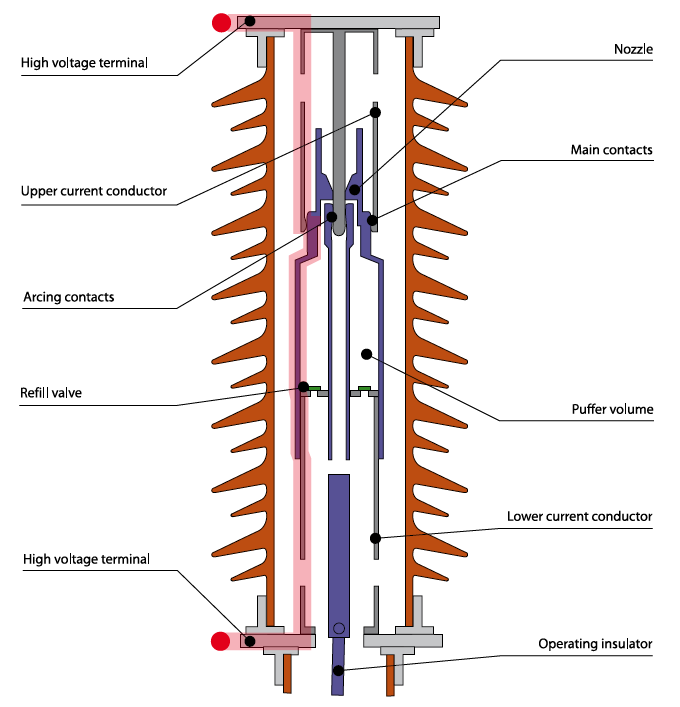
\includegraphics[width=\textwidth]{MainComponentsofthePufferInterrupter}
\caption{Main Components of the Puffer Interrupter}
\label{fig:Main Components of the Puffer Interrupter}
\end{figure}

\begin{figure}[!htbp]
\centering
\begin{minipage}{\textwidth}
\centering
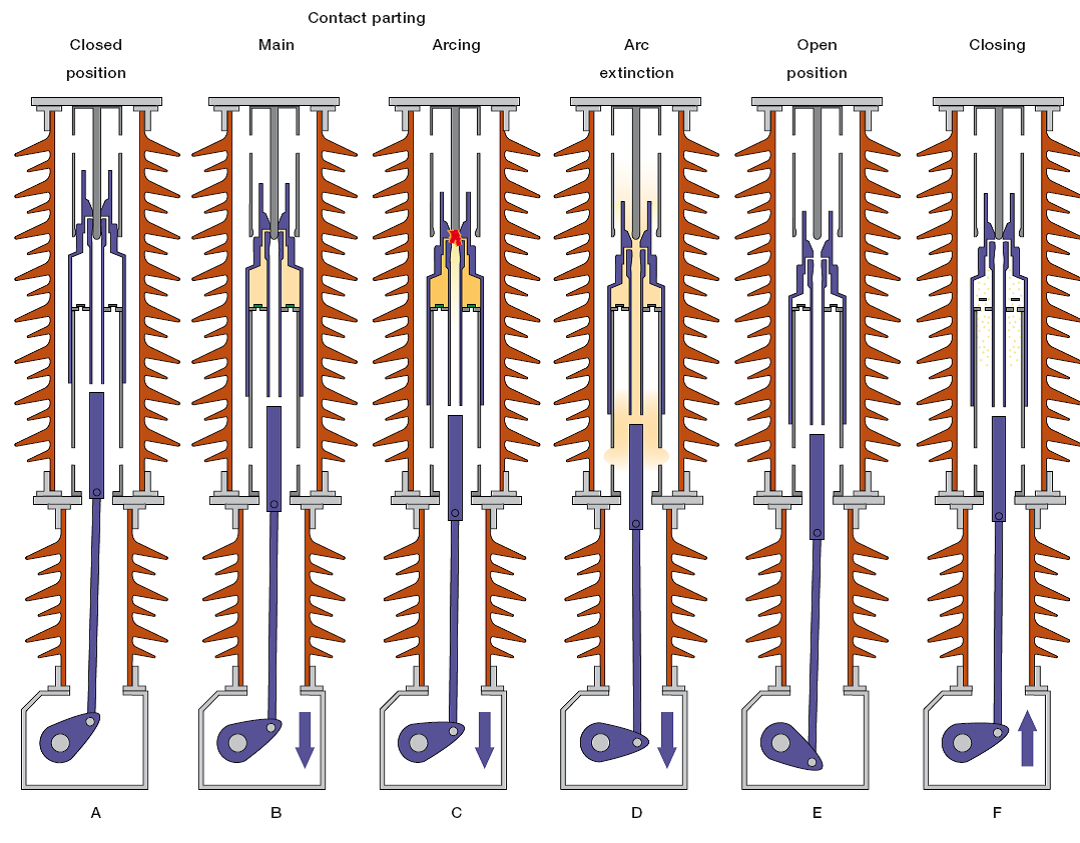
\includegraphics[width=1.1\textwidth]{FunctionofaPufferInterrupter}
\caption{Function of a Puffer Interrupter}
\label{fig:Function of a Puffer Interrupter}
\begin{flushleft}
\footnotesize A - Closed position. Current conduction through the main contacts.\\B. Main contacts separation. Starting of the moving contacts separated the main contacts commuting the current to the arcing contacts.\\C. Arc is established due to separation of arcing contacts. Pressure in the puffer cylinder starts to increase.\\
D. Arc extinction. The cold gas from the puffer volume moves rapidly through the nozzle during current zero, cooling and extinguishing the arc.\\
E. Contacts fully open.\\
F. Closing operation. Puffer volume is filled with cold gas making the interrupter ready for the next operation.
\end{flushleft}
\end{minipage}
\end{figure}

\begin{figure}[!htbp]
\centering
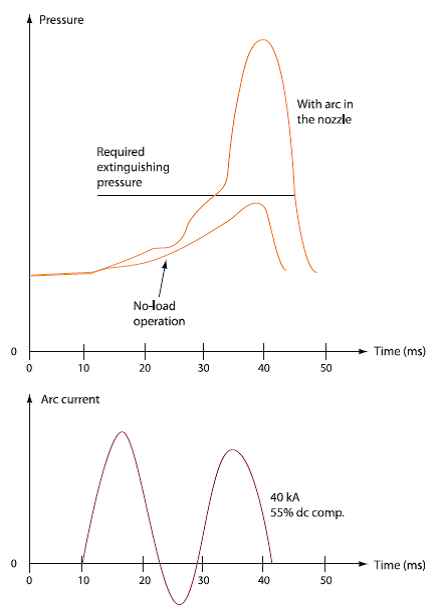
\includegraphics[width=\textwidth]{PressureinthePuffer}
\caption{Pressure in the Puffer Cylinder at No-Load and during Interruption of an Asymmetrical Short-Circuit Current of 40 kA}
\label{fig:Pressure in the Puffer Cylinder at No-Load}
\end{figure}


\subsection{SF\textsubscript{6} self-blast circuit breakers}
Most of the CB failures are of mechanical nature \cite{AlternatingCurrentCircuit}. Hence the reliability of the operating mechanism is of utmost important. In the normal puffer CB, energy from the operating mechanism is used to create the blast pressure. Self-blast principle reduced the operating energy. The arc extinction chamber in self-blast SF\textsubscript{6} CBs is divided into puffer volume and self-blast volume by the self-blast valve. During high fault current interruption, the pressure generated by the arc in the self-blast volume will be high. This high pressure closes the valve and prevents the gas from escaping into the puffer volume. The pressurized gas flows through the nozzle extinguishing the arc. But while interrupting no load current or small currents of few kA, the energy produced by the arc is insufficient to generate the pressure to close the valve. In this situation the interrupter than works as puffer interrupter.

\section{Transient Recovery Voltage}
The power system response to current interruption generates the TRV. TRV is the algebraic sum of the source side voltage and the load side voltage as shown in figure \ref{fig:Illustration of the Sources of TRV}. The shape of the TRV depends on the circuit to interrupted, characteristics of the network connections and the type of fault.

\begin{figure}[!htbp]
\centering
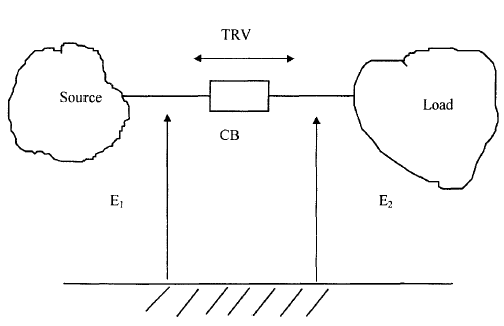
\includegraphics[width=\textwidth]{IllustrationoftheSourcesofTRV}
\caption[Illustration of the Sources of TRV]{Illustration of the Sources of TRV \cite{garzon2002high}}
\label{fig:Illustration of the Sources of TRV}
\end{figure}

IEEE and IEC both specify the standard TRV by the same approach. 
\begin{itemize}
\item The two parameters representation is used for HVCBs with a rated voltage up to 100 kV, figure \ref{fig:IEC Two and Four Parameter Limiting TRV Curves}

\item Four parameters representation is used for the CBs with rated voltage 100 kV and above, figure \ref{fig:IEC Two and Four Parameter Limiting TRV Curves}
\end{itemize}


\begin{figure}[!htbp]
\centering
\begin{minipage}{\textwidth}
\centering
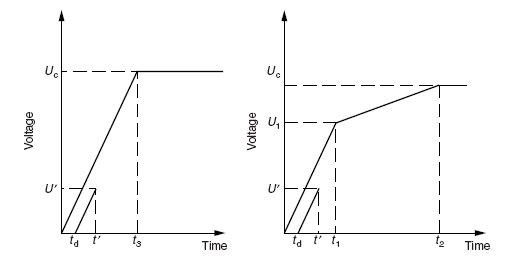
\includegraphics[width=\textwidth]{IECTwoandFourParameterLimitingTRVCurves}
\caption[IEC Two and Four Parameter Limiting TRV Curves]{IEC Two and Four Parameter Limiting TRV Curves \cite{ApplicationofTransientRecovery}}
\label{fig:IEC Two and Four Parameter Limiting TRV Curves}
\begin{flushleft}
\footnotesize \textbf{For two parameters method:}\\
$U_c$ - reference voltage, TRV peak value (kV)\\
$t_3$ - time to reach $U_c$ ($\mu s$)\\
\textbf{For four parameters method:}\\
$U_1$ - first reference voltage (kV)\\
$t_1$ - time to reach $U_1$ ($\mu s$)\\
$U_c$ - second reference voltage (TRV peak value) (kV)\\
$t_2$ - time to reach $U_c$ ($\mu s$)\\
For delay line:\\
$U^\prime$ - reference voltage (kV)\\
$t^\prime$ - time to reach $U^\prime$ ($\mu s$)\\
$t_d$ - time delay ($\mu s$)
\end{flushleft}
\end{minipage}
\end{figure}
 
The procedure and calculations necessary to apply TRV ratings for ac high-voltage circuit breakers rated above 1000 V are demonstrated in the IEEE Standard C37.011-2011 \cite{ApplicationofTransientRecovery}.

\subsection{Reactive equipment switching duty}
Switching of reactive equipment such as capacitor bank and shunt reactor is supposed to be a severe duty for CB that causes a high rate of rise of TRV across the CB contacts \cite{GuideforShuntReactorSwitching}. The high percentage of failure of CB is recorded for reactor switching and capacitor switching \cite{janssen2014international}. The inrush current during switching of isolated capacitor bank as well as back to back capacitor switching is recognized in the standards \cite{GuideforCapacitanceCurrentSwitching}. Investigations and field experience of the failure of SF\textsubscript{6} CB in the switching of 420 kV shunt reactor is presented \cite{bachiller1994operation}.  The switching transient of the shunt reactor is a high frequency response which is influenced by the surrounding circuit conditions. Figure \ref{fig:Shunt Reactor Equivalent Circuit} shows the shunt reactor equivalent circuit.

\begin{figure}[!htbp]
\centering
\begin{minipage}{\textwidth}
\centering
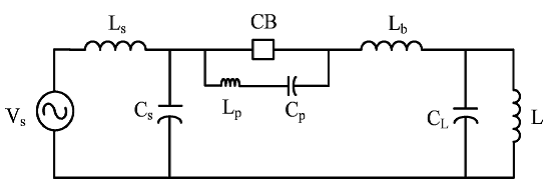
\includegraphics[width=\textwidth]{ShuntReactorEquivalentCircuit}
\caption{Shunt Reactor Equivalent Circuit}
\label{fig:Shunt Reactor Equivalent Circuit}
\begin{flushleft}
\footnotesize $L_s$ - source side inductance; $C_s$ - source side capacitance; $L_p$ and $C_p$ - stray inductance and capacitance between CB contacts; $L_b$ - the connecting series inductance; $C_L$ - load side capacitance; $L$ - shunt reactor inductance
\end{flushleft}
\end{minipage}
\end{figure}

The CB is stressed by TRV after current interruption. Reignition will take place during interruption if the contact gap is small. The reignition leads to several modes of current oscillations. These oscillations are superimposed on the reestablishing of load current and may produce current zeros at which CB will attempt to interrupt. If new interruption takes place during the first, second or main oscillation modes, then the load side oscillation starts again. Due to energy transfer between the source and load sides, the oscillating energy may change. A new reignition may occur close to the recovery peak, and if the energy has increased, the reignition voltage may be higher than at the first reignition. This procedure may be repeated several times giving multiple reignitions with an increase in voltage magnitude.
	
\subsubsection{First parallel oscillations}
Oscillations are occurring in the current through the circuit-breaker immediately after a reignition. Oscillation due to the energy source in the capacitances of direct vicinity of the circuit breaker is first parallel oscillation. These oscillations are in addition to oscillations caused by the parameters already connected in the system and parallel to them. These oscillations depend on the inherent \textquotedblleft
stray\textquotedblright capacitances of the circuit breaker pole and the few meters of conductors connected \cite{Impulseandswitchingsurge}.  In first parallel oscillation electrostatic energy stored in Cp is dissipated through the CB with no exchange between the source and load sides. The frequency of this oscillation is given by equation \ref{eq:2.15} which is of the order of 1 to 10 MHz. The CB will not interrupt the current associated with the first parallel oscillation.

\begin{equation}\label{eq:2.15}
F_{P1} = \frac{1}{2 \pi \sqrt{L_P C_P}}
\end{equation}

\subsubsection{Second parallel oscillations}
The second parallel oscillation includes the elements CS, CL, and LP. The voltage across CS and CL are equalized, \textit{i.e.} for an instant voltage across the CB is reduced to zero. The CB may interrupt the current associated with second parallel oscillation. The frequency of second oscillation, which is in the range of 50 to1000 kHz, is given by equation \ref{eq:2.16}

\begin{equation}\label{eq:2.16}
F_{P2} = \frac{1}{2 \pi} \sqrt{\frac{C_L + C_S}{L_S C_L C_S}}
\end{equation}

\subsubsection{Main circuit oscillations}
The components which relate to main circuit oscillation are: generator, capacitances and lumped inductances of the supply and load side network. Frequency is in the range of 5 to 20 kHz. During the main circuit oscillation, all circuit elements are involved, and the energy exchange is both electromagnetic and electrostatic.

\subsubsection{Source side oscillations}
 If the CB does not interrupt the current in second parallel oscillation and if the TRV is higher than the strength of dielectric recovery voltage, the oscillation is extended to source side circuit and is termed as main circuit oscillation given by equation \ref{eq:2.17} frequency of which is in the range 1 to 20 kHz. This oscillation involves the total circuit and generally leads to a new loop of current.

\begin{equation}\label{eq:2.17}
F_m = \frac{1}{2 \pi} \sqrt{\frac{L_S + L}{L_S L (C_S + C_L)}}
\end{equation}

\subsubsection{Load side oscillations}
Load side oscillation with trapped energy oscillating between the inductance and capacitance of the load side circuit during successful interruption is given by the equation \ref{eq:2.18}. The frequency is in the range of 1 to 5 kHz.

\begin{equation}\label{eq:2.18}
F_L = \frac{1}{2 \pi \sqrt{L C_L}}
\end{equation}

Figure \ref{fig:Oscillation modes in reactor circuit} shows the oscillation modes occurring in the reactor circuit \cite{chang2007modeling}.

\begin{figure}[!htbp]
\centering
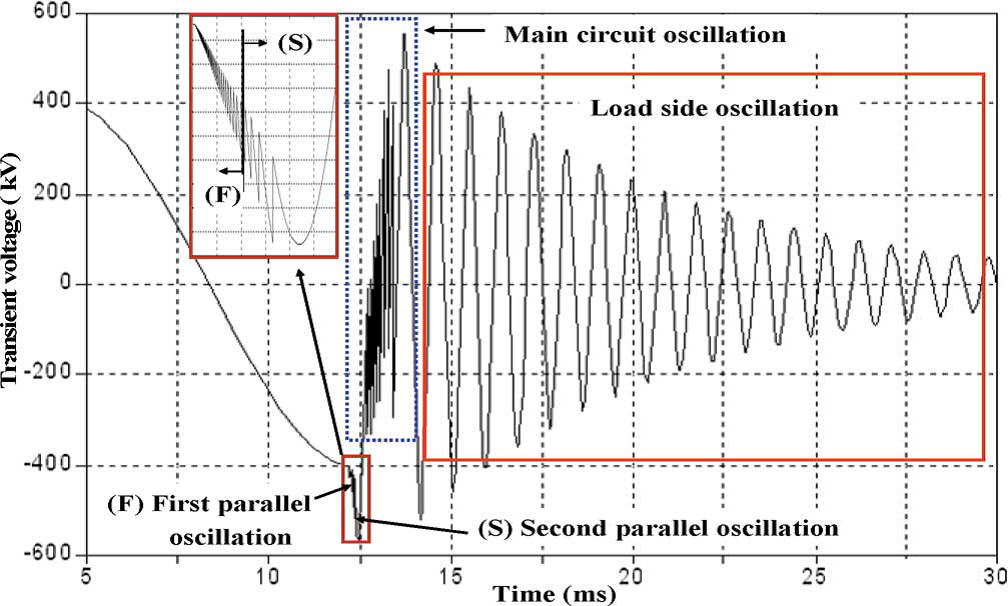
\includegraphics[width=\textwidth]{Oscillationmodesinreactorcircuit}
\caption[Oscillation Modes in Reactor Circuit]{Oscillation modes in reactor circuit \cite{chang2007modeling}}
\label{fig:Oscillation modes in reactor circuit}
\end{figure}

Circuit breaker interrupter failure is reported due to restrike which punctured right through the nozzle between the moving main contact and the fixed arcing contact of the interrupter \cite{lopez2007analysis}.

\section{Time Definitions as per IEC}
The Standard IEC 62271-100 \cite{AlternatingCurrentCircuit} covers the standard operating procedures for ac circuit breakers used for indoor or outdoor operation at 50 Hz and 60 Hz on the system having voltages above 1000 V. The most frequently used time definitions are -

\begin{description}[style=nextline]

\item[opening time] opening time is the interval of time between the instant of energizing the opening release, and the instant when the arcing contacts have separated in all poles, the circuit-breaker being in the closed position

\item[arcing time] interval of time between the instant of the first initiation of an arc and the instant of final arc extinction in all poles

\item[break time] interval of time between the beginning of the opening time of a mechanical switching device and the end of the arcing time

\item[closing time] the circuit-breaker being in the open position, closing time is the interval of time between energizing the closing circuit and the instant when the contacts touch in all poles

\item[make time] the circuit-breaker being in the open position, make time is the interval of time between energizing the closing circuit and the instant when the current begins to flow in the first pole

\item[pre-arcing time] during a closing operation, pre-arcing time is the interval of time between the initiation of current flow in the first pole and the instant when the contacts touch in all poles for three-phase conditions and the instant when the contacts touch in the arcing pole for single-phase conditions

\item[close-open time] interval of time between the instant when the contacts touch in the first pole during a closing operation and the instant when the arcing contacts have separated in all poles during the subsequent opening operation
\end{description}

Figures \ref{fig:Time Definitions during Opening and Closing, As Per IEC} to \ref{Fig:Time Definitions during Close-Open Cycle for CB without Switching Resistors} show the time definitions during opening and closing and close-open cycle respectively.

\begin{figure}[!htbp]
\centering
\begin{minipage}{\textwidth}
\centering
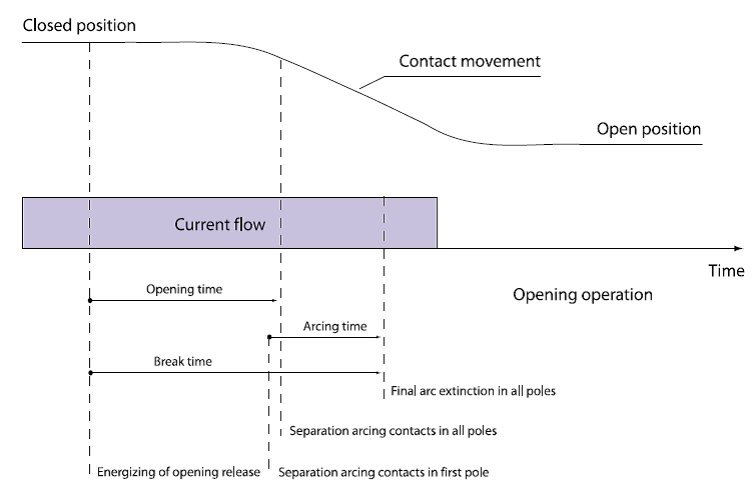
\includegraphics[width=\textwidth]{TimeDefinitionsduringOpeningandClosing1}
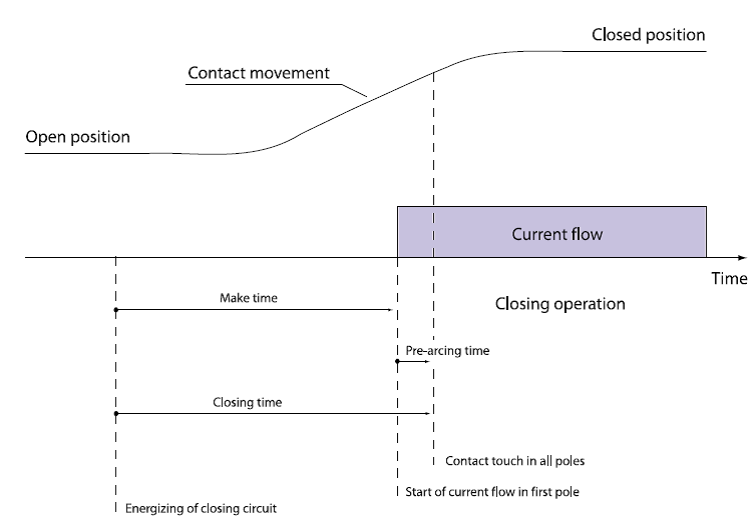
\includegraphics[width=\textwidth]{TimeDefinitionsduringOpeningandClosing2}
\caption{Time Definitions during Opening and Closing, As Per IEC}
\label{fig:Time Definitions during Opening and Closing, As Per IEC}
\end{minipage}
\end{figure}

\begin{sidewaysfigure}
   \centering 
   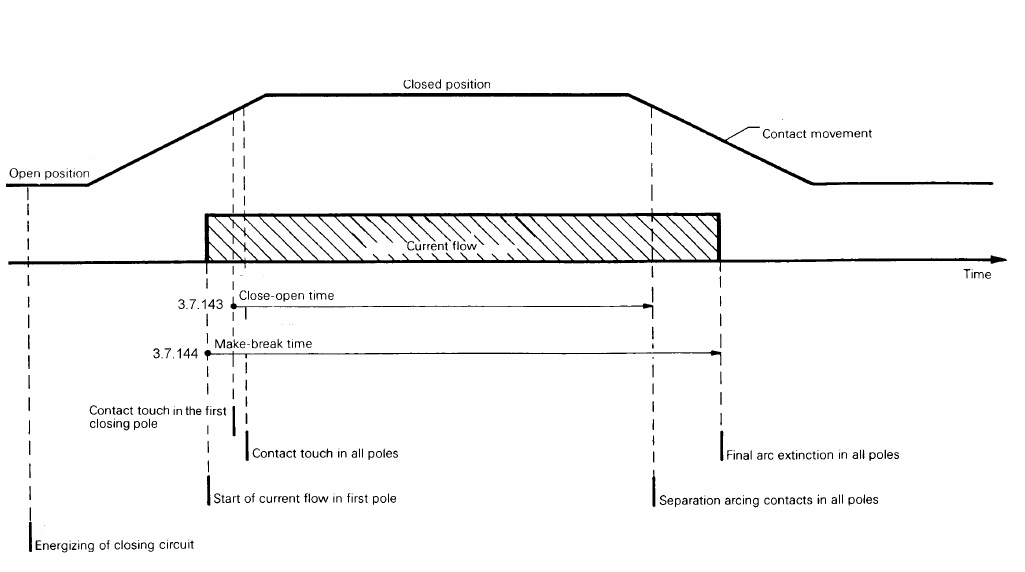
\includegraphics[width=\textwidth]{TimeDefinitionsduringCloseOpenCycleforCBwithout} 
   \caption{Time Definitions during Close-Open Cycle for CB without Switching Resistors}
   \label{Fig:Time Definitions during Close-Open Cycle for CB without Switching Resistors} 
\end{sidewaysfigure}

\subsection{Contact resistance measurement}

\subsubsection{Static contact resistance measurement (SCRM)}
Condition monitoring of CB through coil current signature, operational timings, tank gas pressure and the temperature is found \cite{dehghanian2014circuit, johal2008coil, natti2011assessing, guan2013assessing, biswas2015real, razi2015data }. However, coil current analysis does not give any information about contact condition. Generally, static contact resistance measurement is done to assess the condition of contacts. CB contacts are closed, and a DC current is passed through the contacts. IEC and ANSI recommend a value of 50A and 100A respectively. The voltage drop across the contacts is measured. The measured voltage drop, when divided by current, gives the resistance of main contacts. However, this method of resistance measurement evaluates the condition of main contacts only \cite{landry2006new}.

\subsubsection{Dynamic contact resistance measurement}
The condition of the arcing contacts is important from the point of short circuit current \setlength{\parskip}{1em} interruption capability of CB. It can be done by opening the CB interruption chamber. But this is time consuming and expensive due to high pressure SF\textsubscript{6} gas in the chamber. Also, reassembly of the unit may lead to new problems. DCRM is an indirect method of determining the condition of arcing contacts. It is quite similar to static contact resistance measurement with a difference that instead of a single value of resistance, a curve of resistance Vs time or distance is measured. Figure \ref{fig:Flow Chart of DCRM} gives the flow chart of DCRM. Close- open command is given to the CB and 100A DC current is injected. The instantaneous value of voltage and current is measured when CB opens. Resistance is calculated at each point. A curve of resistance Vs time is called as DCRM signature. DCRM signature along with the contact travel can be used to measure the main contact wipe, arcing contact wipe, average main contact and arcing contact resistance.

DCRMs during closing operations are not useful as the sudden change from infinity to the arcing contact resistance is difficult to measure. Also, undesired noise gets generated at the arcing contact touch \cite{landry2008complete}. Several spikes are observed in the DCRM curve due to partial contact separation for the CBs operated with a high speed of contact movement \cite{salamanca1993preventive, tyagi2001condition, ohlen1995dynamic}.

\setlength{\parskip}{0em}
\begin{figure}[!htbp]
\centering
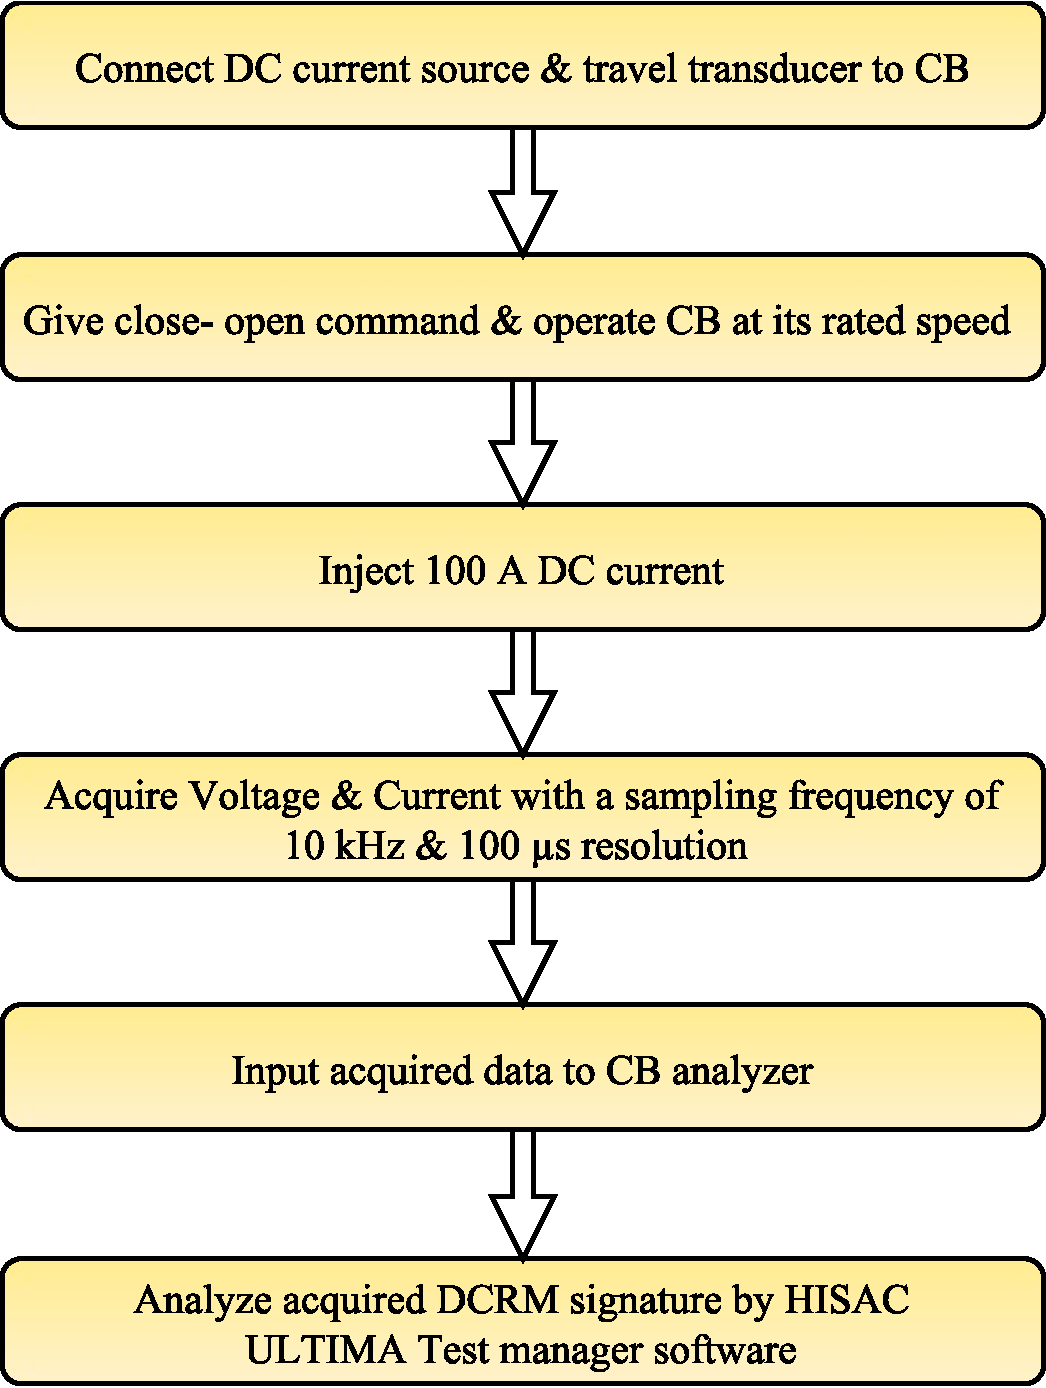
\includegraphics[width=\textwidth]{FlowChartofDCRM}
\caption{Flow Chart of DCRM}
\label{fig:Flow Chart of DCRM}
\end{figure}

\setlength{\parskip}{1em}
\textbf{Measurement at low speed}\\
M. Landry \textit{et al}. \cite{landry2006new} observed that the DCRM curves at rated speed are not comparable. The identification of main contact part was difficult. High contact speed was the reason anticipated for partial contact part. DCRMs at low speed were found identical. It was observed that the DCRM curves were smooth and the main contact parting was easy to identify. However, for some breaker mechanism, it is time-consuming to do the adjustments of a mechanism for low-speed operation. The CBs in the field are operated at rated speed. Hence the operation at low speed may not give the correct information of contacts.

\textbf{DCRM in the presence of metallic fluorides}\\
Due to arcing metallic fluorides are formed which get deposited on the CB contacts in the form of nonconductive dust powder. The effects of metallic fluorides on contact resistance have been dealt in \cite{tyagi2001condition}. High contact resistance was observed for the CB used for capacitor bank switching and which has performed a large number of operations. However, the deposition of metallic fluorides did not affect the short circuit capacity of CB. If the scraping or wiping action in the CB contact is not proper, then the high contact resistance will appear \cite{landry2006new}. Conventional equipment was used to perform the static contact resistance measurement at 100 A DC current. A high value of the contact resistance of the order of 4500-6000 $\mu \Omega$ was measured which could be interpreted as defective contacts. Michel Landry \textit{et al.} developed a method to determine the reason for high resistance which does not require the opening of CB interrupting chamber. Three current sources were connected in parallel to deliver 2800 A DC current. For carrying this high current from source to the breaker, six 4/0 copper cables were used. A measuring shunt of 51.32 $\Omega$ along with data acquisition system was used for recording the signals. Breaker contacts were kept in closed condition, and contacts were heated for different intervals in order to vaporize the metallic fluorides that were deposited on the CB contacts. DCRM were recorded for each phase at different currents. From this experimentation Michel Landry \textit{et al}. observed that heating of contacts for 15 minutes at 2800 A current reduced the arcing contact resistance to the acceptable level \cite{landry2008complete}.

\textbf{Measurement at low speed}\\
The conventional DCRM system needs heavy and long cables to connect the current source to the breaker. Ultra capacitors as a current source are discussed \cite{stanisic2010new}. The ultra capacitors along with constant charger are light weight as compared to batteries and are capable of generating few hundred amperes. A low resistance meter based on a large value of capacitor with a very small value of internal resistance, charger for the capacitor and control along with measurement circuitry for 250 A DC current was developed. The developed low resistance meter can be used for static as well as dynamic resistance measurements.

A DCRM system was developed using a stationary battery of 12V/220Ah  \cite{de2014characterization}. DCRM parameters that are useful in contact diagnosis are discussed.

A power grid experience of DCRM of CBs from PGCIL is shared \cite{sodha2012condition}. DCRM signatures of CBs from field with problems in contacts are described.

Erosion of arcing contact takes place during every operation of CB depending on the breaking current. The erosion of arcing contacts leads to the time difference between contact separations in successive operation. The contacts need the overhaul when the overlap time falls below a defined minimum value \cite{DynamicResistanceMeasurement}. 

On line monitoring of contact electrical erosion of CBs based on the theory of accumulative effect and the statistical average is developed \cite{fujie1998diagnosis}. 

High frequency DC/DC converter as a power source for generating high DC current and measuring the dynamic contact resistance of the CB is presented \cite{engineerdynamic}. 

Principal component analysis is used to get the information from dynamic resistance signal \cite{khoddam2016electrical}. 

Scoring and weighting techniques and health index are applied to identify the healthy, needs maintenance and risky condition of CB \cite{khoddam2016performance}.

Design and development process of control, acquisition, and analysis of the DCRM results for high voltage circuit breaker is presented \cite{obarvcanin2015design}.

Use of Arduino platform in measuring and processing the dynamic contact resistance curve is described \cite{de2014system}. However, it has the limitation of the sampling rate.

Testing of 400 kV CB in high induction environment is presented \cite{alibavsic2016new}. To overcome the induction voltage in recorded signal, grounding on both sides of HVCB is suggested.

All the work described in above papers focus on the measurement process of dynamic contact resistance. Methodology to detect the contact failure through DCRM is not discussed in the literature. Since the interrupter is sealed, it is not feasible to detect the contact condition. Intentional failure and then correlating the DCRM signature is not possible. 
\setlength{\parskip}{0em}

\section{Research Gap}
\setlength{\parskip}{1em}
Literature survey reveals that condition based maintenance has been the most efficient maintenance strategy. Lot of work has been done on the coil current analysis. Coil current signature can be acquired during the switching operation, and various approaches are available to determine the real time health of control circuit. Another crucial part of the circuit breakers is the main and arcing contacts.

It is observed that papers on Dynamic Contact Resistance Measurement focus on the measurement process of dynamic contact resistance. Methodology to detect the contact failure through DCRM is not discussed in the literature. Since the interrupter is sealed, it is not feasible to detect the contact condition. Intentional failure and then correlating the DCRM signature is not possible. 

The Dynamic Contact Resistance Measurement was developed around 20 years ago to assess the condition of arcing contacts without dismantling the breaker, and in India, the utility companies are using this test for condition monitoring from last ten years.

Arc formation and the TRV at the arc interruption of every CB connected to the same system configuration will be different. This is due to design aspect of CB. Hence every CB has a unique signature. Knowledge of CB design such as types of contacts, mechanism, the principle used in arc extinction, \textit{etc}. is necessary. Hence the signatures obtained from Dynamic Contact Resistance Measurement (DCRM) are difficult to interpret and may lead to wrong decisions about the condition of contacts. Signature analysis of circuit breaker for dynamic resistance measurement is developing. It is an emerging area for research.
\setlength{\parskip}{0em}

\chapter{SYSTEM DEVELOPMENT}
%system developement

Study of parameters affecting short circuit capacity of the circuit breaker is divided in:
\begin{enumerate}
\item Modeling of system for TRV studies under different fault conditions
\item Modeling of system under different fault conditions for arc interruption studies
\item Measurement of Dynamic Contact Resistance of CBs and analysis of collected DCRM signature data
\end{enumerate}

\section{Computational Models}
\subsection{Interruption of Three Phase to Ground fault}
A model of IEEE network is developed in EMTP-RV. As shown in figure \ref{fig:IEEE Network under Study }, the system consists of local sources and remote sources connected through transmission lines. Four transmission lines and two transformers supply the 145 kV station. Details are shown in figure \ref{fig:IEEE Network under Study }. Stray capacitances of equipments are also considered. The system is studied for Three Phase to Ground fault at the terminal of station for multiple lines switching and transformer switching. Breaker rating of 30 kA maximum current interruption capacity is selected for the study. Current in the steady state through fault is found out. Accordingly standard TRV is built. TRV through simulation is compared with standard TRV provided by application guide. The ability of fault interruption capability of CB is found out.

\subsection{Interruption of Single  Phase to Ground fault}
The network is further studied for Single Phase to Ground short line fault at 4.2 km from station for 16 km line. The lines are modeled in constant parameter mode as well as frequency dependent mode TRV through simulation is compared with standard TRV provided by application guide for both frequency dependent and constant parameter line model. The ability of fault interruption capability of CB is found out.

\begin{figure}[!htbp]
    \centering
    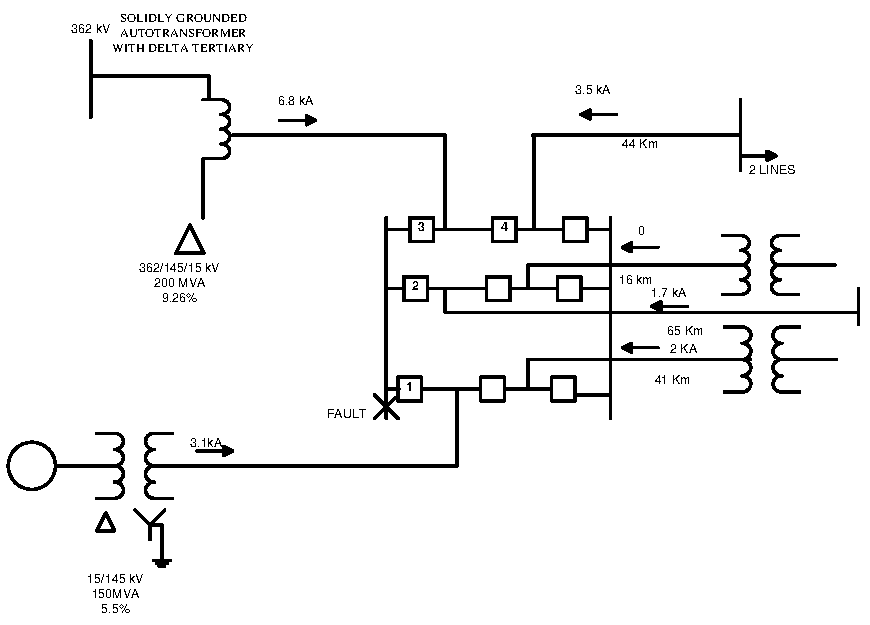
\includegraphics[width=\textwidth]{onelinediagram}
    \caption[IEEE Network under Study]{IEEE Network under Study \cite{ApplicationofTransientRecovery}}
    \label{fig:IEEE Network under Study }
\end{figure}

\subsubsection*{Parameters of the model}

\textbf{1. Local Source 1}\\
L-L RMS Voltage - 362 kV\\
Resistance - 0.16 $\Omega$\\
Inductive Reactance - 16.2 $\Omega$\\
\clearpage

\textbf{2. Transformer}\\
Nominal Rating - 200 MVA\\
L-L RMS Primary Voltage - 362 kV \\
L-L RMS Secondary Voltage - 145 kV\\
Connection type - Yg-Yg\\
Winding Resistance - 0.0009 pu\\
Winding Reactance - 0.0926 pu\\

\textbf{3. Generator Transformer}\\
Nominal Rating - 150 MVA\\
L-L RMS Primary Voltage - 15 kV \\
L-L RMS Secondary Voltage - 145 kV\\
Connection type - DYg+\ang{30}\\
Winding Resistance - 0.0005 pu\\
Winding Reactance - 0.055 pu\\

\textbf{4. Local Source 2}\\
L-L RMS Primary Voltage - 15 kV\\
Resistance - 0.002 $\Omega$\\
Inductive Reactance - 0.209 $\Omega$\\

\textbf{5. Transmission Line}\\
L-L RMS Voltage - 145 kV\\
Positive Sequence Resistance - 0.01$\Omega$\\
Zero Sequence Resistance - 0.1 $\Omega$\\
Positive Sequence Surge Impedance - 350 $\Omega$\\
Zero Sequence Resistance - 560 $\Omega$\\
Propagation Speed - 1.9 $\times$ 105 m/s\\
Length of lines - 44 km, 16 km, 65 km , 41 km\\

\clearpage

\textbf{6. Parameters of lines for frequency dependent model}\\

\begin{tabular}{ | >{\centering\arraybackslash}m{0.7in} | >{\centering\arraybackslash}m{0.7in} | >{\centering\arraybackslash}m{0.7in} | >{\centering\arraybackslash}m{0.7in} | >{\centering\arraybackslash}m{0.7in} | >{\centering\arraybackslash}m{1.2in} |} \hline
Phase & DC resistance & Outside diameter & Horizontal distance & Vertical distance &	Vertical distance at mid span  \\
{~} & $\Omega$ & (m)& (m)& (m)& (m) \\ \hline
1	& 0.126 & 0.12	&-8	&	20	&	20 \\ \hline
2	& 0.126	&0.12	&0	&	20	&	20 \\ \hline
3	& 0.126	&0.12	&8	&	20	&	20 \\ \hline
0	& 3		&0.08	&-6	&	26	&	26 \\ \hline
0	& 3		&0.08	&6	&	26	&	26 \\ \hline
\end{tabular}

~\\
\textbf{7. Arc parameters}\\
$\tau_m$ = 0.5 E-06\\
$P_0$ = 10.0 E+04\\
$\tau_c$ = 1E-06\\
$U_C$ = 2000\\
$g_0$ = 5E+07\\
$t_{trip}$ = 20 E-03\\

\section{Analytical Models}

\subsection{Transient Recovery Voltage types}
Three phase terminal fault is the most severe fault used to define the breaker rating. However, for the transmission voltages, the probability of occurrence of three phase terminal fault is very low. Hence the three phase to ground faults are the basis for rating the CB. Short line faults have lower crest magnitudes, but they have high RRRV.

\subsubsection{Three phase terminal fault}
The circuit showed in Figure \ref{fig:Circuit for Interruption of a Three-Phase-to-Ground Fault} defines the electrical equivalent network for the first phase to clear during the interruption of a three-phase terminal fault. The corresponding one-line diagram representation is shown in Figure \ref{fig:Single Line Diagram}, while Figure \ref{fig:Three Phase Diagram} indicates the three-phase representation. The reduced simple parallel RLC circuit is shown in the equivalent circuit given by Figure \ref{fig:Equivalent Circuit}. The equivalent components are given by

Equivalent inductance
\begin{equation}\label{eq:3.1}
L_{eq} = \frac{3 L_0 L_1}{L_1 + 2 L_0}
\end{equation}

In effectively grounded systems, for three-phase-to-ground faults \textit{i.e.}, with first pole-to-clear factor equal to 1.3; $L_{eq} = 1.3 L_1$.

In ungrounded systems ($L_0$ infinite), for three-phase-to-ground faults \textit{i.e.}, with first-pole-to-clear factor equal to 1.5; $L_{eq} = 1.5 L_1$

Equivalent surge impedance
\begin{equation}\label{eq:3.2}
Z_{eq} = \frac{3}{n} \times \frac{Z_0 Z_1}{Z_1 + 2 Z_0}
\end{equation}
where\\
$Z_0 = 1.6 Z_1$\\
$Z_{eq} = 1.14 Z_1 / n $\\

Equivalent capacitance
\begin{equation}\label{eq:3.3}
C_{eq} = \frac{C_0 + 2 C_1}{3}
\end{equation}

where\\
$Z_1$ - positive-sequence surge impedance of the transmission lines\\
$Z_0$ - zero-sequence surge impedance of the transmission lines \\
$n$ - number of lines\\
$L_1$- positive-sequence inductance, of all other parallel sources terminating at the station \\
$L_0$ - zero-sequence inductance, of all other parallel sources terminating at the station\\
$C_1$ - positive-sequence capacitance\\
$C_0$ - zero-sequence capacitance

For three-phase ungrounded faults on effectively grounded systems:\\
$L_{eq} = 1.5 L_1$; $Z_{eq} = 1.5 Z_1 / n$; $C_eq = C_1 / 1.5$\\

\begin{figure}
    \centering
    \begin{subfigure}[b]{\textwidth}
        \centering
        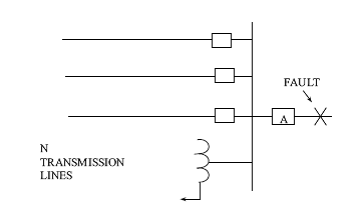
\includegraphics{f1SingleLineDiagram}
        \caption{Single Line Diagram}
        \label{fig:Single Line Diagram}
    \end{subfigure}
    
    \begin{subfigure}[b]{\textwidth}
        \centering
        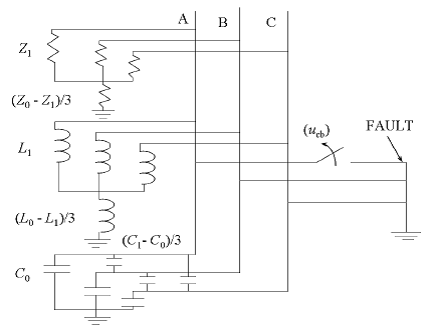
\includegraphics{f2ThreePhaseDiagram}
        \caption{Three Phase Diagram}
        \label{fig:Three Phase Diagram}
    \end{subfigure}

    \begin{subfigure}[b]{\textwidth}
        \centering
        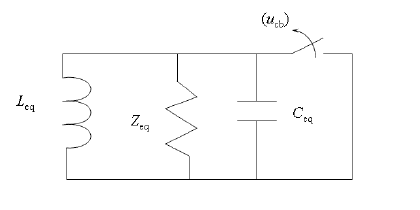
\includegraphics{f3EquivalentCircuitn}
        \caption{Equivalent Circuit}
        \label{fig:Equivalent Circuit}
    \end{subfigure}
    \caption{Circuit for Interruption of a Three-Phase-to-Ground Fault}
    \label{fig:Circuit for Interruption of a Three-Phase-to-Ground Fault}
\end{figure}

\subsubsection{Exponential (Overdamped) TRV}
The TRV across the CB contacts can be found using current injection technique as the time span is short (microseconds). The current can be represented by a ramp. The solution for the parallel RLC network shown in Figure \ref{fig:Equivalent Circuit} is given by Equation (\ref{eq:3.4}):

\begin{equation}\label{eq:3.4}
u_{cb} = u_1 \left( 1 - e^{\alpha t} \left( \cosh \beta t + \frac{\alpha}{\beta} \sinh \beta t \right) \right) kV
\end{equation}

$u_{cb}$ =  voltage across the open circuit-breaker contacts\\
$u_1 = \sqrt{2} I \omega L_{eq}, (kV)$\\
$\omega = 2 \Pi f, (rad/s)$\\
$I$ = rms value short-circuit current, (kA)\\
$\alpha = \frac{1}{2 Z_{eq} C_{eq}}$\\
$\beta =\sqrt{\alpha^2 - \frac{1}{(L_{eq} C_{eq})}}$\\
$Z_{eq}$ - equivalent impedance ($\Omega$)\\
$L_{eq}$ - equivalent inductance ($H$)\\
$C_{eq}$ - equivalent capacitance ($F$)\\

In most of the applications, the parallel resistance of the line surge impedances of the lines is such that it effectively swamps the capacitance of the circuit. Hence it is a common practice to neglect the capacitance. The solution to the simple RL circuit is given by equation (\ref{eq:3.5}):

\begin{equation}\label{eq:3.5}
u_{cb} = u_1 \left( 1 - e^{-t / \tau} \right) kV
\end{equation}
where\\
$\tau = \frac{L_{eq}}{Z_{eq}} s$

\subsubsection[Single frequency recovery voltage]{Single frequency recovery voltage\\(Oscillatory underdamped TRV)}
When the short circuit is fed by a transformer and numbers of lines remain connected to the bus, the resulting TRV is oscillatory single frequency TRV. Figure \ref{fig:Equivalent Circuit} shows the equivalent circuit with resistance removed. The circuit becomes underdamped and the response is a typical 1-cosine waveform. Equation \ref{eq:3.6} is the approximate equation for the voltage across the open circuit breaker contacts of CB.

\begin{equation}\label{eq:3.6}
u_{cb} = u_1 \left[ 1 - \cos \left( \frac{t}{\sqrt{L_{eq} C_{eq}}} \right) \right]
\end{equation}

\subsection{Traveling waves}
The transmission line can be represented as an inductive elements connected in series and capacitive elements distributed along the line in parallel. The voltage applied at one end travels as an electromagnetic wave with the speed of light. When the transmitted wave reaches discontinuity, the wave gets reflected and refracted depending on the discontinuity. The time for the wave to go out from the discontinuity and back is given by:

\begin{equation}\label{eq:3.7}
T = 6.68 l \sqrt{\mu \epsilon} ~~\mu s
\end{equation}

$l$ - distance to the first discontinuity (km)\\
$\mu$ - magnetic permeability\\
$\epsilon$ - dielectric constant

The coefficients for the new voltage waves are\\
\begin{equation}\label{eq:3.8}
\text{Reflection,~~~} K_R = \frac{Z_2 - Z_1}{Z_2 + Z_1}
\end{equation}
\begin{equation}\label{eq:3.9}
\text{Refraction,~~~} K_T = \frac{2 Z_2}{Z_2 + Z_1}
\end{equation}
$Z_1$ and $Z_2$ are the surge impedances on either side of the discontinuity.

\subsection{Short Line Fault}
The TRV across the CB contacts after the interruption of short line fault consists of the voltage generated by the supply network and of the voltage created by the line side oscillation. Due to distributed constants of the transmission line, the line side oscillations are in the form of traveling waves. The reflection of this traveling wave against the short circuit point and the open end at the breaker side cause a triangular shaped waveform.

The travel time of the electromagnetic waves in case of single line to ground fault at a distance \textquoteleft$l$\textquoteright ~from the breaker to the fault location is given by
\[
\tau_{Line} = \frac{l}{\vartheta}
\]
Where $\vartheta$ is the wave velocity that depends on the transmission line parameters. The wave reflected by the short circuit point arrives at the open end near the breaker after twice the travel time. The lattice diagram shown in figure \ref{fig:Lattice Diagram to Evaluate the Characteristics of Travelling Wave} is used to evaluate the characteristics of travelling wave for short line fault. The numerical value of the coefficients for the reflected and transmitted wave shows the amplitude multiplier for the voltage wave. Single phase circuit for short line fault with source ($X_S$) and the line reactance ( $\lambda * X_L$ ) is shown in figure \ref{fig:Single-Phase Circuit with Short-Line Fault}. The fault current is given by equation \ref{eq:3.10}.

\begin{equation}\label{eq:3.10}
I_L = \frac{u_{LG}}{\lambda \times X_L + X_s}
\end{equation}
$X_L$ - reactance of the line to the fault point per kilometer, given by $\frac{(2L_{1 \omega} + L_{0 \omega})\omega}{3}$\\
$L_1$ - positive sequence power-frequency line inductance per kilometer\\
$L_0$ - zero sequence power-frequency line inductance per kilometer\\
$u_{LG}$ - line to ground system voltage (kV)\\
$\lambda$ - distance of CB to the fault (km)\\
$I_L$ - terminal fault current (kA)

\begin{equation}\label{eq:3.11}
\frac{d u_L}{dt} = \sqrt{2} \omega I_L Z_{eff}
\end{equation}

\begin{figure}[!htbp]
    \centering
    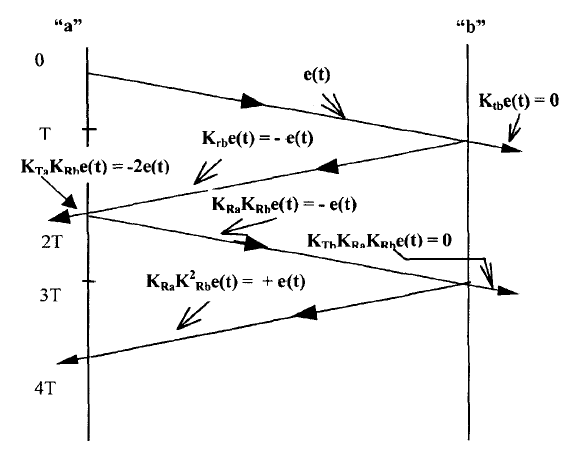
\includegraphics[width=\textwidth]{LatticeDiagramtoEvaluatetheCharacteristicsofTravellingWave}
    \caption{Lattice Diagram to Evaluate the Characteristics of Travelling Wave}
    \label{fig:Lattice Diagram to Evaluate the Characteristics of Travelling Wave}
\end{figure}

\begin{figure}
    \centering
    \begin{subfigure}[b]{0.5\textwidth}
        \centering
        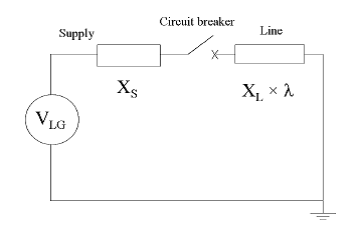
\includegraphics[width=\textwidth]{g1SinglePhaseCircuitwith}
        \caption{Single-Phase Circuit with Short-Line Fault}
        \label{fig:Single-Phase Circuit with Short-Line Fault}
    \end{subfigure}
    \\
    \begin{subfigure}[b]{0.49\textwidth}
        \centering
        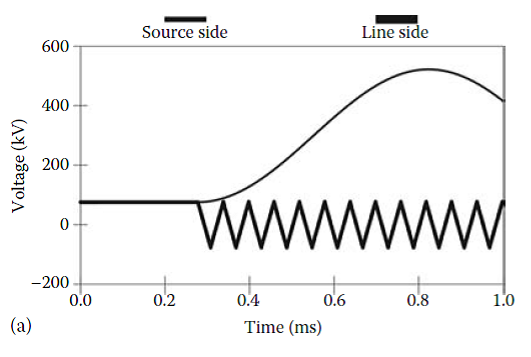
\includegraphics[width=\textwidth]{g2LineSideandSourceSideVoltages}
        \caption{Line Side and Source Side Voltages}
        \label{fig:Line Side and Source Side Voltages}
    \end{subfigure}
    \begin{subfigure}[b]{0.49\textwidth}
        \centering
        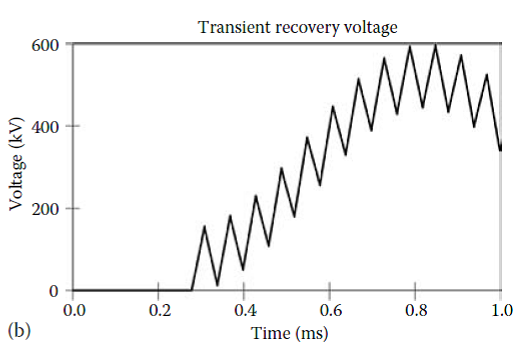
\includegraphics[width=\textwidth]{g3TransientRecoveryVoltage}
        \caption{Transient Recovery Voltage}
        \label{fig:Transient Recovery Voltage}
    \end{subfigure}
    \caption{TRV across the Breaker during Short Line Fault}
    \label{fig:TRV across the Breaker during Short Line Fault}
\end{figure}
The source side and line side TRV shapes during short line fault is shown in figure \ref{fig:TRV across the Breaker during Short Line Fault}.

\clearpage
\section{Mathematical Model}
Configuration of contacts plays a crucial role in the performance of CB. Contact resistance depends on the contact forces and the actual contact area. The contact resistance is given by

\begin{equation}
R_T = \frac{\rho}{2} \sqrt{\frac{\pi K H }{F_T}} + R_F
\end{equation}

Where:\\
$H$ - Material hardness\\
$K$ - Constant between 0.1 and 0.3\\
$\rho$  - Resistivity of contact material\\
$R_F$ - Film resistance\\
$F_T$ - Total force acting on a contact
The current get constricted at the point of contact. This constriction of current is responsible for contact resistance and the heat generated at the contacts. It is also the source of electromagnetic force that acts upon contact structure.

For a circular cluster contacts, three forces act upon: the attractive force ($F_A$), repulsive force ($F_R$) and contact spring force ($F_S$). Thus the total force ($F_T$) acting on a contact is given by 

\begin{equation}
F_T = F_S + F_R - F_A
\end{equation}

The attraction force should be greater than the repulsive force for a CB contacts. When SF\textsubscript{6} CB contacts are subjected to arcing, a sulfide coat is formed. This sulfide coat increases the contact resistance if there is no scrapping or wiping motion between the contacts. The sulfide coat gets removed by slight friction and decomposed by heat. The force of attraction exists between two opposite fingers of a circular cluster contacts when current is flowing in the same direction. This force of attraction for contact having \textquoteleft$n$\textquoteright ~ fingers and distance \textquoteleft$d$\textquoteright ~between fingers with a current of $I/n$ through each finger is given by 

\begin{equation}
F_A = 0.102 (n-1) \left( \frac{I}{n}\right)^2 \left( \frac{l}{d}\right)
\end{equation}

The attractive force pinches the moving contact fingers on the fixed contact which reduces the contact resistance as shown in Fig 3.3.1. The wiping action on the contacts get improved which helps in removing the sulfide coat \cite{hedman2009optimal}. The CB contacts should be properly designed for wiping action so that the problem of metallic fluoride deposition is minimized \cite{kezunovic2014reliable}.

\begin{figure}[!htbp]
    \centering
    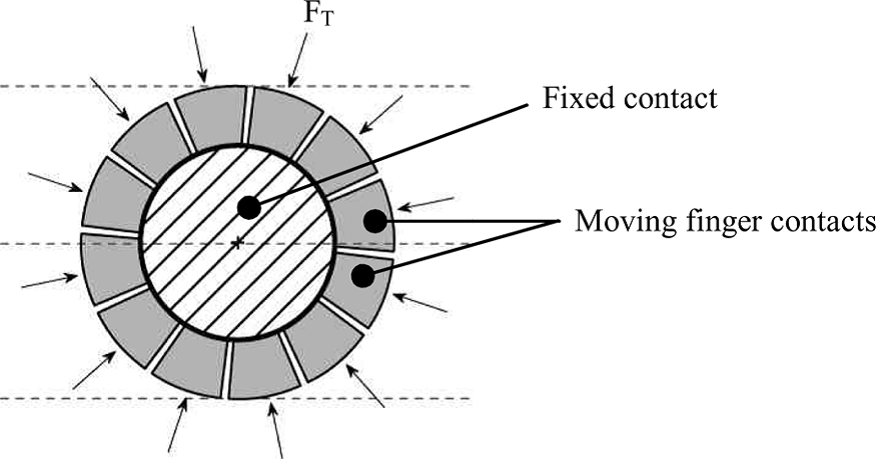
\includegraphics[width=\textwidth]{SchematicofForcesExertedontheFixed}
    \caption{Schematic of Forces Exerted on the Fixed Contact by the Moving Finger Contacts}
    \label{fig:Schematic of Forces Exerted on the Fixed Contact by the Moving Finger Contacts}
\end{figure}

CB is an electromechanical device. Hence its model is governed by mechanical and electromagnetic equations. Mechanical equation of a CB is expressed by the Newton's second law, as shown in equation \ref{eq:3.17}

\begin{equation}\label{eq:3.17}
\rho \left( \frac{\partial^2 u}{\partial t^2} \right) =  \nabla \cdot FS + F_v
\end{equation}
$F_v$ - force per unit volume of deformed mass (N)\\
$\rho$ - mass density ($kg/m^3$)\\ 
$S$ - second order Piola-Kirchhoff stress\\
$F$ - deformation gradient\\
$U$ - mechanical displacement (m) 

Electromagnetic equations of CB are expressed by (\ref{eq:3.18})-(\ref{eq:3.22})

\begin{equation}\label{eq:3.18}
J = \sigma E + J_e
\end{equation}
\begin{equation}
E = - \nabla V
\end{equation}
\begin{equation}
\nabla \cdot J = Q_j
\end{equation}
\begin{equation}
\nabla \times (\mu \nabla \times A_z) = J
\end{equation}
\begin{equation} \label{eq:3.22}
F = J \times B
\end{equation}

$\sigma$ - electrical conductivity $(S/m)$\\
$J_e$ - applied current density $(A/m^2)$\\ 
$J$ - current density $(A/m^2)$\\ 
$V$ - voltage (V) \\
$E$ - electric field $(V/m)$ \\
$Q_j$ - charge per unit volume $(C/m^3)$\\
$\mu$ - average permeability\\
$A_z$ - magnetic vector potential\\
$B$ - magnetic field in Tesla \\
$F$ - magnetic force of the Lorentz law (N)

Passage of electricity produces heat, and this heat affects the resistance and electrical and mechanical properties of CB. 

\subsection{Contact resistance measurement method}
Standard Timing test is performed on breaker followed by static contact resistance measurement. Figure \ref{fig:Schematic Diagram of Static Contact Resistance Measurement} shows the arrangement for static contact resistance measurement. The value of test current should be as per the manufactures specifications. IEC and ANSI recommend 50 A and 100 A respectively. Breaker is kept in closed position. 100 A DC current is passed through the contacts. Voltage drop is measured and contact resistance is calculated.

\begin{figure}[!htbp]
    \centering
    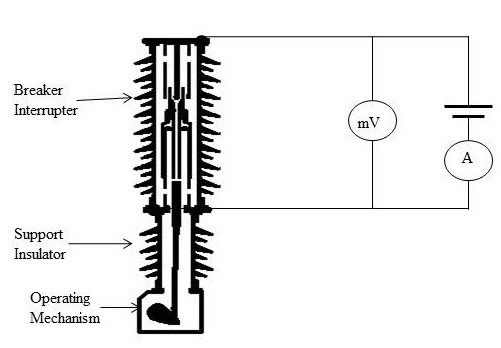
\includegraphics[width=\textwidth]{SchematicDiagramofStaticContactResistanceMeasurement}
    \caption{Schematic Diagram of Static Contact Resistance Measurement}
    \label{fig:Schematic Diagram of Static Contact Resistance Measurement}
\end{figure}

\begin{figure}[!htbp]
    \centering
    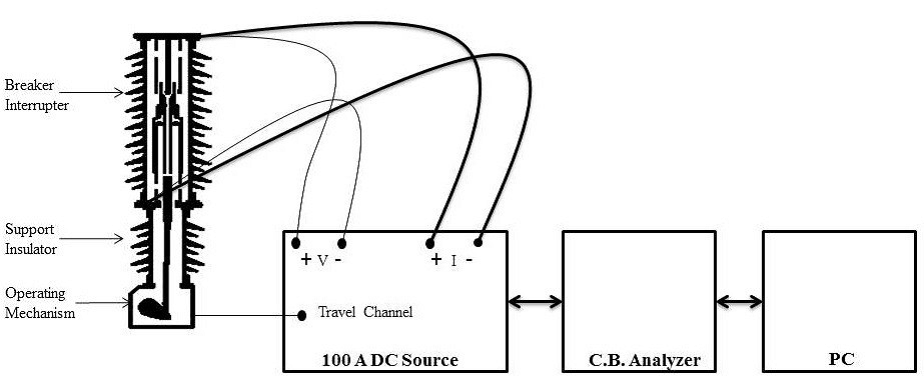
\includegraphics[width=\textwidth]{SchematicDiagramofDCRM}
    \caption{Schematic Diagram of DCRM}
    \label{fig:Schematic Diagram of DCRM}
\end{figure}

The schematic diagram of DCRM is shown in figure \ref{fig:Schematic Diagram of DCRM}. The close-trip command is given to CB. 100A DC current is injected, and the CB is operated at rated speed. Depending on the breaker technology, linear or rotary contact travel transducer is used for recording contact movement. The instantaneous value of resistance is measured along with contact travel. The test kit of Scope Company with Hisac Ultima test manager software for analysis is used. Measuring system with a sampling frequency of 10 kHz and 100 $\mu s$ resolution is used to record the resistance with precision as well as to record the transfer of current from arcing contact to the main contact and vice-versa. A time delay of 300 ms is kept between close-trip operations. The test set up is connected to a portable computer for calculation of instantaneous contact resistance, data analysis and interpretation using the software. The variations in the resistance over time are recorded as a finger print for the breaker contacts. This recorded signature can be used as a benchmark for comparison of the future measurement record of the same breaker. The DCRM signature provides information on the breaker contacts and the operating mechanism. Measuring system and test set up is shown in Figure \ref{fig:Test set up for DCR Measurement}.

\begin{figure}
    \centering
    \begin{subfigure}[b]{0.49\textwidth}
        \centering
        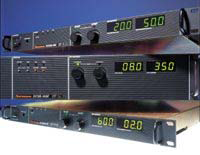
\includegraphics[width=\textwidth]{h1Stablecurrentsource}
        \caption{Stable Current Source}
        \label{fig:Stable current source}
    \end{subfigure}
    \\
    \begin{subfigure}[b]{0.49\textwidth}
        \centering
        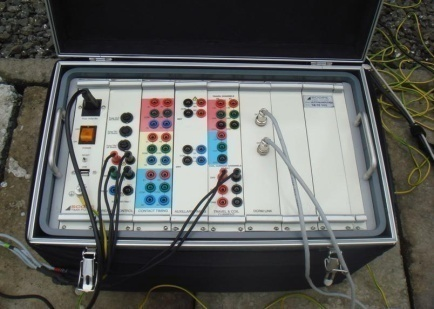
\includegraphics[width=\textwidth, height = 5cm]{h2Dataacquisitionsystem}
        \caption{Data Acquisition System}
        \label{fig:Data acquisition system}
    \end{subfigure}
    \begin{subfigure}[b]{0.49\textwidth}
        \centering
        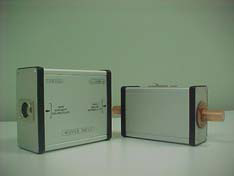
\includegraphics[width=\textwidth, height = 5cm]{h3VoltageandCurrentsensors}
        \caption{Voltage and Current Sensors}
        \label{fig:Voltage and Current sensors}
    \end{subfigure}
    \\
    \begin{subfigure}[b]{0.49\textwidth}
        \centering
        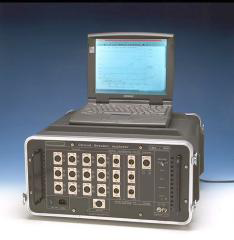
\includegraphics[width=\textwidth]{h4Testmanagersoftware}
        \caption{Test Manager Software}
        \label{fig:Test manager software}
    \end{subfigure}
    \caption{Test Set Up for DCR Measurement}
    \label{fig:Test set up for DCR Measurement}
\end{figure}

\subsection{DCRM signature analysis}
Figure \ref{fig:Measurement Details from DCRM Signature} shows the measurement details from DCRM signature. DCRM may be called as an ECG of the circuit breaker. The analysis software provided with a test kit can be used for analysis. However, analysis of signature needs the knowledge of CB design, interrupter design, operating mechanism and also expertise to detect the problem. Every CB has a different shape of DCRM signature which mainly depends on contact design, type of operating mechanism, contact wipe, contact speed, \textit{etc}. The deviations in the signature can be found by superimposing earlier signature. Parameters such as length of arcing contact, erosion of contacts, mechanical problem, contact travel and speed, healthiness of mechanism, \textit{etc}. can be obtained from the signature. An enlarged view of DCRM signature in the tripping zone is shown in figure \ref{fig:Enlarged View of Tripping Portion of DCRM Signature}.

\begin{figure}[!htbp]
\centering
\begin{minipage}{\textwidth}
\centering
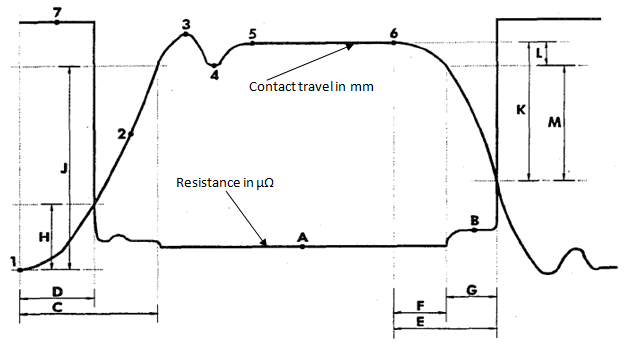
\includegraphics[width=\textwidth]{MeasurementDetailsfromDCRMSignature}
\caption{Measurement Details from DCRM Signature}
\label{fig:Measurement Details from DCRM Signature}
\begin{flushleft}
\footnotesize A: main contact resistance\\
B: arcing contact resistance\\
C: time for main contacts to make\\
D: time for arcing contacts to make\\
E: time for arcing contacts to break\\
F: time for main contacts to break\\
G: time arcing contact made\\
H: distance for arcing contacts to make\\
J: distance for main contacts to make\\
K: distance for arcing contacts to break\\
L: distance for main contacts to break (wipe of main contact)\\
M: distance arcing contacts made (wipe of arcing contact)\\
\end{flushleft}
\end{minipage}
\end{figure}

\begin{figure}[!htbp]
    \centering
    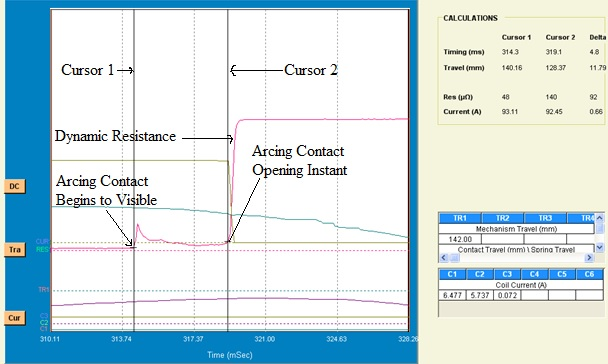
\includegraphics[width=\textwidth]{EnlargedViewofTrippingPortionofDCRMSignature}
    \caption{Enlarged View of Tripping Portion of DCRM Signature}
    \label{fig:Enlarged View of Tripping Portion of DCRM Signature}
\end{figure}

\subsection{Case studies}
POWERGRID and many utility companies in India are using DCRM test for condition assessment of CBs. Case studies from the field are discussed in this section which signifies the use of DCRM signature in detecting the problems at an early stage in CBs.

\subsubsection*{Case no. 1}
Contact bouncing~ for longer duration~ in no load closing characteristics~ at manufacturer works (Figures \ref{fig:Contact Bouncing after Closing Cycle on 400 kV SF6 Circuit Breaker} to \ref{fig:DCRM Signature Showing Fluctuations in Resistance Curve of B Phase Front Side Interrupter}) was seen for a 400 kV SF\textsubscript{6} CB during closing operation. The bouncing was noticed after the completion of mechanical travel. Problem was analyzed in the following steps:

\begin{enumerate}
\item The external connections were verified and were found normal. The connections of the test leads connecting main contacts to analyzer were also checked and found correct. The test was repeated with a different analyzer to rule out the electrical signaling fault. But the same problem persisted. It was then confirmed that the problem is within the interrupter assembly

\item Static contact resistance was measured and found to be very high 120 to 160 k$\Omega$

\item The bouncing in the no load closing characteristics is verified by conducting the DCRM test of a B-phase front side interrupter

\item Lot of fluctuations in the current and resistance curve in the no action zone was observed in the DCRM signature

\item Abnormal DCRM signature for the rear side of the same pole was obtained even though no abnormal contact bouncing was seen in no load closing operation

\item The investigations in subassemblies were done in steps and the cause of the problem was detected in moving contact assembly. The puffer cylinder and cylinder support joint was found loose. During assembly of the interrupter, tightening torque was not applied
\end{enumerate}

\begin{figure}[!htbp]
    \centering
    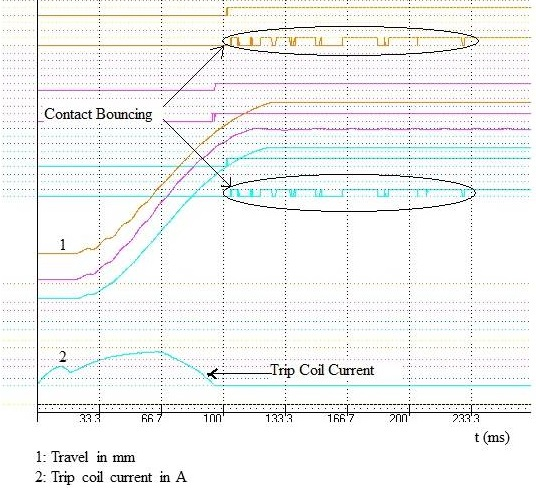
\includegraphics[width=\textwidth]{ContactBouncingafterClosingCycle}
    \caption{Contact Bouncing after Closing Cycle on 400 kV SF\textsubscript{6} Circuit Breaker}
    \label{fig:Contact Bouncing after Closing Cycle on 400 kV SF6 Circuit Breaker}
\end{figure}

\begin{figure}[!htbp]
    \centering
    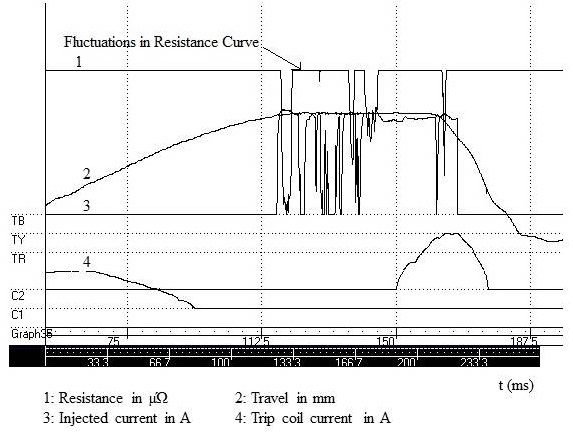
\includegraphics[width=\textwidth]{DCRMSignatureShowingFluctuationsinResistance}
    \caption{DCRM Signature Showing Fluctuations in Resistance Curve of B Phase Front Side Interrupter}
    \label{fig:DCRM Signature Showing Fluctuations in Resistance Curve of B Phase Front Side Interrupter}
\end{figure}

\subsubsection*{Case no. 2}
For a 245 kV SF\textsubscript{6} CB, contact mismatch was observed in the opening operation. The mismatch was not getting adjusted with spring and coil adjustments. The speed time graph was analyzed and following points were noticed:

\begin{enumerate}
\item For R and Y poles, abnormal contact bouncing for more than 5 milliseconds was observed in closing operation

\item As compared to B pole, the wipe was less for R and Y pole in opening operation
\end{enumerate}

The DCRM signatures were obtained for all three phases. The signatures were analyzed for closing and tripping. As seen in the figures \ref{fig:Enlarged View of R-Pole DCRM in Closing Part} and \ref{fig:R-Pole DCRM in Tripping Zone}, abnormality in travel curve and current, as well as resistance, was observed. DCRM of R-pole during tripping can be seen in figure \ref{fig:Y-Pole DCRM in Tripping Zone}. The CB was opened. It was observed that 145 kV arcing contact was fitted instead of 245 kV arcing contact during assembly as seen in figure \ref{fig:Wrong Assembly of Arcing Contact}. DCRM signatures were normal after fitting proper arcing contact.

\begin{figure}[!htbp]
    \centering
    \includegraphics[width=\textwidth]{EnlargedViewofRPoleDCRM}
    \caption{Enlarged View of R-Pole DCRM in Closing Part}
    \label{fig:Enlarged View of R-Pole DCRM in Closing Part}
\end{figure}

\begin{figure}[!htbp]
    \centering
    \includegraphics[height=4in]{RPoleDCRMinTrippingZone}
    \caption{R-Pole DCRM in Tripping Zone}
    \label{fig:R-Pole DCRM in Tripping Zone}
\end{figure}

\begin{figure}[!htbp]
    \centering
    \includegraphics[height=4in]{YPoleDCRMinTrippingZone}
    \caption{Y-Pole DCRM in Tripping Zone}
    \label{fig:Y-Pole DCRM in Tripping Zone}
\end{figure}

\begin{figure}[!htbp]
    \centering
    \includegraphics[width=\textwidth]{WrongAssemblyofArcingContact}
    \caption{Wrong Assembly of Arcing Contact}
    \label{fig:Wrong Assembly of Arcing Contact}
\end{figure}

\subsubsection*{Case no. 3}
The no load opening graph of a 245 kV SF\textsubscript{6} CB during closing was normal as observed in figure \ref{fig:Closing Graph of 245 kV SF6 Circuit Breaker}. But contact bouncing and current breaking in the closing part of the DCRM (Figure \ref{fig:Complete DCRM Signature of 245 kV SF6 Circuit Breaker}) was seen. The DCRM in the tripping portion is shown in figure \ref{fig:DCRM of 245 kV SF6 Circuit Breaker in Tripping Zone}. The closing operation was repeated, and bouncing was seen in the closing graph (Figure \ref{fig:Contact Bouncing in Closing Graph of 245 kV SF6 Circuit Breaker}). The interrupter was opened, and it was observed that moving arcing contact was become loose. The required tightening torque was not applied during assembly. In consequent mechanical operations, it started becoming more and more loose. After rectification of the problem, the normal signature was obtained.

\begin{figure}[!htbp]
    \centering
    \includegraphics[height=4in]{ClosingGraphof245kV}
    \caption{Closing Graph of 245 kV SF\textsubscript{6} Circuit Breaker}
    \label{fig:Closing Graph of 245 kV SF6 Circuit Breaker}
\end{figure}

\begin{figure}[!htbp]
    \centering
    \includegraphics[height=4in]{CompleteDCRMSignatureof245}
    \caption{Complete DCRM Signature of 245 kV SF\textsubscript{6} Circuit Breaker}
    \label{fig:Complete DCRM Signature of 245 kV SF6 Circuit Breaker}
\end{figure}

\begin{figure}[!htbp]
    \centering
    \includegraphics[height=4in]{DCRMof245kVSF6}
    \caption{DCRM of 245 kV SF\textsubscript{6} Circuit Breaker in Tripping Zone }
    \label{fig:DCRM of 245 kV SF6 Circuit Breaker in Tripping Zone}
\end{figure}

\begin{figure}[!htbp]
    \centering
    \includegraphics[height=4in]{ContactBouncinginClosingGraph}
    \caption{Contact Bouncing in Closing Graph of 245 kV SF\textsubscript{6} Circuit Breaker}
    \label{fig:Contact Bouncing in Closing Graph of 245 kV SF6 Circuit Breaker}
\end{figure}
\clearpage

\subsubsection*{Case no. 4}
Contact resistance measurement of a 220 kV SF\textsubscript{6} CB used for switching 220/33 kV, 50 MVA transformer in 400 kV substation, Waluj, Aurangabad showed a high value of resistance of the order of 200 kΩ for R-pole. The measurement test was repeated, and it was showing higher values. After repeated tests, the result was found to be higher value for resistance. DCRM test was conducted. A lot of fluctuations were observed in the resistance in no action zone of the DCRM signature as shown in figure \ref{fig:Abnormal Variations in Resistance in no Action Zone of DCRM Signature for 220 kV Circuit Breaker}. DCRM test was repeated again after confirming the connections. No change was observed in the signature. It was decided to open the R-pole. It was observed that the ring connecting the PTFE nozzle of the main contact became loose. Scratch marks were also found as seen in figure \ref{fig:Loose Ring Connecting PTFE Nozzle of Main Contact}. The signature was normal after attending the problem.

\begin{figure}[!htbp]
    \centering
    \includegraphics[width=\textwidth]{AbnormalVariationsinResistanceinno}
    \caption{Abnormal Variations in Resistance in no Action Zone of DCRM Signature for 220 kV Circuit Breaker}
    \label{fig:Abnormal Variations in Resistance in no Action Zone of DCRM Signature for 220 kV Circuit Breaker}
\end{figure}

\begin{figure}[!htbp]
    \centering
    \includegraphics[height = 4in]{LooseRingConnectingPTFE}
    \caption{Loose Ring Connecting PTFE Nozzle of Main Contact}
    \label{fig:Loose Ring Connecting PTFE Nozzle of Main Contact}
\end{figure}

\subsubsection*{Case no. 5}
Abnormal peak in the DCRM signature in the close zone portion of a 400 kV CB was seen in after three years of installation. The static contact resistance was found be 150 $\mu \Omega$. The CB was opened for contact inspection. Following observations were made.

\begin{enumerate}
\item This breaker has seen more fault operations and high current making and breaking operations

\item Due to arcing between contacts in SF\textsubscript{6} gas environment metal fluorides and metal sulfates were formed inside arcing chamber which increased the resistance to considerable value

\item Because of high temperature attained during arcing, finger contacts of moving arc contact got expanded and contact burning at both side caused abnormal DCRM

\item Because of early detection of faulty internal condition through DCRM testing, major failure is avoided
\end{enumerate}

Figures \ref{fig:Problematic DCRM Signature} to \ref{fig:Deposition of Sulfide Powder on Contact Assembly} indicates the signature and internal contact conditions of the CB.

\begin{figure}[!htbp]
    \centering
    \includegraphics[width=0.8\textwidth]{ProblematicDCRMSignature}
    \caption{Problematic DCRM Signature}
    \label{fig:Problematic DCRM Signature}
\end{figure}

\begin{figure}[!htbp]
    \centering
    \includegraphics[width=0.8\textwidth]{IncreaseinResistanceinCloseZone}
    \caption{Increase in Resistance in Close Zone}
    \label{fig:Increase in Resistance in Close Zone}
\end{figure}
%*************************************************************
%\begin{figure}
%    \centering
%    \begin{subfigure}[b]{0.3\textwidth}
%        \centering
%        \includegraphics[width=\textwidth]{i1Movingcontactassemblyinside}
%        \caption{Moving contact assembly inside porcelain}
%        \label{fig:Moving contact assembly inside porcelain}
%    \end{subfigure}
%
%    \begin{subfigure}[b]{0.3\textwidth}
%        \centering
%        \includegraphics[width=\textwidth]{i2Stationarycontactassembly}
%        \caption{Stationary contact assembly}
%        \label{fig:Stationary contact assembly}
%    \end{subfigure}
%    \\
%    \begin{subfigure}[b]{0.3\textwidth}
%        \centering
%        \includegraphics[width=\textwidth]{i3Fixedandmovingcontacts}
%        \caption{Fixed and moving contacts in engaged condition after removal from porcelain}
%        \label{fig:Fixed and moving contacts in engaged condition after removal from porcelain}
%    \end{subfigure}
%    
%    \begin{subfigure}[b]{0.3\textwidth}
%        \centering
%        \includegraphics[width=\textwidth]{i4Movingcontactassembly}
%        \caption{Moving contact assembly after Teflon removal}
%        \label{fig:Moving contact assembly after Teflon removal}
%    \end{subfigure}
%    \\
%    \begin{subfigure}[b]{0.3\textwidth}
%        \centering
%        \includegraphics[width=\textwidth]{i5Fixedcontactassembly}
%        \caption{Fixed contact assembly}
%        \label{fig:Fixed contact assembly}
%    \end{subfigure}
%    
%    \caption{Fix and Moving Contact Assembly}
%    \label{fig:Fix and Moving Contact Assembly}
%\end{figure}
%***********************************************************************************
\begin{figure}
    \centering
    \begin{subfigure}[b]{0.3\textwidth}
        \centering
        \includegraphics[width=\textwidth, height=6cm]{i1Movingcontactassemblyinside}
        \caption{Moving contact assembly inside porcelain}
        \label{fig:Moving contact assembly inside porcelain}
    \end{subfigure}
    \begin{subfigure}[b]{0.3\textwidth}
        \centering
        \includegraphics[width=\textwidth, height=6cm]{i2Stationarycontactassembly}
        \caption{Stationary contact assembly}
        \label{fig:Stationary contact assembly}
    \end{subfigure}
    \begin{subfigure}[b]{0.3\textwidth}
        \centering
        \includegraphics[width=\textwidth, height=6cm]{imInside}
        \vspace{0.9cm}
    \end{subfigure}
    \\
    \begin{subfigure}[b]{0.3\textwidth}
        \centering
        \includegraphics[width=\textwidth, height=5cm]{i3Fixedandmovingcontacts}
        \caption{Fixed and moving contacts in engaged condition after removal from porcelainn}
        \label{fig:Fixed and moving contacts in engaged condition after removal from porcelain}
    \end{subfigure}
    \begin{subfigure}[b]{0.3\textwidth}
        \centering
        \includegraphics[width=\textwidth, height=5cm]{i4Movingcontactassembly}
        \caption{Moving contact assembly after Teflon removal}
        \label{fig:Moving contact assembly after Teflon removal}
        \vspace{0.7cm}
    \end{subfigure}
    \begin{subfigure}[b]{0.3\textwidth}
        \centering
        \includegraphics[width=\textwidth, height=5cm]{i5Fixedcontactassembly}
        \caption{Fixed contact assembly}
        \label{fig:Fixed contact assembly}
        \vspace{1.4cm}
    \end{subfigure}
    \caption{Fix and Moving Contact Assembly}
    \label{fig:Fix and Moving Contact Assembly}
\end{figure}

%***********************************************************************************
\begin{figure}
    \centering
    \begin{subfigure}[b]{0.49\textwidth}
        \centering
        \includegraphics[width=\textwidth, height=7cm]{j1PufferCylinderSlidingContacts}
        \caption{Puffer Cylinder Sliding Contacts}
        \label{fig:Puffer Cylinder Sliding Contacts}
    \end{subfigure}
    \begin{subfigure}[b]{0.49\textwidth}
        \centering
        \includegraphics[width=\textwidth, height=7cm]{j2MainMovingContact}
        \caption{Main Moving Contact}
        \label{fig:Main Moving Contact}
    \end{subfigure}
    \\
    \begin{subfigure}[b]{0.49\textwidth}
        \centering
        \includegraphics[width=\textwidth, height=6cm]{j3MovingArcContactSideofNozzle}
        \caption{Moving Arc Contact Side of Nozzle}
        \label{fig:Moving Arc Contact Side of Nozzle}
    \end{subfigure}
    \begin{subfigure}[b]{0.49\textwidth}
        \centering
        \includegraphics[width=\textwidth, height=6cm]{j4StationaryContactSideofNozzle}
        \caption{Stationary Contact Side of Nozzle}
        \label{fig:Stationary Contact Side of Nozzle}
    \end{subfigure}
    
    \caption{Deposition of Sulfide Powder on Contact Assembly}
    \label{fig:Deposition of Sulfide Powder on Contact Assembly}
\end{figure}

\clearpage
\section[New Algorithm for Contact Condition Detection of SF\textsubscript{6} CB]{New Algorithm for Contact Condition \\Detection of SF\textsubscript{6} CB}

Tests were conducted on 400 kV and 245 kV SF\textsubscript{6} CBs at circuit breaker manufacturing industry, 400 kV substation Waluj, Aurangabad and 765 kV substation at Thapti Tanda Aurangabad. Timing measurement, SCRM as well as DCRM tests were conducted. Data of DCRM for healthy breakers as well as breakers with problems in condition of contact was collected from the largest utility company PGCIL as well as MSETCL. Figure \ref{fig:DCRM Signature Showing the Parameters used in Algorithm} shows the DCRM signature in the tripping portion along with the parameters.

\begin{figure}[!htbp]
    \centering
    \includegraphics[width=\textwidth]{DCRMSignatureShowingtheParametersusedinAlgorithm}
    \caption{DCRM Signature Showing the Parameters used in Algorithm}
    \label{fig:DCRM Signature Showing the Parameters used in Algorithm}
\end{figure}

Following parameters are used for developing contact wear algorithm:

$T_m$ - time at the position when main contact disengages (ms)\\
$T_a$ - time at the position when arc contact disengages (ms)\\
$R_{aimax}$ - arc contact resistance at the point of main contact disengagement ($\mu \Omega$)\\
$A_m$ - area below the main contact resistance zone ($\mu \Omega \times$ms)\\
$A_a$ - area under the arc contact zone ($\mu \Omega \times$ms)\\
$R_m$ - average contact resistance in the main contact region ($\mu \Omega$)\\
$R_a$ - average contact resistance in the arc contact region ($\mu \Omega$)

Deviations in the above parameters from the healthy DCRM signature will be used for developing the contact wear algorithm. Number of DCRM signatures was analyzed and following observations are made. 

\subsubsection*{Fixed arc contact tip wear}
Over the times due to arcing and heat, length of fixed arc contact reduces. Shortening of fix arc contact will be reflected at the end of the resistance curve during tripping portion. Position at which the arc contact disengages finally will shift to left than normal curve. Average arc contact resistance will increase, but the area below the DCRM curve in arc contact zone will decrease due to earlier disengagement of arc contact. Since main contact condition is sound, the point at which main contact disengages will remain same so also the area below the main contact resistance zone. In this case, the motion will start earlier than in previous measurement indicating wearing of contact.$\Delta T_m = 0, \Delta T_a < 0, \Delta A_a < 0, \Delta R_{aimax} = 0$ and $\Delta A_m = 0$. Arcing contact wipe will decrease.

\subsubsection*{Wearing of moving arc contact}
Excessive heat and arcing also damage the fingers of arc contact. Damage to fingers will increase the initial resistance of the arc contact at the point of disengagement of the main contact. As the fix arc contact is assumed to be sound, the position of arc contact disengagement will remain same. The area under the arc contact zone will increase. This will lead to the conditions $\Delta T_m = 0, \Delta T_a = 0, \Delta A_a > 0, \Delta R_{aimax} > 0$ and $\Delta A_m = 0$. Erosion of the moving arc contact will increase the resistance in the arc contact zone.

\subsubsection*{Main contact erosion}
If the force of the fingers of the main contact is not proper or the contacts are not aligned properly, or the tightening torque is not applied then the main contact may erode. This will not change the position of arc contact disengagement but will certainly change the point of main contact disengagement. This will slightly increase the area below the arc contact zone. Variations in the no action zone of the DCRM will be seen which will increase the average main contact resistance. Increase in resistance during static contact resistance measurement can also be observed. The condition will be $ \Delta T_m < 0, \Delta A_a > 0, \Delta T_a = 0, \Delta R_{aimax} = 0, \Delta A_m > 0$.

\subsubsection*{Arc contact (fixed and moving) and main contact erosion}
Erosion of fixed arc contact and main contact will change both the position of main and arc contact displacement resulting in reduction in area below the arc contact region and increasing the arc contact resistance at the disengagement of main contact resistance position at the same time variations in the close portion of the DCRM is also observed increasing the area below the main contact resistance zone. Arcing contact wipe will be reduced leading to a condition of $ \Delta T_m < 0, \Delta T_a < 0, \Delta A_a < 0, \Delta R_{aimax} > 0, \Delta A_m >0$.

\subsubsection*{Fix and Moving arc contact erosion}
Excessive arcing and heating may shorten the fixed arc contact at the same time melting at the fingers of moving contact may happen over the years due to switching of short circuit currents or frequent capacitor switching. This condition can be identified as $\Delta A_a < 0, \Delta T_a < 0, \Delta T_m = 0, \Delta R_{aimax} > 0$ and $ \Delta A_m = 0 $.

Based on the analysis of field DCRM, an algorithm is proposed for detecting the contact wear. Deviations in the DCRM signature from normal values are the input to the algorithm. Five parameters, deviation in the main contact cut off time ($\Delta T_a$), arcing contact cut off time ($\Delta T_a$), area below the curve in arc contact zone ($\Delta A_a$), arc contact resistance at the point of main contact disengagement ($\Delta R_{aimax}$) and the area below the curve in main contact zone ($\Delta A_m$) are used. Following cases of contact erosion is identified:
\clearpage

\begin{description}
\item[Problem 1:] Main contact erosion
\item[Problem 2:] Fix arcing contact erosion
\item[Problem 3:] Wearing of arcing contact fingers
\item[Problem 4:] Fix and Moving arcing contact erosion
\item[Problem 5:] Arcing contact (Fix and Moving) and main contact erosion
\end{description}

%************* Three Page Figure*****************************************
\begin{figure}[!ht]
\centering
    \includegraphics[width=\textwidth, height=9.69in ]{FlowChartofProposedAlgorithm1}
\end{figure}
\begin{figure}[!ht]
\centering
    \includegraphics[width=\textwidth, height=9.69in]{FlowChartofProposedAlgorithm2}
\end{figure}
\clearpage
\begin{figure}[H]
    \centering
    \begin{tabular}{| c | l |}
	\hline
	\textbf{Problem} & \multicolumn{1}{|c|}{\textbf{Description}} \\ \hline
	1					& Main contact erosion \\ \hline
	2					& Fix arcing contact erosion \\ \hline
	3					& Wearing of arcing contact fingers \\ \hline
	4					& Fix and moving arc contact erosion \\ \hline
	5					& Arc contact (Fix and moving) and main contact erosion\\ \hline
	\end{tabular}
    \caption{Flow Chart of Proposed Algorithm}
    \label{fig:Flow Chart of Proposed Algorithm}
\end{figure}

Figure \ref{fig:Flow Chart of Proposed Algorithm} shows the flow chart for the proposed algorithm. A program is developed in Java which depicts the health of CB.
%***************************************************************************

%\begin{tabular}{| >{\arraybackslash}m{1.9in} |>{\centering\arraybackslash}m{0.6in} |>{\arraybackslash}m{2.75in} |}



\chapter{PERFORMANCE ANALYSIS}
%Performance analysis
Simulation of an IEEE network is carried out in EMTP-RV for determining the short circuit capability of CB under different fault conditions. The results are obtained for the following fault conditions.
\begin{enumerate}
\item Interruption of three phase to ground fault at the terminal of substation for switching multiple lines connected to the substation

\item Interruption of three phase to ground fault at the terminal of substation for the case of transformer switching

\item Interruption of single phase to ground short line fault and modeling the line as constant parameter and frequency dependent and comparing the results for the two

\item Interruption of three phase to ground fault at the terminal of substation with arc model
\end{enumerate}

\section{Computational Analysis}

\subsection{Simulation results for case-I}
Simulation is carried out for interruption of three phase to ground fault at the terminal of the substation for switching multiple lines connected to the substation. Stray capacitance of substation equipments is considered for simulation. Current in the steady state under fault condition is measured which is 17.2 kA. For a breaker of 30 kA short circuit interruption capabilities, the standard TRV for T60 duty is modeled by four parameter method. The rating of TRV for T60 duty is obtained from the application guide shown in the Table \ref{table:: TRV Rating for 30 kA Short Circuit Current Interruption}.The simulation time step of 1$\mu s$ is used. The standard TRV and the TRV across the breaker is shown in the waveforms from figure \ref{Fig:4.1.1} to figure \ref{Fig:4.1.3}. The TRV waveform is exponential as seen in figure \ref{Fig:4.1.3}. In this case when the CB is used to switch the multiple lines, CB has inductance and capacitance on source side as well as on the load side which results in double frequency recovery voltage.

\subsection{Simulation results for case-II}
Simulation is carried out for interruption of three phase to ground fault at the terminal of a substation for the case of transformer switching. The simulation time step of 1$\mu s$ is used. As seen in the waveforms from figure \ref{Fig:4.1.4} to figure \ref{Fig:4.1.7}, the TRV is oscillatory since the fault is limited by the transformer only. The electric energy is redistributed among equivalent single capacitive and single inductive elements. In this case since the CB is used for transformer switching with no transmission lines, the circuit becomes underdamped and the resulting TRV is a typical one minus cosine waveform.

\subsection{Simulation results for case-III}
Simulation is carried out for interruption of single phase to ground short line fault at various fault distance from 1.2 km to 6.2 km for a 16 km transmission line. The lines are first modeled in constant parameter mode, and TRV is recorded. Then the lines are modeled in frequency dependent mode, and TRV is recorded. TRV in both models is compared. Time step of 0.1 $\mu s$ is used. Obtained waveforms are shown from figure \ref{Fig:4.1.8} to figure \ref{Fig:4.1.15}. The reflections of the travelling waves against short circuit point and the open end at the breaker side causes a triangular shaped waveform. The increase in line length increases the line impedance and the amplitude of the triangular shaped line side oscillation which decreases the fault current; hence $di/dt$ becomes lower. The characteristic impedance $Z_{line}$ depends on the line parameters and remains constant. Hence the RRRV decreases with increase in line length and vice-versa.

\subsection{Simulation results for arc interruption}
Simulation is carried out for interruption of three phase to ground fault at the terminal of a substation for switching multiple lines connected to the substation as well as transformer switching. Black Box Cassie-Mayer model is used for arc interruption studies. Time step of 0.1 $\mu s$ is used. The waveforms are shown in figure \ref{Fig:4.1.16} to figure \ref{Fig:4.1.17}.

\begin{sidewaystable}[!htbp]
\renewcommand{\arraystretch}{1.3}
\caption{TRV Rating for 30 kA Short Circuit Current Interruption}
\label{table:: TRV Rating for 30 kA Short Circuit Current Interruption}
\centering
\small
\begin{tabular}{ | >{\centering\arraybackslash}m{0.7in} | >{\centering\arraybackslash}m{0.7in} | >{\centering\arraybackslash}m{0.7in} | >{\centering\arraybackslash}m{0.7in} | >{\centering\arraybackslash}m{0.7in} | >{\centering\arraybackslash}m{0.5in} | >{\centering\arraybackslash}m{0.7in} | >{\centering\arraybackslash}m{0.5in} | >{\centering\arraybackslash}m{0.5in} | >{\centering\arraybackslash}m{0.6in} | >{\centering\arraybackslash}m{0.5in} | >{\centering\arraybackslash}m{0.7in} | } \hline
Rated voltage & Test duty & First pole to clear factor & Amplitude factor & First reference voltage & Time & TRV Peak value & Time & Time delay & Voltage & Time & Rate of rise \\ \hline
U1& & kpp & kaf & u1 & t1 	& uc & t2 or t3 & Td   & U' & t'   & u1/t1 \\
kV& & 	  & 	& kV &$\mu$s& uc & $\mu$s	&$\mu$s& kV &$\mu$s& uc/t3 \\
	& & & & & & & & & & 									& kV/$\mu$s \\ \hline

\multirow{5}{*}{145} &T100&1.3& 1.40& 115& 58& 215& 232& 2(16)& 58& 31(45)& 2 \\ \cline{2-12}
&\textbf{T60}& \textbf{1.3}& \textbf{1.50}& \textbf{115}& \textbf{38}& \textbf{231}& \textbf{228}& \textbf{2-12}& \textbf{58}& \textbf{21-31}& \textbf{3} \\ \cline{2-12}
&T30& 1.3& 1.54& -& -& 237& 47& 7& 79& 23& 5 \\ \cline{2-12}
&T10& 1.5& 0.9$\times$1.7& -& -& 272& 39& 6& 91& 19& 7 \\ \cline{2-12}
&Op1-Op2& 2& 1.25& 178& 178& 296& 232-464& 2-12& 89& 60-70& 1.54 \\ \hline
\end{tabular}
\end{sidewaystable}

\begin{sidewaysfigure}
   \centering 
   \includegraphics[width=\textwidth]{1trvcb2p2411} 
   \caption{TRV Waveform of the Three Phases for Multiple Line Switching at Terminal of Substation for Three Phase to Ground Fault}
   \label{Fig:4.1.1} 
\end{sidewaysfigure}

%***********************************************************************************************

\begin{sidewaysfigure}
   \centering 
   \includegraphics[width=\textwidth]{2trvawithstdcbp2412} 
   \caption{TRV Waveform of Phase A with Standard TRV and Delay Line for Multiple Line Switching at Terminal of Substation for Three Phase to Ground Fault}
   \label{Fig:4.1.2} 
\end{sidewaysfigure}

%***********************************************************************************************

\begin{sidewaysfigure}
   \centering 
   \includegraphics[width=\textwidth]{3trvawithstdenlargedcbp2413} 
   \caption{Standard TRV Envelope and Phase A TRV for Multiple Line Switching at Terminal of Substation for Three Phase to Ground Fault}
   \label{Fig:4.1.3} 
\end{sidewaysfigure}

%***********************************************************************************************

\begin{sidewaysfigure}
   \centering 
   \includegraphics[width=\textwidth]{4completetrvcb1p1414} 
   \caption{Oscillatory TRV for Three Phase to Ground Terminal Fault for Transformer Switching}
   \label{Fig:4.1.4} 
\end{sidewaysfigure}

%***********************************************************************************************

\begin{sidewaysfigure}
   \centering 
   \includegraphics[width=\textwidth]{5trvcb1p1415} 
   \caption{Three Phase Oscillatory TRV for Three Phase to Ground Terminal Fault for Transformer Switching}
   \label{Fig:4.1.5} 
\end{sidewaysfigure}

%***********************************************************************************************

\begin{sidewaysfigure}
   \centering 
   \includegraphics[width=\textwidth]{6trvawithstdcbp1416} 
   \caption{Phase A TRV, Standard TRV and Delay Line for Oscillatory TRV for Three Phase to Ground Terminal Fault for Transformer Switching}
   \label{Fig:4.1.6} 
\end{sidewaysfigure}

%***********************************************************************************************

\begin{sidewaysfigure}
   \centering 
   \includegraphics[width=\textwidth]{7trvawithstdenlargedcbp1417} 
   \caption{Enlarged View of Phase A TRV and Standard TRV Envelope for Three Phase to Ground Terminal Fault for Transformer Switching}
   \label{Fig:4.1.7} 
\end{sidewaysfigure}

%***********************************************************************************************

\begin{sidewaysfigure}
   \centering 
   \includegraphics[width=\textwidth]{8slfcp418} 
   \caption{TRV for Short Line Single Phase to Ground Fault for Constant Parameter Model of Lines}
   \label{Fig:4.1.8} 
\end{sidewaysfigure}

%***********************************************************************************************

\begin{sidewaysfigure}
   \centering 
   \includegraphics[width=\textwidth]{9slfd419} 
   \caption{TRV for Short Line Single Phase to Ground Fault for Frequency Dependent Model of Lines}
   \label{Fig:4.1.9} 
\end{sidewaysfigure}

%***********************************************************************************************

\begin{sidewaysfigure}
   \centering 
   \includegraphics[width=\textwidth]{91slfdcpcombine4110} 
   \caption{Comparative Waveform of TRV for Constant Parameter Model and Frequency Dependent Model of Line for Short Line Single Phase to Ground }
   \label{Fig:4.1.10} 
\end{sidewaysfigure}
%*******************************************************************************************************
%********************************************************************************************************
\begin{sidewaysfigure}
   \centering 
   \includegraphics[width=\textwidth]{41112km} 
   \caption{TRV for Short Line Single Phase to Ground Fault at 1.2 km for Constant Parameter Model of Lines}
   \label{Fig:4.1.11} 
\end{sidewaysfigure}

\begin{sidewaysfigure}
   \centering 
   \includegraphics[width=\textwidth]{41222km} 
   \caption{TRV for Short Line Single Phase to Ground Fault at 2.2 km for Constant Parameter Model of Lines}
   \label{Fig:4.1.12} 
\end{sidewaysfigure}

\begin{sidewaysfigure}
   \centering 
   \includegraphics[width=\textwidth]{41332km} 
   \caption{TRV for Short Line Single Phase to Ground Fault at 3.2 km for Constant Parameter Model of Lines}
   \label{Fig:4.1.13} 
\end{sidewaysfigure}

\begin{sidewaysfigure}
   \centering 
   \includegraphics[width=\textwidth]{41452km} 
   \caption{TRV for Short Line Single Phase to Ground Fault at 5.2 km for Constant Parameter Model of Lines}
   \label{Fig:4.1.14} 
\end{sidewaysfigure}

\begin{sidewaysfigure}
   \centering 
   \includegraphics[width=\textwidth]{41562km} 
   \caption{TRV for Short Line Single Phase to Ground Fault at 6.2 km for Constant Parameter Model of Lines}
   \label{Fig:4.1.15} 
\end{sidewaysfigure}
%*************************************************************************************************
%***********************************************************************************************

\begin{sidewaysfigure}
   \centering 
   \includegraphics[width=\textwidth]{92transformerp44111} 
   \caption{Arc Interruption Waveforms for Three Phase to Ground Terminal Fault for Transformer Switching}
   \label{Fig:4.1.16} 
\end{sidewaysfigure}

%***********************************************************************************************

\begin{sidewaysfigure}
   \centering 
   \includegraphics[width=\textwidth]{93transformerp54112} 
   \caption{Arc Interruption Waveforms for Three Phase to Ground Terminal Fault for Multiple Line Switching}
   \label{Fig:4.1.17} 
\end{sidewaysfigure}

%***********************************************************************************************
\clearpage

\section{Analytical Analysis}
Based on the developed system discussed in chapter 3, comprehensive analytical analysis is done for the following models considering and solving the mathematical equations \ref{eq:3.1} to \ref{eq:3.11}.

\begin{enumerate}
\item The network under study is modeled for three phase to ground fault at the terminal of substation for switching multiple lines connected to the substation. Equations \ref{eq:3.1} to  \ref{eq:3.5} modeling the system for this condition give the short circuit current of 17.1 kA under steady state conditions which is closed to the 17.2 kA obtained through simulation. The RRRV obtained analytically through equation  \ref{eq:3.6} is 0.91 kV/$\mu s$ which is close to 1.2 kV/$\mu s$ obtained through simulation. 

\item The network under study is modeled for three phase to ground fault at the terminal of substation for transformer switching. Equations \ref{eq:3.1} to \ref{eq:3.3} and \ref{eq:3.7} used to find RRRV gave the value of 6.75 kV/$\mu s$ which is in close approximation to 7.65 kV/$\mu s$ obtained through simulation.

\item The network is modeled for single phase to ground short line fault using constant parameter mode as well as frequency dependent mode of transmission line. Equations \ref{eq:3.8} to \ref{eq:3.11} give the RRRV 2.87 kV/$\mu s$ which is in good agreement with the simulated value of 2.35 kV/$\mu s$ for a fault at 4.2 km. The RRRV is plotted for different fault distance in the figure \ref{fig:Variation of RRRV with Fault Distance for Single Phase to Ground Short Line Fault}. It is observed that the RRRV increases with reduction in fault distance.

\item The network under study is modeled for three phase to ground fault at the terminal of substation for multiple lines switching as well as transformer switching. Black Box model using Cassie-Mayer equations is used for arc interruption studies. Successful interruption of arc is observed in both cases.
\end{enumerate}

\begin{figure}[!htbp]
    \centering
    \includegraphics[width=\textwidth]{VariationofRRRVwithFaultDistance}
    \caption{Variation of RRRV with Fault Distance for Single Phase to Ground Short Line Fault}
    \label{fig:Variation of RRRV with Fault Distance for Single Phase to Ground Short Line Fault}
\end{figure}

\section[Comparison between Computational and Analytical Analysis]{Comparison between Computational and\\Analytical Analysis}
1. Short circuit current during Three Phase to Ground fault through simulation is found to be 17.2 kA which is almost same (17.1 kA) as obtained analytically.

2. Table \ref{table:Comparison of Standard TRV and Simulated TRV} gives the parameters of standard TRV and TRV obtained through simulation

\centering
\begin{table}[!htbp]
\begin{center}
\begin{threeparttable}
\caption{Comparison of Standard TRV and Simulated TRV}
\label{table:Comparison of Standard TRV and Simulated TRV}
\begin{tabular}{| l | c | c | c | c | c | c | c | c |}
\hline
{~}	&\textbf{$u_1$}&\textbf{$t_1$}&\textbf{$u_c$}&\textbf{$t_2$}&\textbf{$t_d$}&\textbf{$u^\prime$}&\textbf{$t^\prime$}&\textbf{$u_1/t_1$}\\

{~}&\textbf{$kV$}&\textbf{$\mu s$}&\textbf{$kV$}&\textbf{$\mu s$}&\textbf{$\mu s$}&\textbf{$kV$}&\textbf{$\mu s$}&\textbf{$kV/\mu s$}\\ \hline
Standard&115&38&231&228&2-12&58&21-31&3\\ \hline
Simulated&114.8&39&230&227.4&3.2&58.2&26&2.9\\ \hline
\end{tabular}
\end{threeparttable}
\end{center}
\end{table}

\justify
3.	Table \ref{table:Simulation Results for TRV under Different Fault Conditions} shows the max. Value of TRV and RRRV under different fault conditions.

\begin{table}[!htbp]
\renewcommand{\arraystretch}{1}
\caption{Simulation Results for TRV under Different Fault Conditions}
\label{table:Simulation Results for TRV under Different Fault Conditions}
\centering
\small
\begin{tabular}{| >{\arraybackslash}m{0.2in} | >{\arraybackslash}m{1.7in} | >{\arraybackslash}m{0.7in} | >{\arraybackslash}m{0.6in} | >{\arraybackslash}m{0.65in} | >{\arraybackslash}m{1.1in} |} \hline

\multirow{2}{*}{Sr.} & \multirow{2}{*}{Type of fault} & \multirow{2}{*}{Max.Value} &\multicolumn{2}{|c|}{RRRV (kV/$\mu s$)} & \multirow{2}{*}{Nature of TRV} \\ \cline{4-5}
{No.}&{}&{of~TRV (kV)}& Simulated & Analytical &{} \\ \hline
\multirow{3}{*}{1} & Three Phase to Ground fault at the terminal of substation &{}&{}&{}&{}\\
 & (a) Multiple lines connected to bus & 182.215 & 1.2 & 0.91 & (a)Exponential as
per standard \\
&(b)Transformer switching & 235.855 & 7.65 & 6.75 & (b) Oscillatory as per standard \\ \hline

\multirow{3}{*}{2} & Short line fault &{}&{}&{}&{}\\
&(a)Constant parameter model &171.65&2.89&2.87&Saw tooth shaped as per\\

&(b)Frequency dependent model & 153.53 &2.5 &{} & standard \\ \hline
\end{tabular}
\end{table}

\justify
\section{Validation of Algorithm}
The proposed algorithm is applied to the case study \cite{salamanca1993preventive}. One new fixed contact ($F_1$) and four moving contacts, relatively new contact ($M_1$), slightly worn contact ($M_2$) a worn contact ($M_3$) and seriously damaged worn contact ($M_4$) as shown in figure \ref{fig:Fix and Moving Contacts with Different Worn Conditions} were considered. Figure \ref{fig:DCRM Signature in the Trip Portion for Different Contact Configuration [67]} shows the DCRM of the tripping portion. The value of $A_a$, area below the arcing contact region is shown in table \ref{table:Area below the DCRM Curve for Different Contact Configuration [67]}.

Value of $\Delta T_a$, $\Delta T_m$, $\Delta A_m$ and $\Delta R_{aimax}$ is not measured. But as seen from the graph in figure \ref{fig:DCRM Signature in the Trip Portion for Different Contact Configuration [67]}, $\Delta T_a \cong 0$, $\Delta T_m \cong 0$, $\Delta R_{aimax} > 0$ and $\Delta A_m \cong 0$ and $\Delta A_a > 0$. when this data is fed to the proposed algorithm, it detects problem no. 3 that corresponds to wearing of moving contact which is same as proposed in the algorithm.

\begin{figure}
    \centering
    \begin{subfigure}[b]{0.3\textwidth}
        \centering
        \includegraphics[width=\textwidth, height= 8cm]{k1RelativelyNewFixed}
        \caption{Relatively New Fixed Contact (F1)}
        \label{fig:Relatively New Fixed Contact}
    \end{subfigure}
    \begin{subfigure}[b]{0.3\textwidth}
        \centering
        \includegraphics[width=\textwidth, height= 8cm]{k2NewMovingContact}
        \caption{New Moving Contact (M1)}
        \label{fig:New Moving Contact}
    \end{subfigure}
    \begin{subfigure}[b]{0.3\textwidth}
        \centering
        \includegraphics[width=\textwidth, height= 8cm]{k3SlightlyWornMoving}
        \caption{Slightly Worn Moving Contact (M2)}
        \label{fig:Slightly Worn Moving Contact}
    \end{subfigure}
    \\
    \begin{subfigure}[b]{0.3\textwidth}
        \centering
        \includegraphics[width=\textwidth, height= 8cm]{k4WornMovingContact}
        \caption{Worn Moving Contact (M3)}
        \label{fig:Worn Moving Contact}
    \end{subfigure}
    \begin{subfigure}[b]{0.3\textwidth}
        \centering
        \includegraphics[width=\textwidth, height= 8cm]{k5SeriouslyWornMovingContact}
        \caption{Seriously Worn Moving Contact (M4)}
        \label{fig:Seriously Worn Moving Contact}
    \end{subfigure}
    \caption[Fix and Moving Contacts with Different Worn Conditions]{Fix and Moving Contacts with Different Worn Conditions \cite{salamanca1993preventive}}
    \label{fig:Fix and Moving Contacts with Different Worn Conditions}
\end{figure}

\begin{figure}[!htbp]
\centering
\begin{minipage}{\textwidth}
\centering
\includegraphics[width=\textwidth]{DCRMSignatureintheTripPortion}
\begin{center}
\footnotesize \textcolor{Blue}{1: Contact set F1-M1}; \textcolor{OliveGreen}{2: Contact set F1-M2}; \textcolor{Red}{3: Contact set F1-M3}; \textcolor{Cerulean}{4: Contact set F1-M4}
\end{center}
\end{minipage}
\caption[DCRM Signature in Trip Portion for Different Contact Configuration]{DCRM Signature in the Trip Portion for Different Contact Configuration \cite{salamanca1993preventive}}
\label{fig:DCRM Signature in the Trip Portion for Different Contact Configuration [67]}
\end{figure}

\begin{table}[!htbp]
\renewcommand{\arraystretch}{1.3}
\begin{center}
\caption[Area below the DCRM Curve for Different Contact Configuration]{Area below the DCRM Curve for Different Contact Configuration \cite{salamanca1993preventive}}
\label{table:Area below the DCRM Curve for Different Contact Configuration [67]}
\begin{tabular}{| >{\centering\arraybackslash}m{2in} | >{\centering\arraybackslash}m{2in} | }
\hline
Contact set	&	$A_a ( m\Omega.s)$	\\ \hline
$F_1 - M_1$		&	2.7			\\ \hline
$F_1 - M_2$		&	2.8			\\ \hline
$F_1 - M_3$		&	3.9			\\ \hline
$F_1 - M_4$		&	5.4			\\ \hline
\end{tabular}
\end{center}
\end{table}

\clearpage
Figure \ref{fig:Signatures of R-pole from Commissioning}a - d shows the DCRM signatures of R-pole of a 400 kV SF\textsubscript{6} circuit breaker from commissioning stage. Large variations of resistance in the no action zone are seen in the DCRM signature on 15/12/2014. Table \ref{table:CB Parameters for the Healthy and Faulty Condition from DCRM Signature} shows the CB parameters for the healthy and faulty condition from DCRM signature. When the parameters are fed, the algorithm detected problem of main contact erosion. Figure \ref{fig:Output of the Program} shows the output of the program. It is confirmed by the static contact resistance test which gave a very high value of static contact resistance 170 $\mu \Omega$.

\begin{table}[!htbp]
\renewcommand{\arraystretch}{1.3}
\begin{center}
\caption{CB Parameters for the Healthy and Faulty Condition from DCRM Signature}
\label{table:CB Parameters for the Healthy and Faulty Condition from DCRM Signature}
\begin{tabular}{| >{\arraybackslash}m{1in} | >{\centering\arraybackslash}m{0.75in} |>{\centering\arraybackslash}m{0.75in} |>{\centering\arraybackslash}m{0.75in} |>{\centering\arraybackslash}m{0.75in} |>{\centering\arraybackslash}m{0.75in} | }
\hline
Description		& $T_m$ & $T_a$ & $R_{iam}$ 	& $A_m$ 			& $A_a$ \\
{~} 			&(ms)	& (ms)	&($\mu \Omega$)	& ($\mu \Omega \times$ms)	& ($\mu \Omega \times$ms)\\ \hline
Current Value	& 315.6	& 318.9	& 860			& 30430				& 1665			   \\ \hline
Base Value		& 316.8	& 318.9	& 860			& 6120				& 886.2				\\ \hline
Difference $\Delta$&-1.2& 0		& 0				& 24310				& 778.8				\\ \hline
\end{tabular}
\end{center}
\end{table}

Figure \ref{fig:Signatures of Y-pole from Commissioning}a - d shows the DCRM signatures of Y-pole of the same circuit breaker from commissioning stage. Spike is seen in close zone portion of the signature. When algorithm is applied step by step, the problem of contact wipe is detected. The contact wipe was found to be 16 mm. When contact wipe is adjusted to specified limit, normal DCRM signature is obtained as shown in figure \ref{fig:Signature on 15/12/2014 After Wipe Adjustment}.

\begin{figure}
    \centering
    \begin{subfigure}[b]{\textwidth}
        \centering
        \includegraphics[width=8cm, height=5cm]{l1SignatureatCommissioning}
        \caption{Signature at Commissioning}
        \label{fig:Signature at Commissioning}
    \end{subfigure}
    \\
    \begin{subfigure}[b]{\textwidth}
        \centering
        \includegraphics[width=8cm, height=5cm]{l2Signatureon482011}
        \caption{Signature on 4/8/2011}
        \label{fig:Signature on 4/8/2011}
    \end{subfigure}
    \\
    \begin{subfigure}[b]{\textwidth}
        \centering
        \includegraphics[width=8cm, height=5cm]{l3Signatureon2672012}
        \caption{Signature on 26/7/2012}
        \label{fig:Signature on 26/7/2012}
    \end{subfigure}
    \\
    \begin{subfigure}[b]{\textwidth}
        \centering
        \includegraphics[width=8cm, height=5cm]{l4Signatureon15122014}
        \caption{Signature on 15/12/2014}
        \label{fig:Signature on 15/12/2014}
    \end{subfigure}
    
    \caption{Signatures of R-pole from Commissioning}
    \label{fig:Signatures of R-pole from Commissioning}
\end{figure}

\begin{figure}[!htbp]
    \centering
    \includegraphics[width=\textwidth]{OutputoftheProgram}
    \caption{Output of the Program}
    \label{fig:Output of the Program}
\end{figure}

\begin{figure}
    \centering
    \begin{subfigure}[b]{\textwidth}
        \centering
        \includegraphics[width=8cm, height=5cm]{m1SignatureatCommissioning}
        \caption{Signature at Commissioning}
        \label{fig:Signature at Commissioning n}
    \end{subfigure}
    \\
    \begin{subfigure}[b]{\textwidth}
        \centering
        \includegraphics[width=8cm, height=5cm]{m2Signatureon482011}
        \caption{Signature on 4/8/2011}
        \label{fig:Signature on 4/8/2011n}
    \end{subfigure}
    \\
    \begin{subfigure}[b]{\textwidth}
        \centering
        \includegraphics[width=8cm, height=5cm]{m3Signatureon2672012}
        \caption{Signature on 26/7/2012}
        \label{fig:Signature on 26/7/2012n}
    \end{subfigure}
    \\
    \begin{subfigure}[b]{\textwidth}
        \centering
        \includegraphics[width=8cm, height=5cm]{m4Signatureon15122014}
        \caption{Signature on 15/12/2014 After Wipe Adjustment}
        \label{fig:Signature on 15/12/2014 After Wipe Adjustment}
    \end{subfigure}
    
    \caption{Signatures of Y-pole from Commissioning}
    \label{fig:Signatures of Y-pole from Commissioning}
\end{figure}

\clearpage
\section{Justification for Difference}
The difference in the results obtained is because of the round off of the parameters in decimals. The nature of TRV obtained for different fault conditions is in good agreement with the standard waveforms available in the literature. Improper placement of the travel transducer or linkage ratio results in error in the DCRM signature. ~Induction effect in the substation ~switching yard ~also affects ~the measurement. DCRM must be taken with the same sampling frequency, resistance range and plot length so as to compare for variation. Change in any of the setting details for data acquisition will lead to variation in the signature which makes it difficult for comparison.

\chapter{CONCLUSIONS}
%Conclusion
\section{Conclusions}
From the study, simulation results, field measurements and case studies following conclusions are drawn:
\begin{itemize}
\item The TRV across breaker which is used for switching a transformer under three phase to ground terminal fault is much higher than the standard TRV. Higher RRRV may lead to restrike and reignition. Hence either the breaker of higher short circuit interruption capability is to be used, or capacitance should be added to CBs terminals to reduce the RRRV of TRV

\item The TRV across breaker used for multiple line switching is within the standard TRV capability curve. Hence the existing CB can be used for switching

\item For short line fault the magnitude of TRV is quite less but the RRRV is high leading to restrike. Hence either the breaker of higher short circuit interruption capability is to be used or capacitance should be added to CBs terminals to reduce the RRRV of TRV. Constant parameter model of transmission line gives 10.6\% higher magnitude of TRV and 13.49\% higher RRRV compared to frequency dependent model of line

\item Arc interruption studies for a given model show the successful arc interruption for the terminal fault case

\item It is observed from the fault interruption studies that short circuit capability of CB depends upon the type of fault and TRV seen by the breaker

\item Contact travel of CB must be optimally designed. Smaller contact travel will lead to restrike whereas higher value will increase the size of interrupter

\item The trip velocity of CB should be such that assumed arcing time is always less than the total travel time of the interrupter. Low trip velocity will lead to restrike whereas CB with high value of trip velocity would not be able to interrupt the short circuit current

\item Increase in CB main and arcing contact resistance results in increase in TRV reducing the short circuit interruption capability

\item Bouncing in no load curve, current breaking and variations in resistance at the corresponding points in DCRM signature indicates the mechanical problem like lack of tightening torque and wrong assembly of contacts

\item Variations in resistance during the close portion zone of the DCRM signature should be carefully observed

\item Over travel at the end indicates defective damping system

\item DCRM must be recorded with travel transducer and the signature during each maintenance schedule is to be properly recorded for study in the change in signature. Analysis of DCRM signature needs the knowledge of anatomy of CB. That is CB design, operating mechanism to conclude the case

\item DCRM is very useful to the manufacturers as the human error or manufacturing error such as wipe adjustment, lack of tightening torque, wrong assembly of contacts, mechanism problem can be detected before despatch

\item Utility maintenance crew can avoid CB failure and improve the reliability of power system through DCRM
\end{itemize}
 
\clearpage
\section{Future Scope}
This thesis deals with the study of dynamic properties of CB on short circuit capacity. The main focus is on the determination of contact condition of CB which is stressed more during the fault current interruption. The algorithm is proposed for 400 kV and 245 kV SF\textsubscript{6} CB of one make. To conclude the case design details of CB are required. The study can be extended for other make of CBs. The DCRM is included as one of the condition maintenance techniques in PGCIL and few state utility companies. Proper record of DCRM signatures from the time of commissioning can be kept. Post mortem report in case of CB failure will give a strong base for the studies to effectively use the technique of DCRM in future which may give a better understanding of the design of CBs.

\section{Applications}
In the deregulated environment of the fast growing power systems, the reliability of the CB in switching and interrupting the fault current is important. CBs are like insurances for every utility company. If something mishap takes place, then they are there to take care. Hence the condition based maintenance of the CB is of prime importance. Manufacturers can detect any manufacturing error such as wipe requirement, wrong assembly of contacts, lack of tightening torque, mechanism problem which is not detected during the set procedure of testing. Utility engineers can detect the contact anomaly and avoid the major failure of the system. The proposed algorithm is useful to manufacturers as well as utility engineers to detect the problem at an early stage and avoid the major accident and failure of the system.
\clearpage

%-----------------------Contributions------------------------------------------------------

\section{Contributions}
\begin{enumerate}
\item Number of DCRM signatures from the field are analyzed and conclusions are drawn which will be useful in reading the DCRM signature
\item Developed an algorithm to determine the contact condition from DCRM signature that suggests the availability of CB for future switching operation
\item Identified a program to determine the health of CB during performance
\item Short circuit capability of CB under different fault conditions and its suitability for particular switching operation is determined
\item EMTP-RV model for Trnsient Recovery Voltage under faulty condition is
suggested
\end{enumerate}
\clearpage

%\pagenumbering{gobble}
\pagenumbering{gobble}
%-----------------------Contributions------------------------------------------------------

\section*{Contributions}
\addcontentsline{toc}{chapter}{\numberline{}Contributions}
\begin{enumerate}
\item Number of DCRM signatures from the field are analyzed and conclusions are drawn which will be useful in reading the DCRM signature
\item Developed an algorithm to determine the contact condition from DCRM signature that suggests the availability of CB for future switching operation
\item Identified a program to determine the health of CB during performance
\item Short circuit capability of CB under different fault conditions and its suitability for particular switching operation is determined
\item EMTP-RV model for Trnsient Recovery Voltage under faulty condition is
suggested
\end{enumerate}
\clearpage

%-------------------------References--------------------------------------------------------
\bibliographystyle{IEEEtran-mod}
\addcontentsline{toc}{chapter}{\numberline{}References}
\bibliography{References}
\clearpage

%-----------------------PUBLICATIONS---------------------------------------------------------
\section*{Publications}
\addcontentsline{toc}{chapter}{\numberline{}Publications}
\begin{enumerate}
\item \textquotedblleft An Overview of Dynamic Contact Resistance Measurement of HV Circuit Breakers\textquotedblright, J. Inst. Eng. (India) B, Vol. 97, No. 2, Jan. 2015, pp. 219-226.
\item \textquotedblleft Dynamic Contact Resistance Measurement on High Voltage Circuit Breaker\textquotedblright, International Journal of Engineering Research and Technology (IJERT), Vol. 3, Issue 1, January 2014, pp. 1292-1296.
\item \textquotedblleft Black ~Box ~Arc Modeling of High ~Voltage Circuit Breaker Using Matlab~/ ~Simulink\textquotedblright, International Journal of Electrical Engineering and Technology (IJEET), Vol. 3, Issue 1, January- June 2012, pp. 69-78. 
\end{enumerate}
\clearpage

%-----------------------Annexure A------------------------------------------------------

\chapter*{Annexure A}
\addcontentsline{toc}{chapter}{\numberline{}Annexure A}
\lstinputlisting{filename.java}
\clearpage

%-----------------------ACKNOWLEDGEMENT------------------------------------------------------

\begin{center}
\large \textbf{ACKNOWLEDGEMENT}
\addcontentsline{toc}{chapter}{\numberline{}Acknowledgement}
\end{center}

\setlength{\parskip}{1em}
\justify \normalsize I take this opportunity to thank my guide Dr. W. Z. Gandhare, Director, G.S.Moze College of Engineering, Pune for his valuable guidance and constant motivation during the research work. I wish to thank Internal Monitoring Committee Members Dr. A. S. Bhalchandra, Dr. M. G. Shaikh and Dr. A. G. Thosar, Head of Electrical Engineering Department, Government College of Engineering, Aurangabad for their valuable support, suggestions and extending all the facilities for completion of this research work. I am thankful to Dr. P.B. Murnal for permitting to carry out the research work. Many thanks to my colleagues at the institute for their help and support.

I owe special thanks to the authority of Crompton Greaves, Nashik for permitting to conduct the experimentation and measurements. Also I greatly acknowledge the authorities of PGCIL and MSETCL for the technical support and permission to visit the substation and carry out the testing.

Last but not least, I express my deepest love to my family with all my heart for patience and unfailing support through the research work.

\setlength{\parskip}{0em}
\vspace{2cm}
\begin{flushright}
\textbf{Anita Arun Bhole}
\end{flushright}
\clearpage

%\printindex

\end{document}